\documentclass[]{template}

%%%%%%%%%%%%%%%%%%%%%%%%%%%%%%%%%%%%


\usepackage[utf8]{inputenc}             % allow utf-8 input
\usepackage[T1]{fontenc}                % use 8-bit T1 fonts
\usepackage{url}                        % simple URL typesetting
\usepackage{booktabs}                   % professional-quality tables
\usepackage{multirow}
\usepackage{colortbl}
\usepackage{multicol}
\usepackage{amsfonts}                   % blackboard math symbols
\usepackage{nicefrac}                   % compact symbols for 1/2, etc.
\usepackage{microtype}                  % microtypography
\usepackage[dvipsnames]{xcolor}         % colors

\usepackage{latexsym}
\usepackage{marvosym}
\usepackage{graphicx}
\usepackage{float}
\usepackage{subcaption}
\usepackage{wrapfig}
\usepackage{lipsum}
\usepackage{tikz}
\usetikzlibrary{arrows.meta,calc}

\usepackage[most]{tcolorbox}
\usepackage{xcolor}
\usepackage[section]{placeins}
\definecolor{takeawaybg}{RGB}{244,247,252} % #F4F7FC

\newtcolorbox{takeawaysbox}{
  enhanced,
  breakable,
  colback=takeawaybg,
  colframe=black,
  boxrule=1.1pt,   % 边框粗细，想更粗就调到 1.3pt
  arc=4pt,         % 圆角大小
  left=10pt,
  right=10pt,
  top=7pt,
  bottom=7pt,
  boxsep=0pt,
  before skip=6pt,
  after skip=6pt
}

% for \bm{} command
\usepackage{bm}

% for 'tabularx' env. and 'X' col. type / for \RaggedRight macro
\usepackage{tabularx} 
\usepackage{ragged2e} 
%% create a derivative column type called 'L':
\newcolumntype{L}{>{\RaggedRight\hangafter=1\hangindent=0em}X}

\usepackage{enumitem}

% Attempt to make hyperref and algorithmic work together better:
\newcommand{\theHalgorithm}{\arabic{algorithm}}

% For theorems and such
\usepackage{amsmath}
\usepackage{amssymb}
\usepackage{mathtools}
\usepackage{amsthm}

\setboolean{logo}{true}    % 设为 true 表示显示 logo；设为 false 则不显示

%%%%%%%%%%%%%%%%%%%%%%%%%%%%%%%%
% ALGORITHM
%%%%%%%%%%%%%%%%%%%%%%%%%%%%%%%%
\usepackage[linesnumbered,ruled,vlined]{algorithm2e}

\hypersetup{
    colorlinks=true,
    linkcolor=red,
    citecolor=Cerulean,
    filecolor=magenta,      
    urlcolor=magenta,
}

% if you use cleveref..
\usepackage[capitalize,noabbrev]{cleveref}
\crefname{section}{§}{§§}
\Crefname{section}{§}{§§}

% mathcal with lower character
\usepackage{calligra}
\DeclareMathAlphabet{\mathcalligra}{T1}{calligra}{m}{n}

% advanced index
\usepackage{pifont}
\usepackage{subcaption}
\captionsetup[subfigure]{justification=centering}

%%%%%%%%%%%%%%%%%%%%%%%%%%%%%%%%
% THEOREMS
%%%%%%%%%%%%%%%%%%%%%%%%%%%%%%%%
\theoremstyle{plain}
\newtheorem{theorem}{Theorem}[section]
\newtheorem{proposition}[theorem]{Proposition}
\newtheorem{lemma}[theorem]{Lemma}
\newtheorem{corollary}[theorem]{Corollary}
\theoremstyle{definition}
\newtheorem{definition}[theorem]{Definition}
\newtheorem{assumption}[theorem]{Assumption}
\theoremstyle{remark}
\newtheorem{remark}[theorem]{Remark}

\renewcommand{\paragraph}[1]{\vspace{1mm}\noindent\textbf{#1}}

\DeclareCaptionLabelFormat{cont}{#1~#2\alph{ContinuedFloat}}
\captionsetup[ContinuedFloat]{labelformat=cont}


%%%%%%%%%%%%%%%%%%%%%%%%%%%%%%%%
% COLORBOX
%%%%%%%%%%%%%%%%%%%%%%%%%%%%%%%%
\usepackage[most]{tcolorbox}
\tcbset{
  promptbox/.style={
    top=10pt,
    colback=lightgray!20,
    colframe=Black,
    colbacktitle=NavyBlue,
    enhanced,
    center,
    attach boxed title to top center={yshift=-0.1in,xshift=0.0in},
    boxed title style={boxrule=0pt,colframe=white,},
  }
}
\newtcolorbox{promptbox}[2][]{promptbox, title=#2,#1}
\tcbset{
  takeawaybox/.style={
    top=10pt,
    colback=lightgray!20,
    colframe=Black,
    colbacktitle=BurntOrange,
    enhanced,
    center,
    attach boxed title to top center={yshift=-0.1in,xshift=0.0in},
    boxed title style={boxrule=0pt,colframe=white,},
  }
}
\newtcolorbox{takeawaybox}[2][]{takeawaybox, title=#2,#1}
\tcbset{
  observationbox/.style={
    top=10pt,
    colback=lightgray!20,
    colframe=Black,
    colbacktitle=YellowGreen,
    enhanced,
    center,
    attach boxed title to top center={yshift=-0.1in,xshift=0.0in},
    boxed title style={boxrule=0pt,colframe=white,},
  }
}
\newtcolorbox{observationbox}[2][]{observationbox, title=#2,#1}

\usepackage{xspace}
\newcommand{\name}[0]{\textsc{RaML}\xspace}

\newcommand\blfootnote[1]{%
  \begingroup
  \renewcommand\thefootnote{}\footnote{#1}%
  \addtocounter{footnote}{-1}%
  \endgroup
}

\usepackage{CJK}


\title{How Attention Sinks Emerge in Large Language Models: An Interpretability Perspective}


\author{%
    \textbf{Runyu Peng}${}^{1}$ \quad
    \textbf{Ruixiao Li}${}^{2}$ \quad
    \textbf{Mingshu Chen}${}^{2}$ \quad
    \textbf{Yunhua Zhou}${}^{1\dag}$ \quad
    \textbf{Qipeng Guo}${}^{1\dag}$ \quad
    \textbf{Xipeng Qiu}${}^{2\dag}$ \\
    \textsuperscript{1}Shanghai AI Laboratory, China \\
    \textsuperscript{2}Fudan University, China \\
    \texttt{\{pengrunyu, zhouyunhua\}@pjlab.org.cn}
}%

\begin{abstract}
Large Language Models (LLMs) often allocate disproportionate attention to specific tokens, a phenomenon commonly referred to as the \textbf{attention sink}. While such sinks are generally considered detrimental, prior studies have identified a notable exception: the model’s consistent emphasis on the first token of the input sequence.  This structural bias can influence a wide range of downstream applications and warrants careful consideration. Despite its prevalence, the precise mechanisms underlying the emergence and persistence of attention sinks remain poorly understood.

In this work, we trace the formation of attention sinks around the first token of the input. We identify a simple mechanism, referred to as the \textbf{P0-Sink Circuit}, that enables the model to recognize token at position zero and induce an attention sink within two transformer blocks, without relying on any semantic information. This mechanism serves as the basis for the attention sink on position zero. Furthermore, by analyzing training traces from a 30B-A3B MoE model trained from scratch, we find that this mechanism emerges early in training and becomes increasingly concentrated in the first two layers, suggesting a possible signal for tracking pre-training convergence states.

\end{abstract}

\begin{document}

\blfootnote{$\dagger$ Corresponding author.}
\blfootnote{$*$ Code is at \url{https://github.com/Account4PaperReview/SinkCircuit}}

\maketitle


\section{Introduction}

\begin{figure}[t]
    \centering
    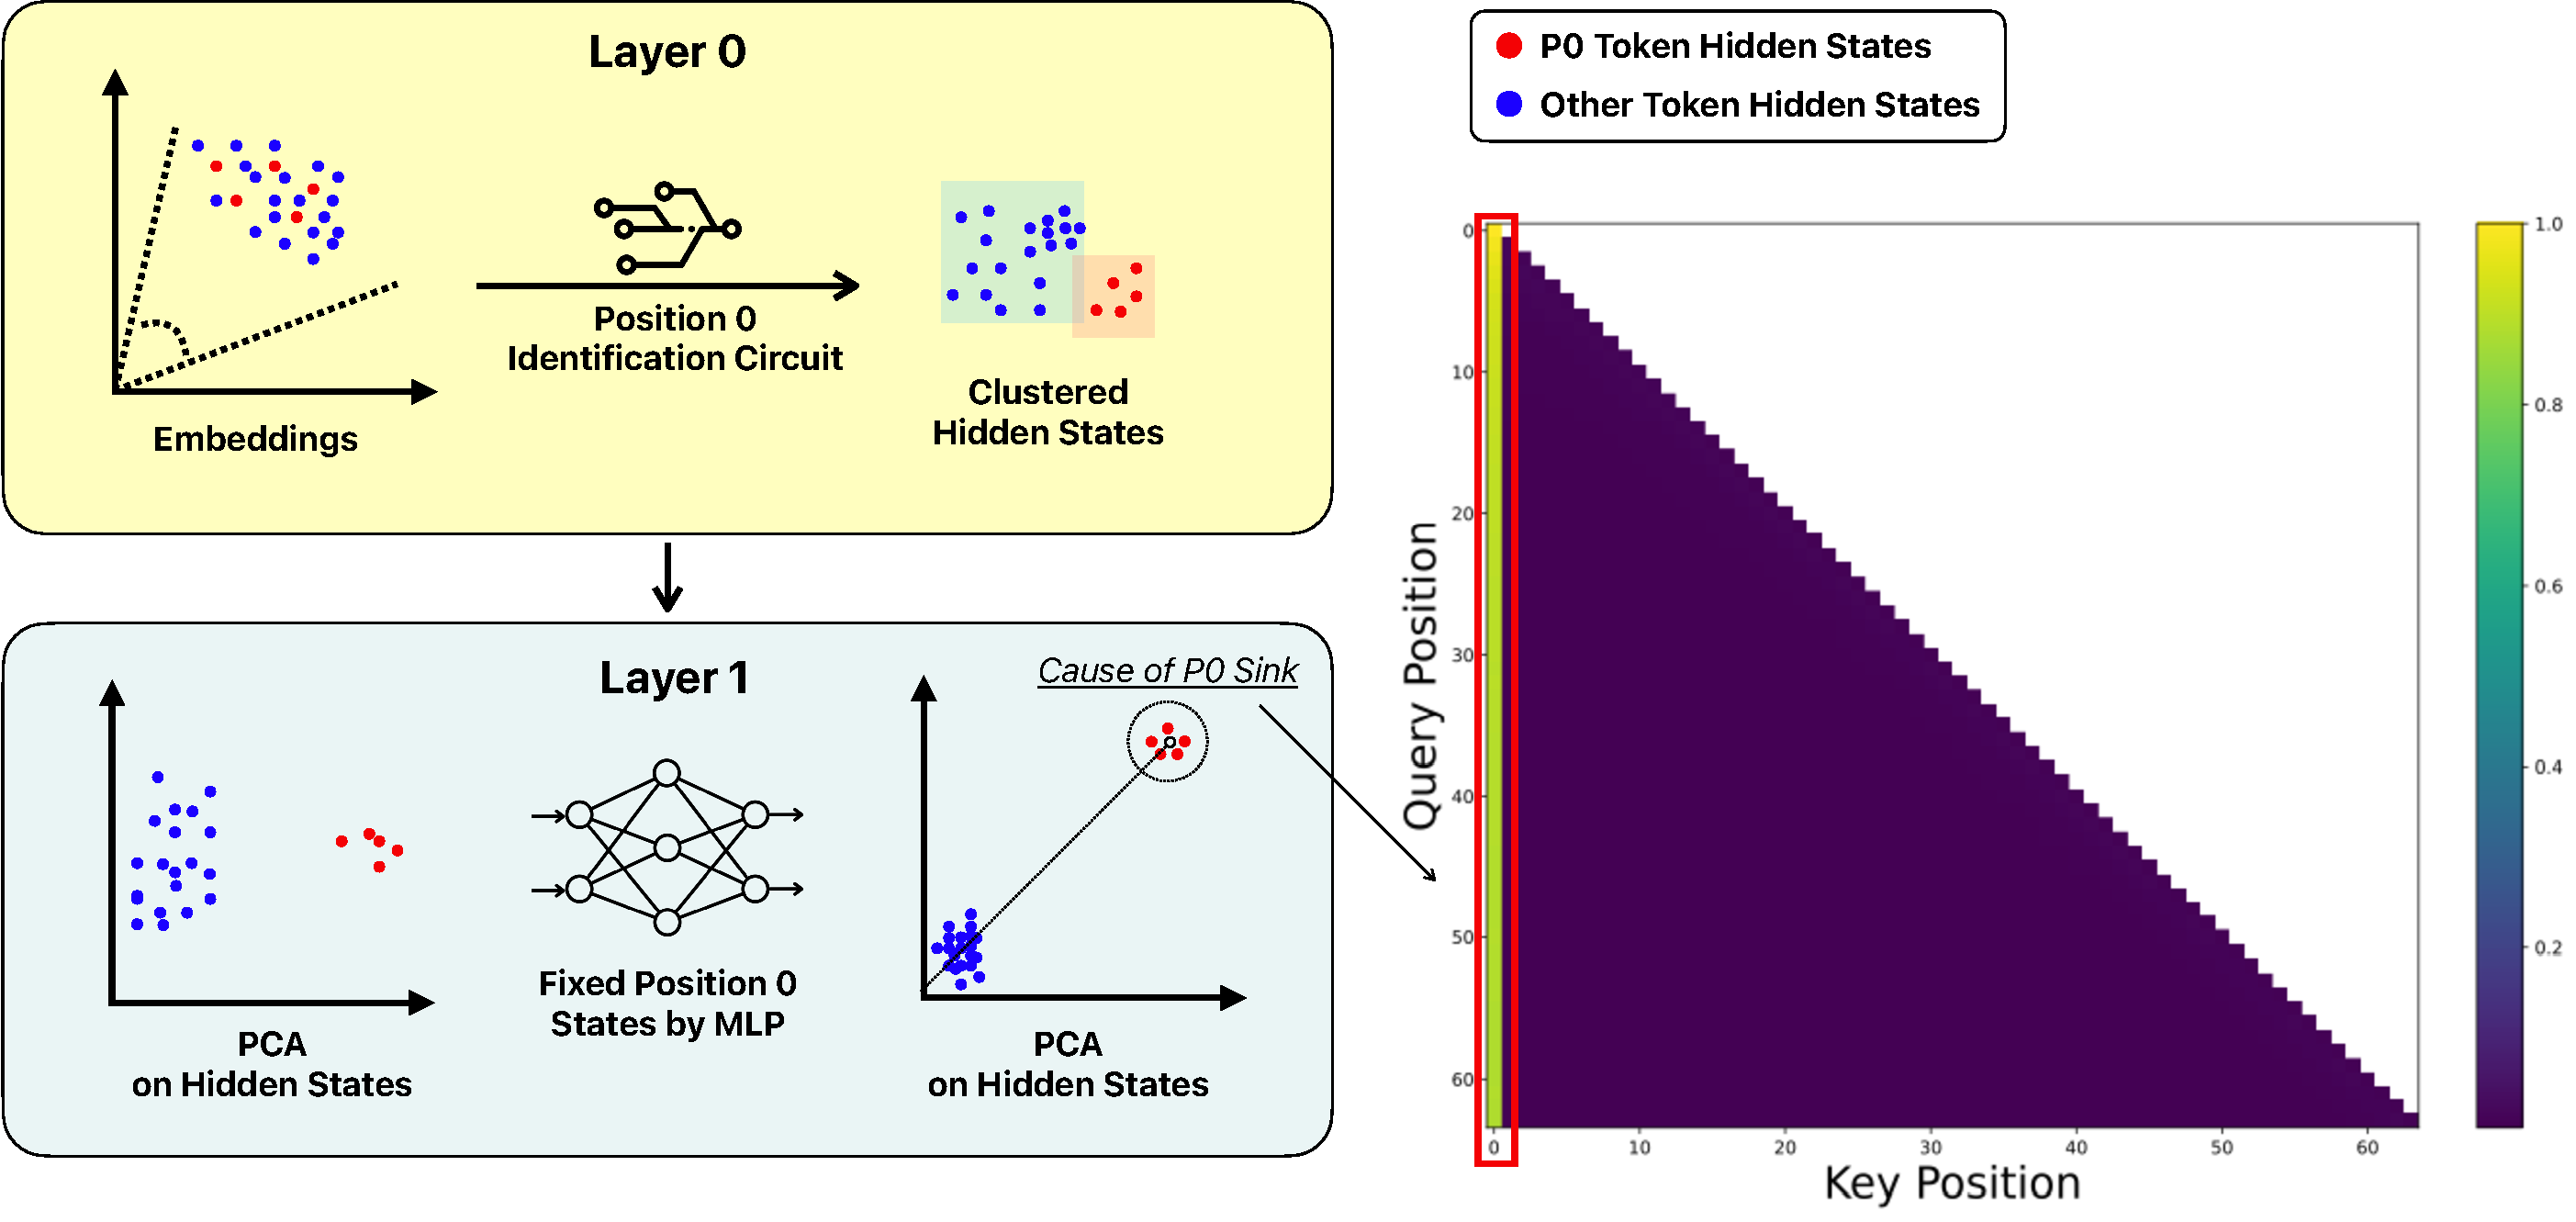
\includegraphics[width=0.95\linewidth]{figures/fig9/Fig9-cropped.pdf}
    \caption{Overview of the proposed \textbf{P0-Sink Circuit}. Within just two transformer blocks, the model learns to identify the position-zero (P0) token and amplify it into a fixed high-norm representation, which gives rise to the attention sink effect.}
    \label{fig-P0SC}
    \vspace{-1em}
\end{figure}

Auto-regressive language models tend to allocate disproportionately large attention to initial tokens. This phenomenon, the \textbf{attention sink}, reflects how softmax attention assigns probability~\citep{xiao2024efficientstreaminglanguagemodels}. Sinks also appear at non-initial positions, where excessive and persistent focus on certain tokens can interfere with effective reasoning and reduce model accuracy~\citep{yu2024unveilingharnessinghiddenattention}. Suppressing these sinks often leads to improved performance.

The main exception is the model’s consistent emphasis on the \textit{\textbf{first}} token of the input. This  \textbf{position-zero (P0) sink} is correlated with improved predictions and is used in several downstream applications \citep{xiao2024efficientstreaminglanguagemodels,han-etal-2024-lm, chen2024magicpiglshsamplingefficient}. 
Understanding why this effect emerges and how it is implemented within the model’s internal computation is a central objective of this study. 

To this end, we conduct a deep investigation of the P0 sink. Firstly, we perform an ablation study on the Beginning-Of-Sequence (\texttt{[BOS]}) token. The results show that removing \texttt{[BOS]} only affects the first-layer attention pattern in modern LLMs~\citep{grattafiori2024llama3herdmodels}, suggesting that the P0 sink is not merely a byproduct of \texttt{[BOS]} semantics, but rather a more fundamental mechanism.
To reveal this mechanism, we propose the \textbf{P0-Sink Circuit}, a simple yet effective architectural component that exploits the asymmetry of the causal attention mask. This circuit enables the model to reliably detect position zero and transform it into a deterministic representation with amplified $\ell_2$ norm. Such a high-norm, fixed-direction hidden state directly triggers the P0 sink effect, aligning with observations from previous studies~\citep{gu2025attentionsinkemergeslanguage, cancedda2024spectralfiltersdarksignals}.

To empirically validate the formation of this mechanism, we pre-train a 30B-A3B MoE model from scratch and track the evolution of its attention patterns. We find that P0 sink first emerges in deep layers, temporarily diffuses across early positions in shallow layers, and converges with a P0-Sink Circuit within the first two layers.


% While prior work has proposed hypotheses highlighting the functional importance of the P0 sink, the concrete mechanisms by which large language models implement this behavior remain unclear. 
% To bridge this gap, we conduct a series of experiments across a range of modern LLMs~\citep{yang2025qwen3technicalreport, qwen2025qwen25technicalreport, olmo2025olmo3, grattafiori2024llama3herdmodels, jiang2023mistral7b, biderman2023pythiasuiteanalyzinglarge, zhang2022optopenpretrainedtransformer}, using the FineWeb-Edu dataset~\citep{lozhkov2024fineweb-edu} as our primary corpus for analysis.

% \newpage

In this work, we make the following contributions\footnote{All experiments are conducted on a subset of FineWeb-Edu dataset~\citep{lozhkov2024fineweb-edu}}:
\begin{enumerate}
    \item We demonstrate that the position-zero sink (\textbf{P0 sink}) arises from causal-masking asymmetry rather than \texttt{[BOS]} semantics. 
    % Removing the \texttt{[BOS]} token exposes the mechanisms responsible for the position-zero sink.
    \item We formalize the \textbf{P0-Sink Circuit}, a two-layer mechanism that exploits this asymmetry to generate a fixed and high-norm representation at position zero, which provides a consistent reference point for attention heads throughout the network.
    % Layer 0 establishes the positional distinction and Layer 1 amplifies the norm of the position-zero vector. We formalize this interaction using a cone-based model of value vectors, where this circuit provides a consistent reference point for attention heads throughout the network.
    \item We characterize the formation of P0-Sink Circuit as a three-stage process during pre-training: emerging in deeper layers, spreading among early positions in shallow layers, and concentrating in the first two layers.
    % Our findings can help monitor pretraining progress, assess data quality, and inform decisions on whether further training is needed.
\end{enumerate}

\begin{figure}[t]
    \centering
    \begin{minipage}[b]{0.95\linewidth} 
        \centering
        \begin{subfigure}[b]{0.95\linewidth} 
            \centering
            \caption{Qwen3-4B, $\ell_2$ Norm of Hidden States}
            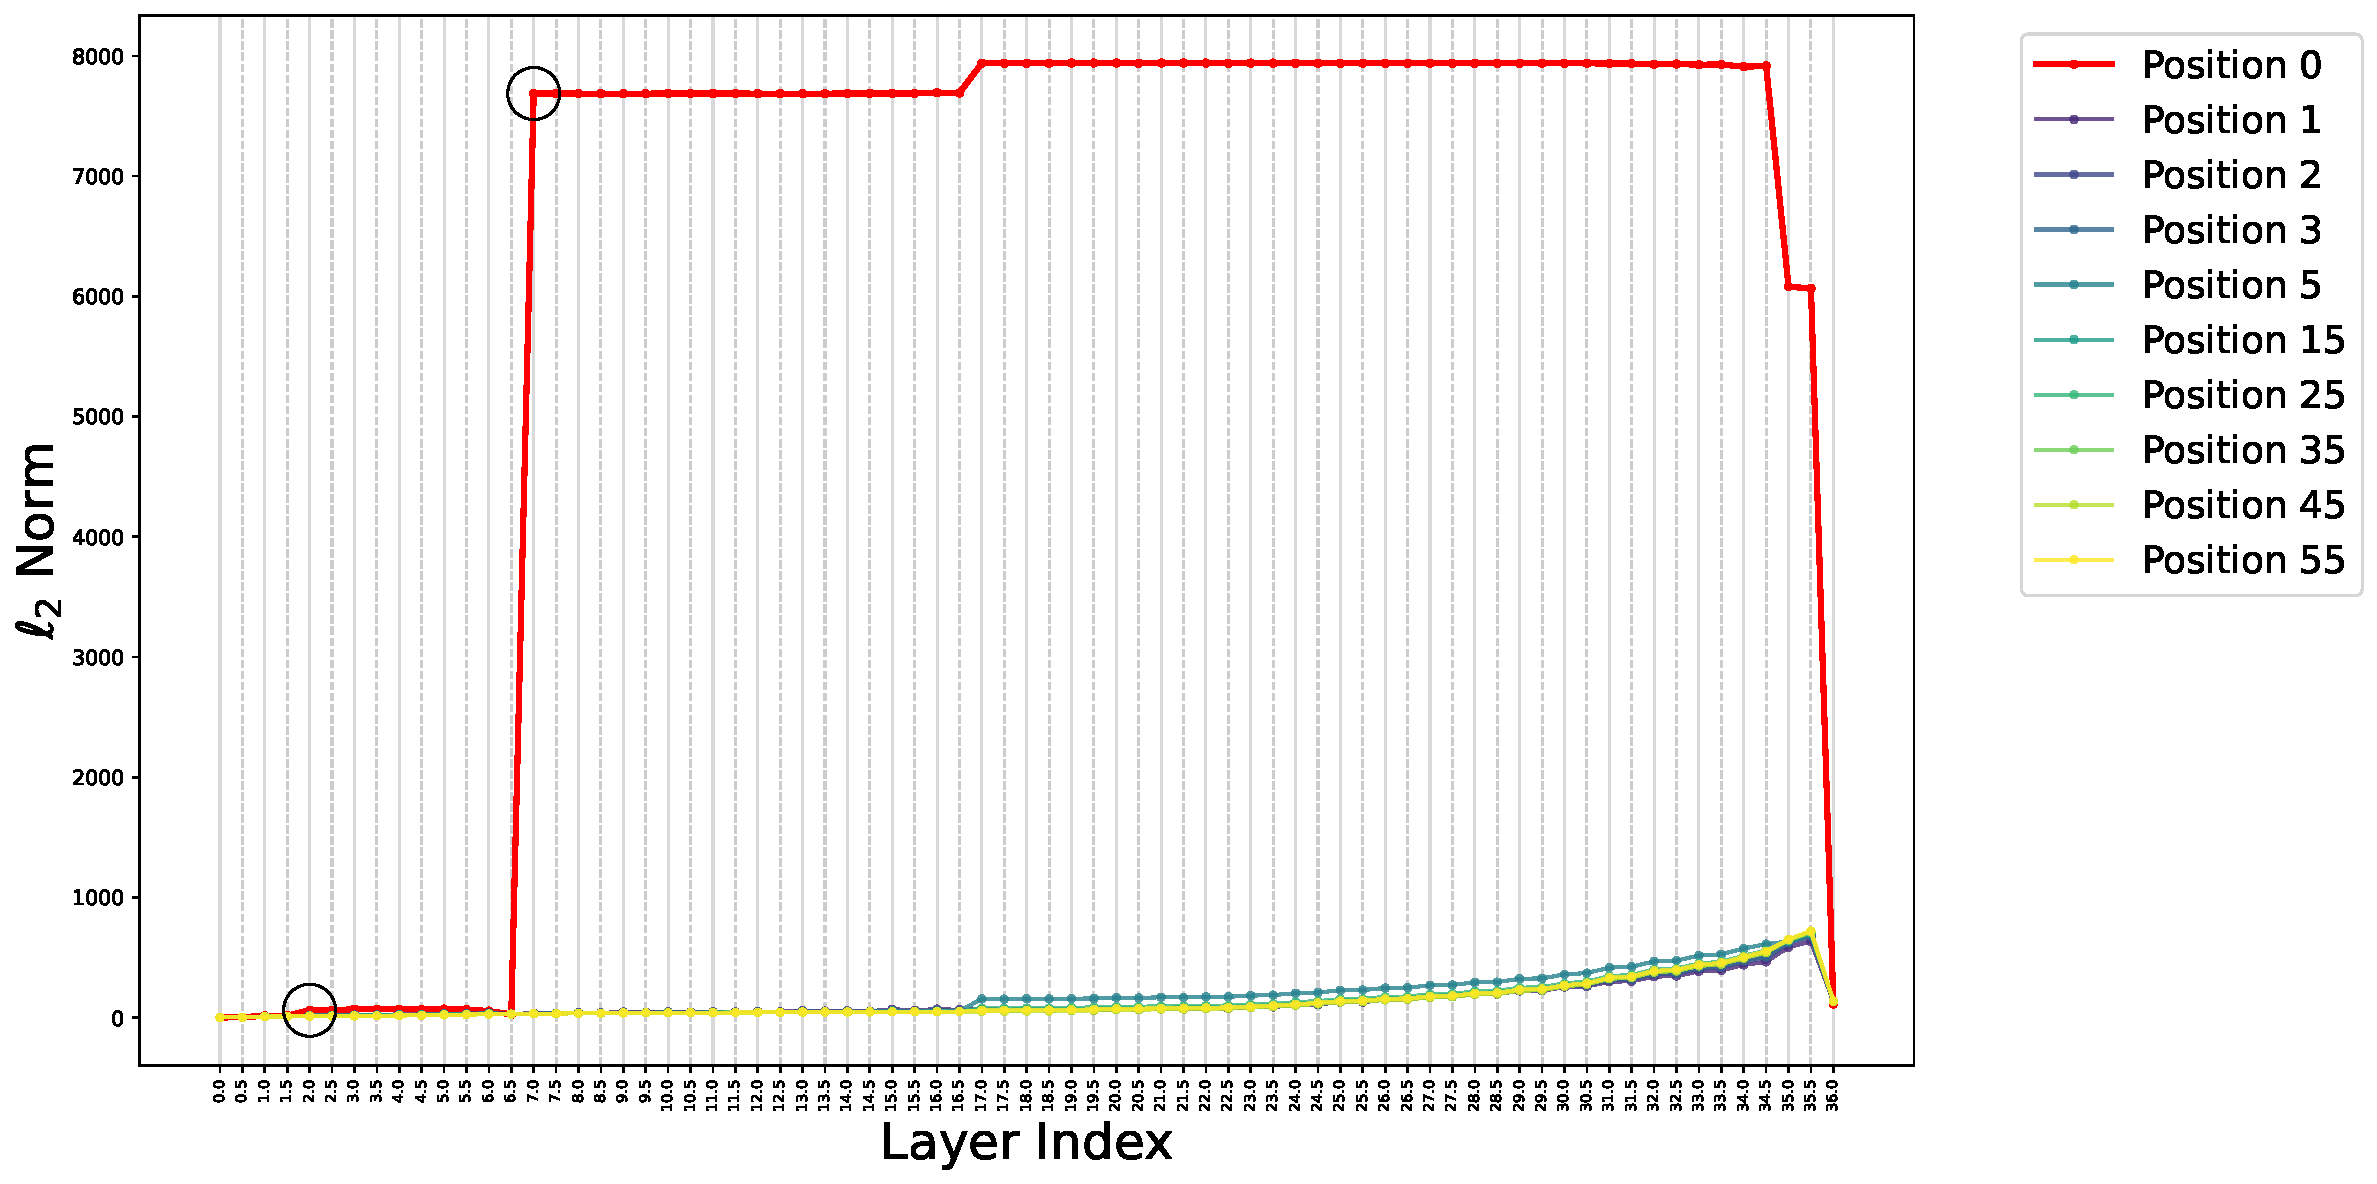
\includegraphics[width=0.95\linewidth]{figures/fig1/fig1_2_qwen.pdf}
        \end{subfigure}
    \end{minipage}
    \begin{minipage}[b]{0.94\linewidth} 
        \begin{subfigure}[b]{0.47\linewidth} 
            \centering
            \caption{Layer 2 Average Attention Score}
            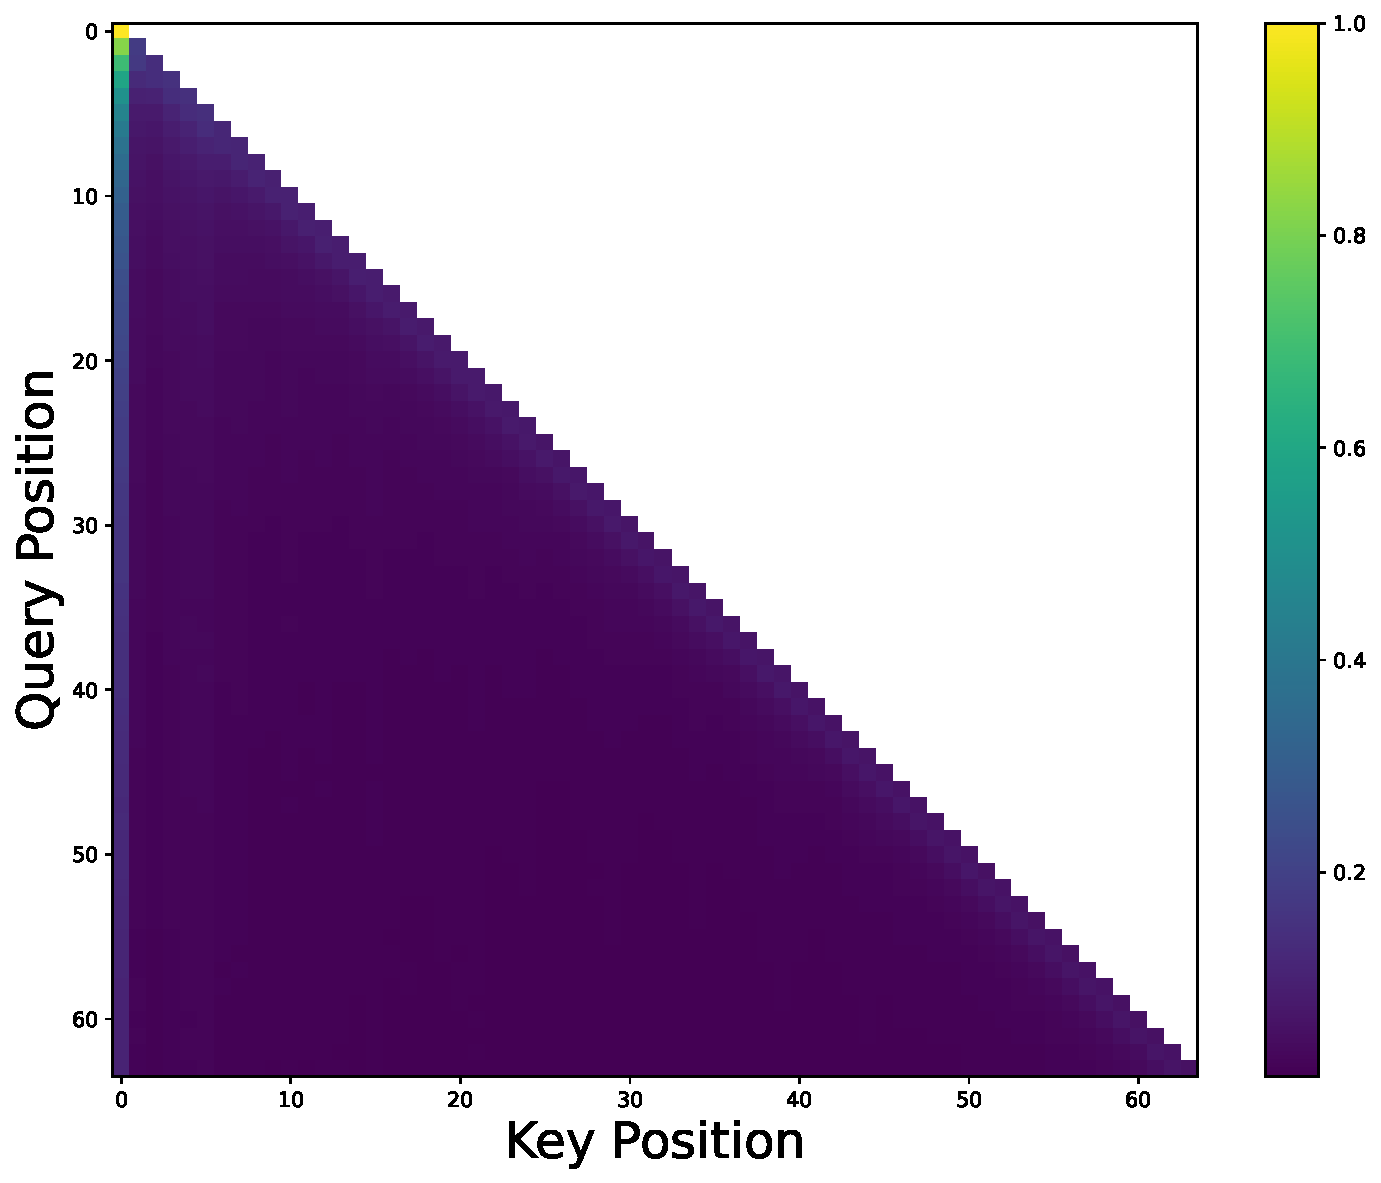
\includegraphics[width=\linewidth]{figures/fig1/fig1_1_qwen_layer2.pdf}
        \end{subfigure}
        \begin{subfigure}[b]{0.47\linewidth}
            \centering
            \caption{Layer 7 Average Attention Score} 
            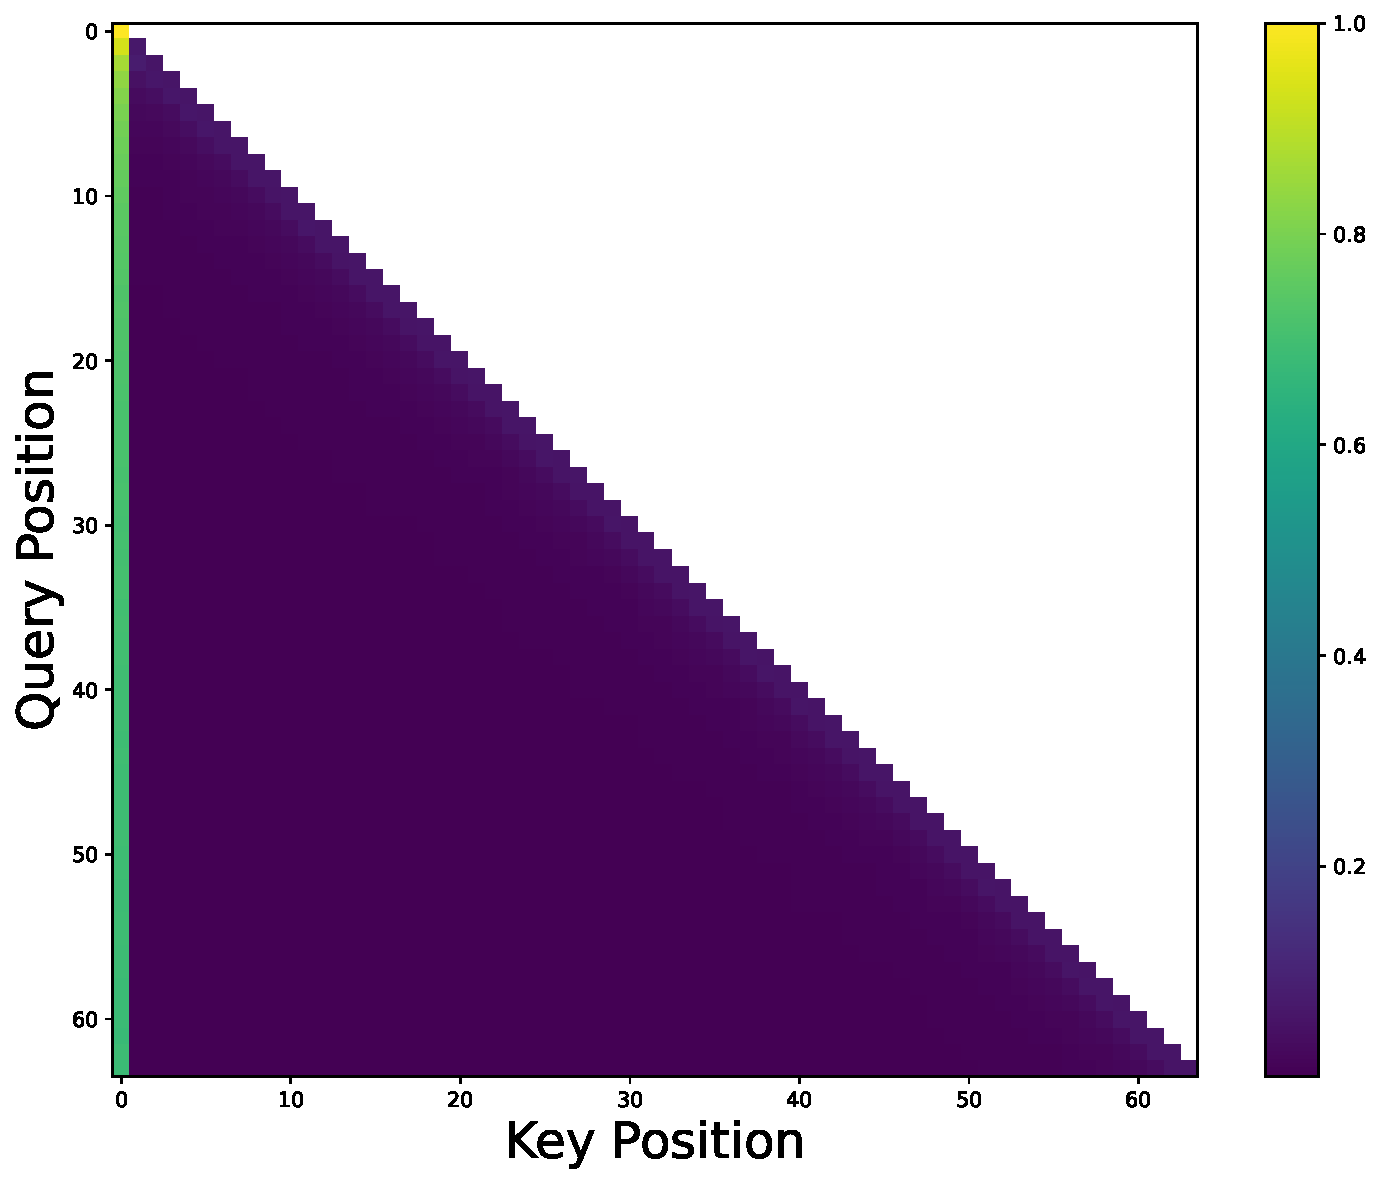
\includegraphics[width=\linewidth]{figures/fig1/fig1_1_qwen_layer7.pdf}
        \end{subfigure}
        \vspace{-0.5em}
        \caption{Layer-wise $\ell_2$ norm of hidden states and attention score heat maps in Qwen3-4B. Although this model has no \texttt{[BOS]} token, its position-zero (P0) sink appears after layer 2 and becomes pronounced after layer 7, alongside an increase in the $\ell_2$ norm at position zero. Half-integer layer indices denote attention outputs after the residual connection.}
        \label{fig-qwen-l2-and-attn-sink}
    \end{minipage}
    \vspace{-1em}
\end{figure}

\section{Related Works}

\begin{table}[t]
\resizebox{\linewidth}{!}{
\begin{tabular}{l|l|cccccccc}
\toprule
\multicolumn{2}{l|}{\textbf{First Token Repeat Time (n)}}        & n=1           & n=2           & n=3           & n=4           & n=5           & n=6           & n=7           & n=8           \\
\midrule
\multirow{2}{*}{\textbf{Llama-3.2-1B}} & w/ \texttt{[BOS]}  & \textbf{3.22} & \textbf{3.27} & \textbf{3.36} & \textbf{3.46} & 3.56          & 3.68          & 3.80          & 3.92          \\
                                                & w/o \texttt{[BOS]} & 3.32          & 3.36          & 3.42          & 3.48          & \textbf{3.53} & \textbf{3.58} & \textbf{3.62}          & \textbf{3.66}          \\
\midrule
\multirow{2}{*}{\textbf{Llama-3.2-3B}} & w/ \texttt{[BOS]}  & \textbf{2.97} & \textbf{3.01} & \textbf{3.07} & \textbf{3.15} & 3.23          & 3.33          & 3.43          & 3.53          \\
                                                & w/o \texttt{[BOS]} & 3.06          & 3.10          & 3.15          & 3.19          & \textbf{3.22} & \textbf{3.26} & \textbf{3.29} & \textbf{3.32} \\
\midrule
\multirow{2}{*}{\textbf{Llama-3.1-8B}} & w/ \texttt{[BOS]}  & \textbf{2.66} & \textbf{2.68} & \textbf{2.72} & \textbf{2.76} & \textbf{2.80} & \textbf{2.84} & \textbf{2.89} & 2.93          \\
                                                & w/o \texttt{[BOS]} & 2.79          & 2.81          & 2.83          & 2.85          & 2.86          & 2.88          & 2.89          & \textbf{2.90} \\
\midrule
\multirow{2}{*}{\textbf{Mistral-7B-v0.3}}   & w/ \texttt{[BOS]}  & 2.44          & 2.46          & 2.49          & 2.54          & 2.60          & 2.69          & 2.79          & 2.91          \\
                                                & w/o \texttt{[BOS]} & \textbf{2.39} & \textbf{2.39} & \textbf{2.40} & \textbf{2.41} & \textbf{2.41} & \textbf{2.42} & \textbf{2.43} & \textbf{2.44} \\
\bottomrule
\end{tabular}}
\caption{Loss variation under different first-token repeat counts. \textbf{Bold} indicates the smaller loss between the two settings at each repeat count. In the w/ \texttt{[BOS]} setting, the repeated token is \texttt{[BOS]}; in the w/o \texttt{[BOS]} setting, the first content token is repeated after removing \texttt{[BOS]}. For both settings, losses on repeated tokens and the original \texttt{[BOS]} position are excluded from evaluation, ensuring a consistent number of evaluated tokens across conditions for fair comparison.}
\label{bos-vs-non-bos-tab1}
% % \vspace{-2em}
\end{table}

\textbf{P0 sink} has long been the subject of investigation. \citet{cancedda2024spectralfiltersdarksignals} associate it with significantly amplified $\ell_2$ norms in the hidden states of the \texttt{[BOS]} token. They also observe linearity in these hidden states, which makes them suitable for analysis in specific linear subspaces. \citet{barbero2025llmsattendtoken} remove \texttt{[BOS]} and report a weakened sink effect, with the Sink Rate metric proposed by \citet{gu2025attentionsinkemergeslanguage}. However, it turns out that this conclusion no longer holds for more recent LLMs, where the P0 sink is driven by structural mechanisms rather than the \texttt{[BOS]} embedding.

\citet{zhang2025attentionsinkscatchtag} summarized several functional interpretations of attention sinks. For example, \citet{gu2025attentionsinkemergeslanguage} argued that attention sinks introduce a soft inductive bias into the attention mechanism, compensating for the absence of explicit bias parameters in attention layers. 
% They further showed that injecting explicit key or value biases can mitigate this effect. 
Other studies propose that the P0 sink helps deactivate redundant attention heads 
% by concentrating attention on a single uninformative position
~\citep{guo2025activedormant, sandovalsegura2025identifyingevaluatinginactiveheads}. Additionally, P0 sink has been linked to stabilizing sequence structure, reducing over-mixing of token representations, and preventing rank collapse~\citep{barbero2025llmsattendtoken, geshkovski2024emergenceclustersselfattentiondynamics}.
While these work has proposed hypotheses highlighting the functional importance of the P0 sink, the concrete mechanisms by which large language models implement this behavior remain unclear.


\section{Is \texttt{[BOS]} Token Necessary for P0 Sink?}
\label{sec2}

\begin{figure*}[ht]
    \centering
    \begin{minipage}[b]{0.48\linewidth} 
        \centering
        \begin{subfigure}[b]{0.95\linewidth} 
            \centering
            \caption{Llama3.1-8B w/ \texttt{[BOS]}, $\ell_2$ Norm of Hidden States}
            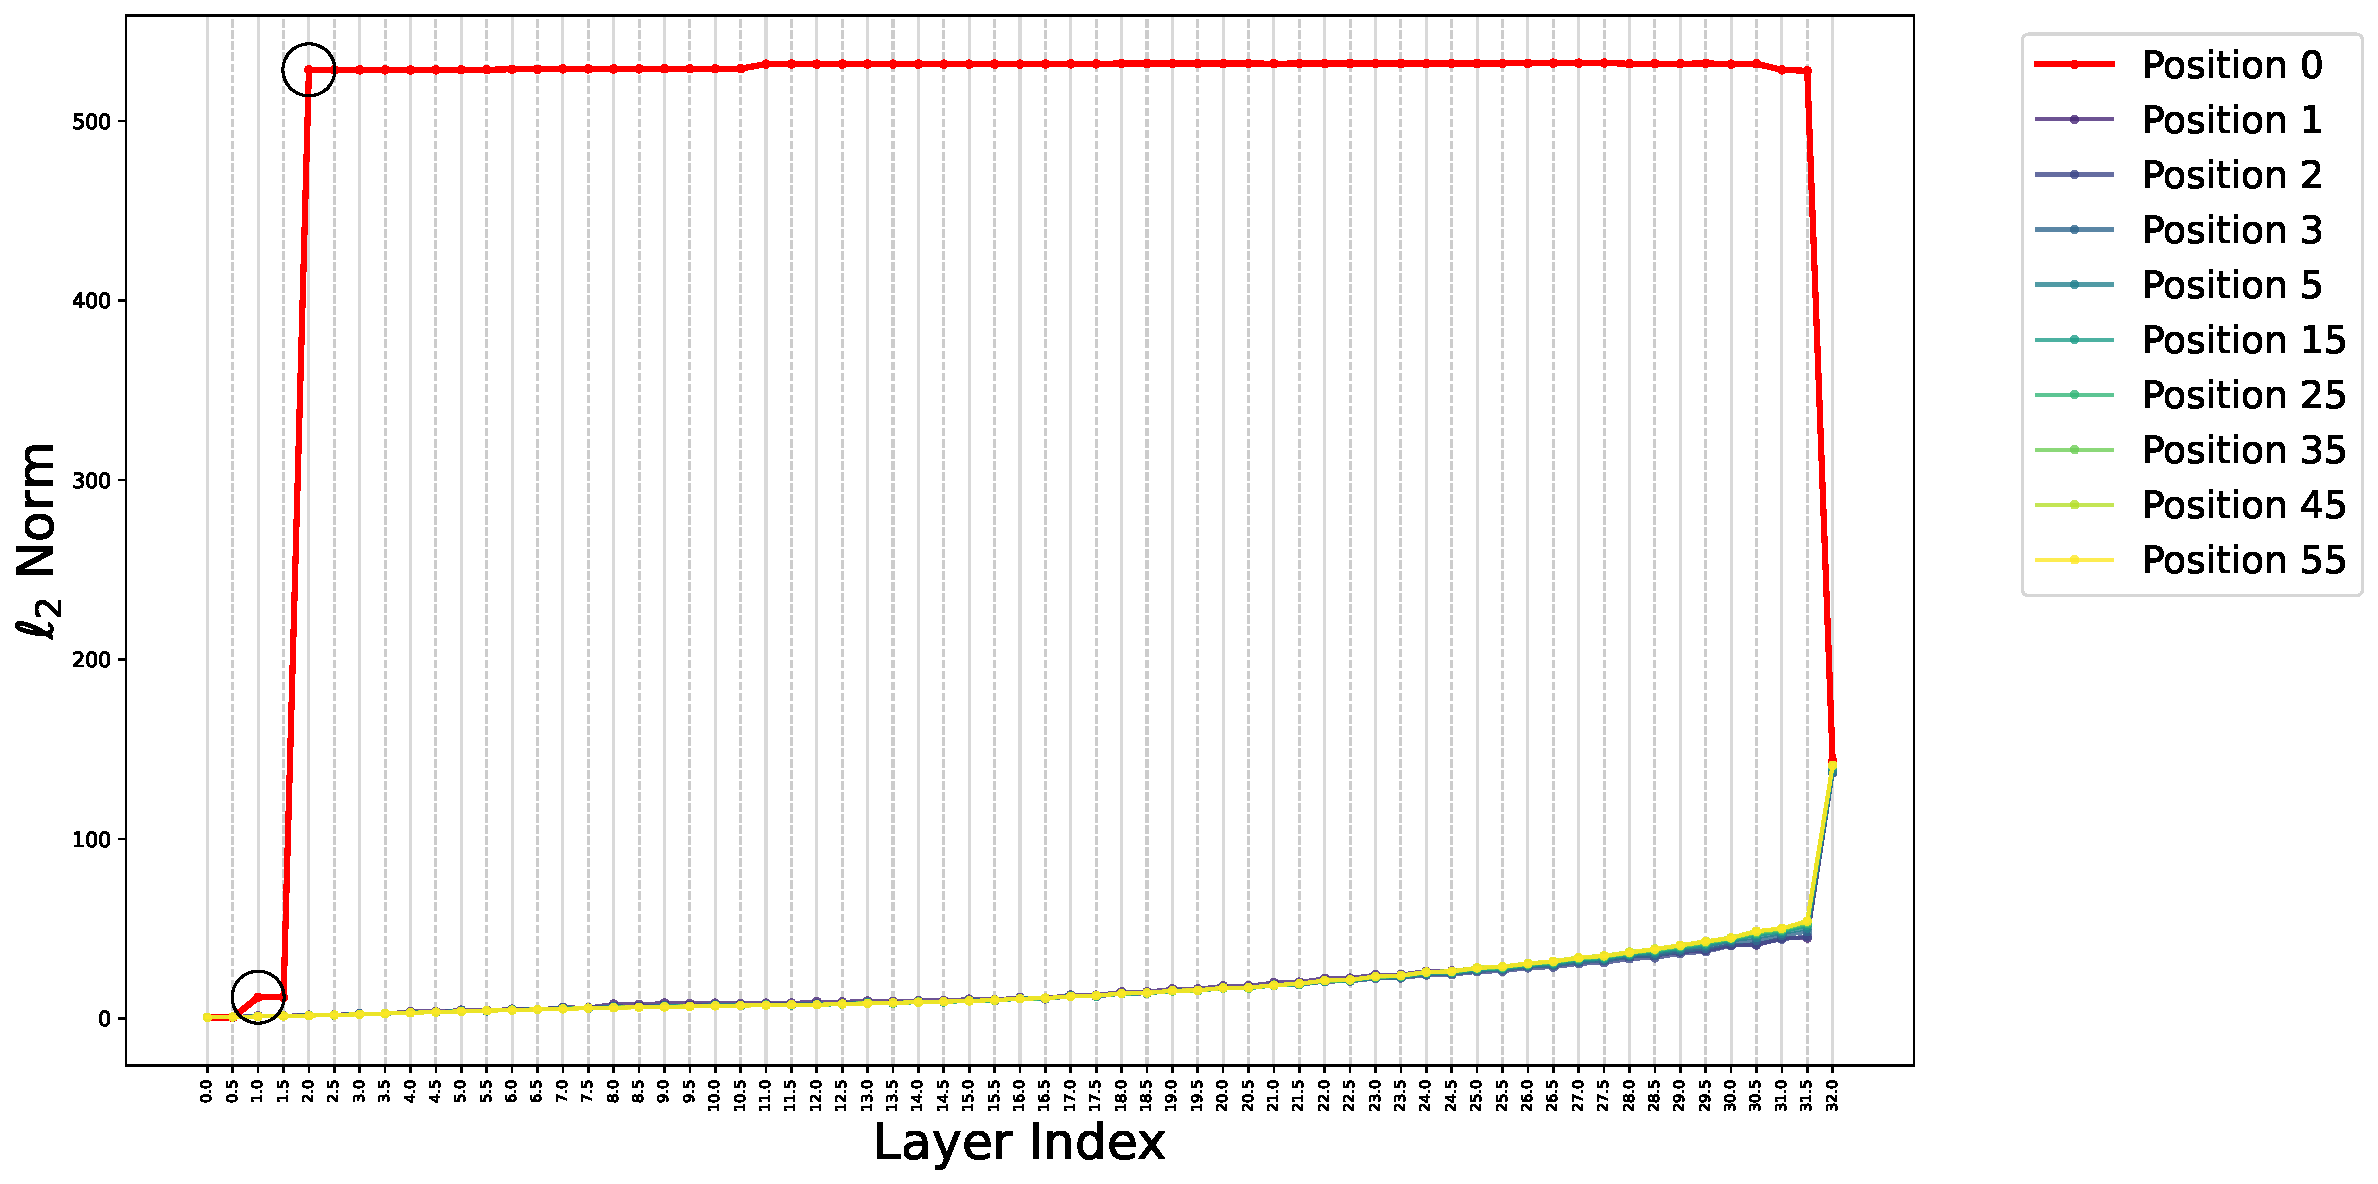
\includegraphics[width=0.95\columnwidth]{figures/fig2/fig2_2_llama_w_bos.pdf}
        \end{subfigure}
        \begin{subfigure}[b]{0.47\linewidth} 
            \centering
            \caption{\scriptsize{Layer 1 \\ Average Attention Score}}
            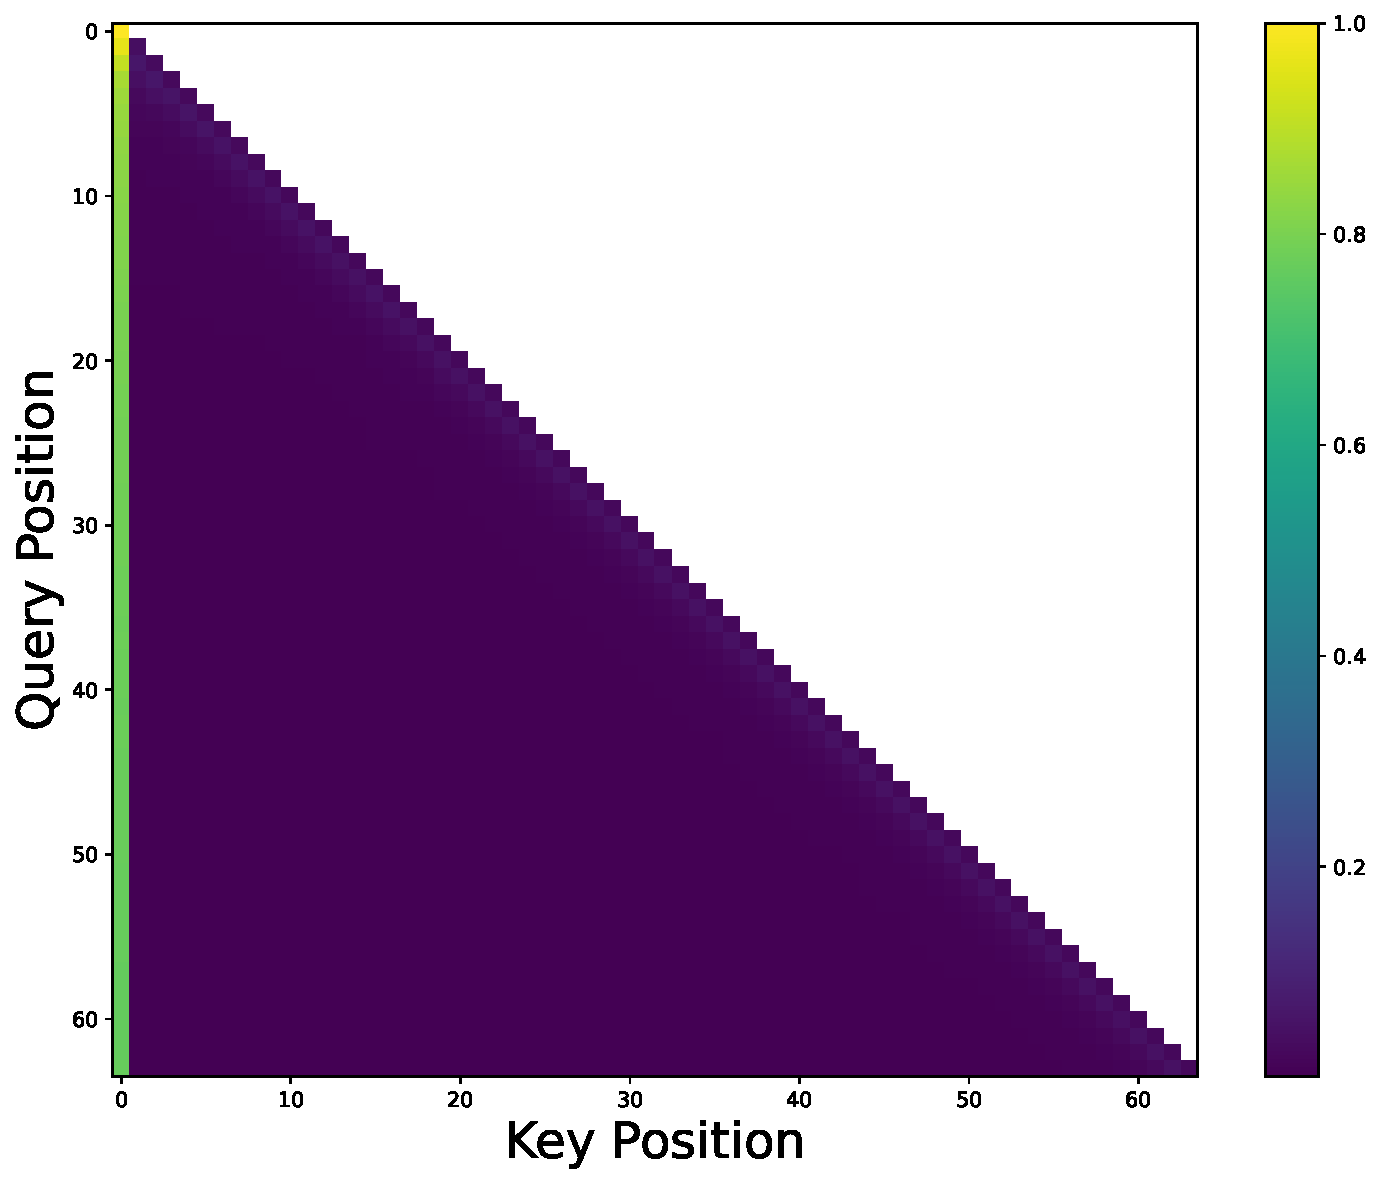
\includegraphics[width=\linewidth]{figures/fig2/fig2_1_llama_w_bos_layer1.pdf}
        \end{subfigure}
        \begin{subfigure}[b]{0.47\linewidth}
            \centering
            \caption{\scriptsize{Layer 2 \\ Average Attention Score}}
            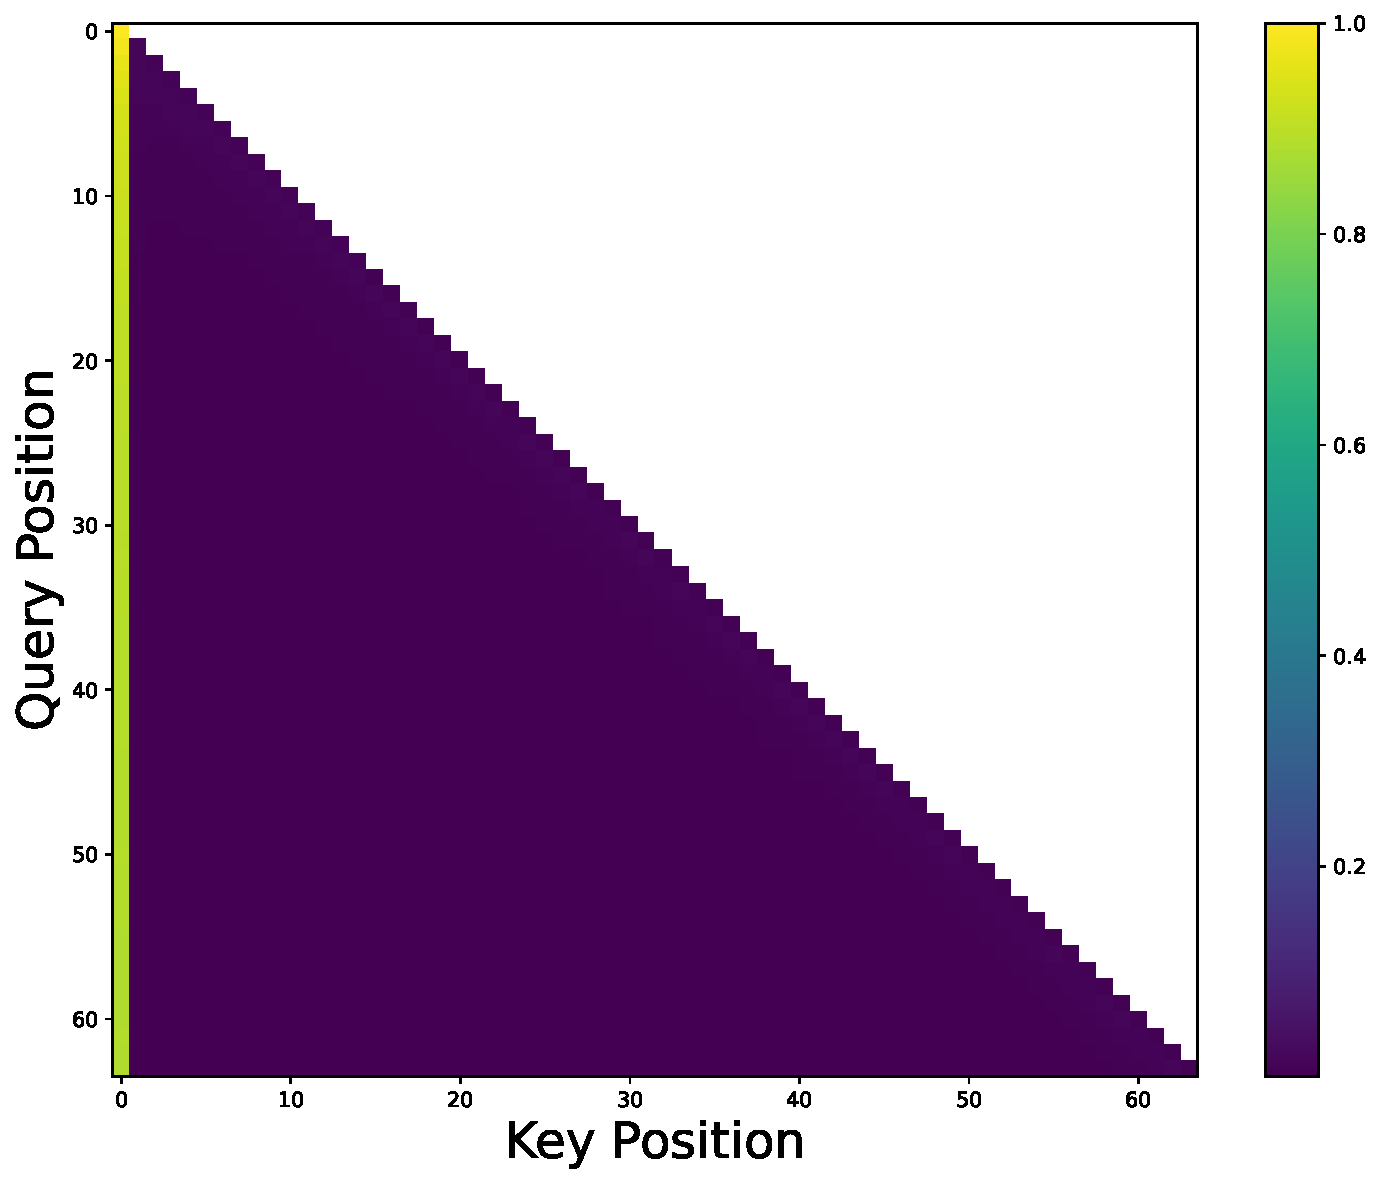
\includegraphics[width=\linewidth]{figures/fig2/fig2_1_llama_w_bos_layer2.pdf}
        \end{subfigure}
    \end{minipage}
    \begin{minipage}[b]{0.48\linewidth} 
        \centering
        \begin{subfigure}[b]{0.95\linewidth} 
            \centering
            \caption{Llama3.1-8B w/o \texttt{[BOS]}, $\ell_2$ Norm of Hidden States}
            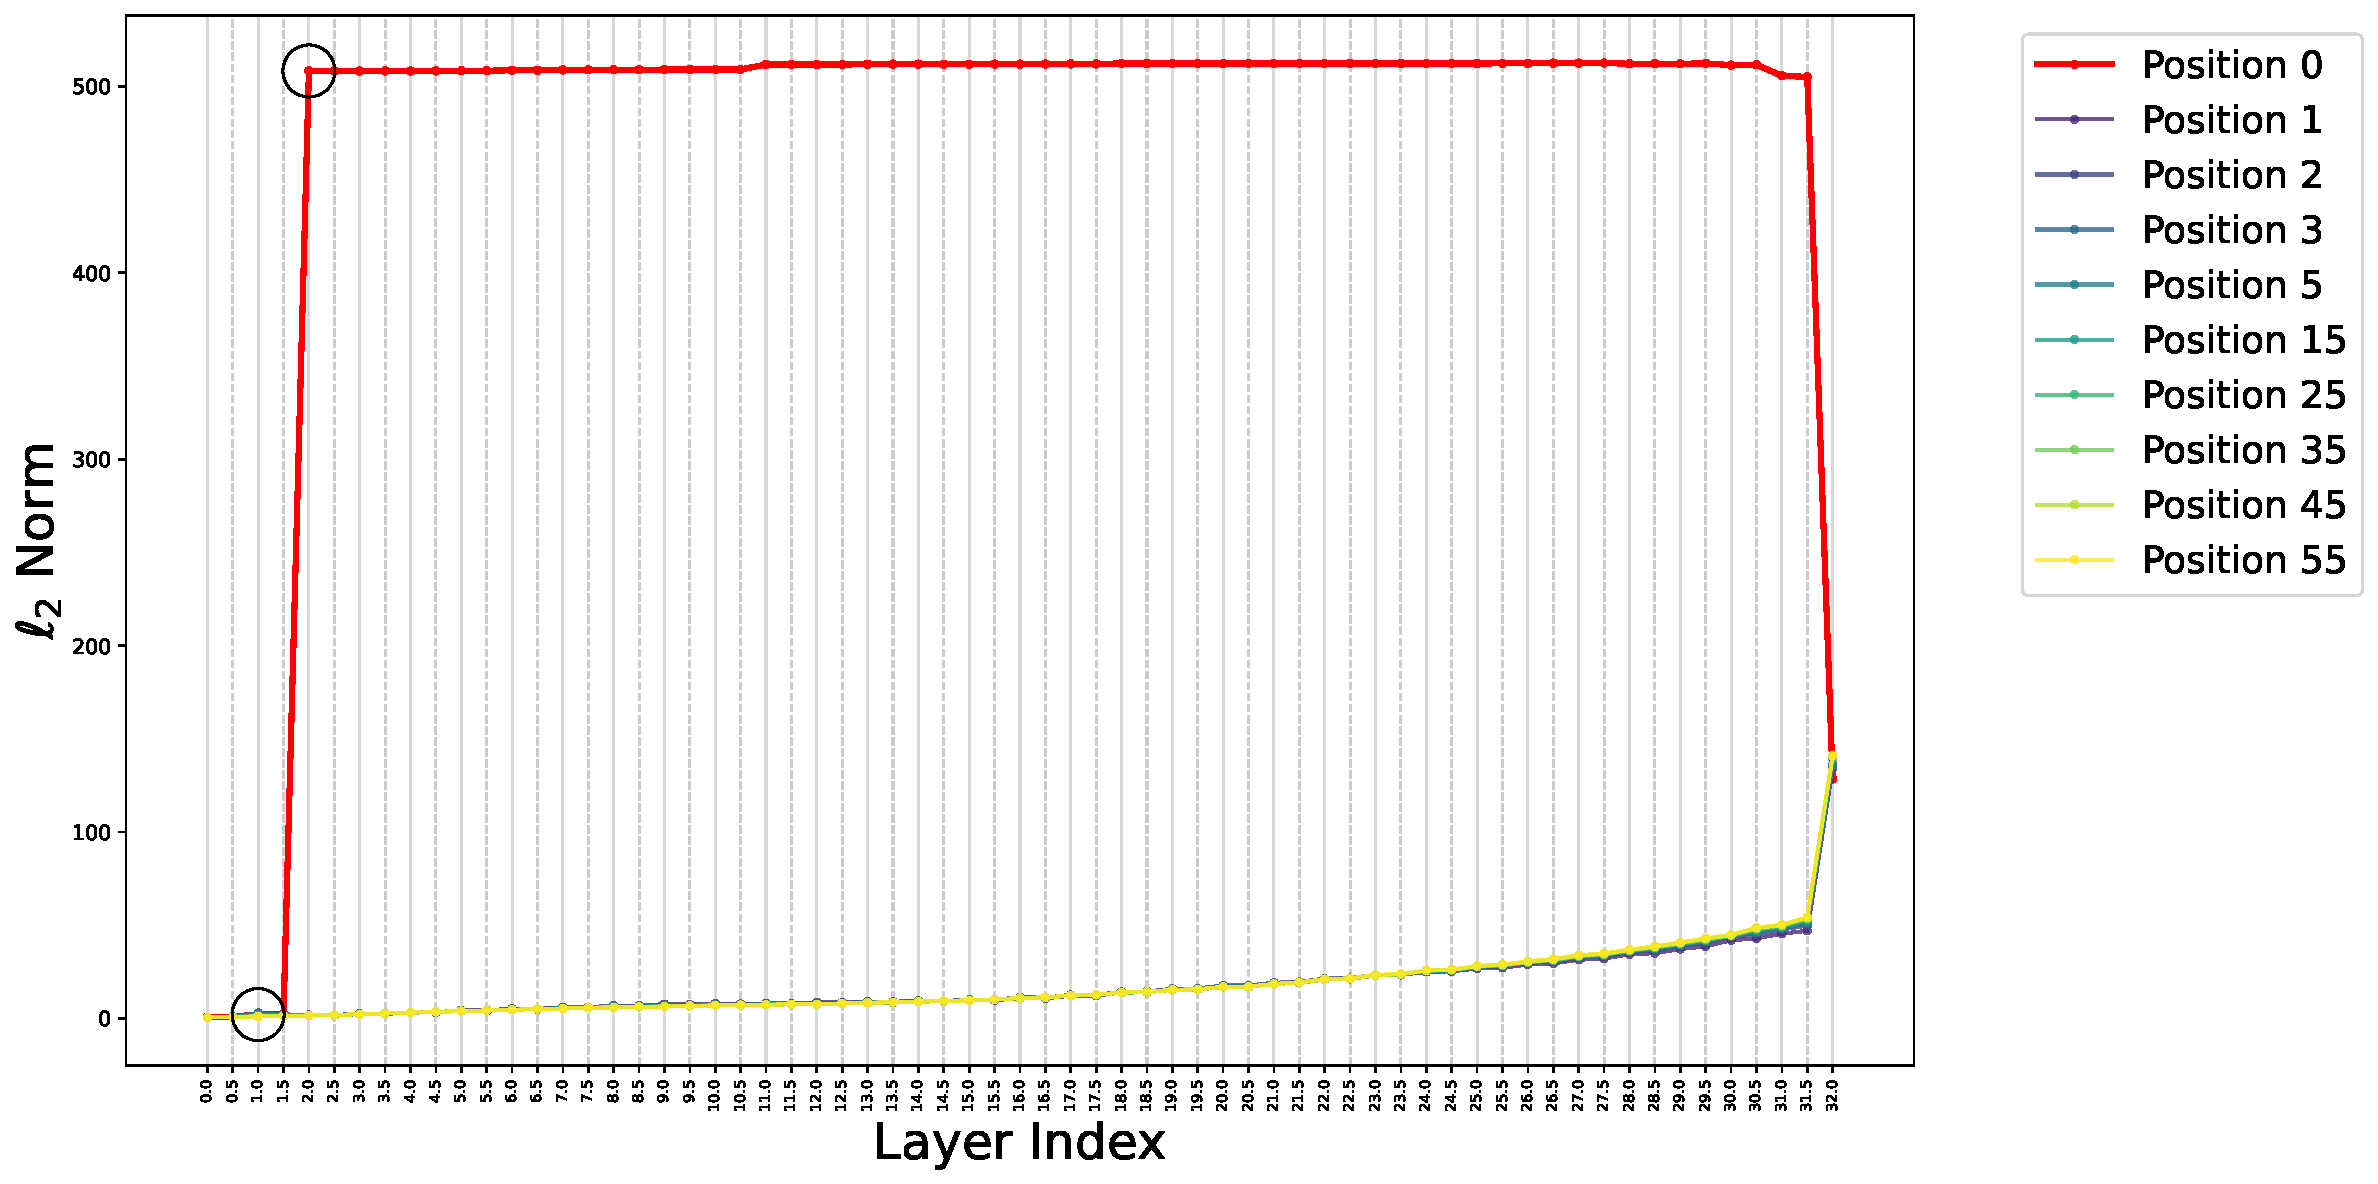
\includegraphics[width=0.95\columnwidth]{figures/fig2/fig2_2_llama_wo_bos.pdf}
        \end{subfigure}
        \begin{subfigure}[b]{0.47\linewidth} 
            \centering
            \caption{\scriptsize{Layer 1 \\ Average Attention Score}}
            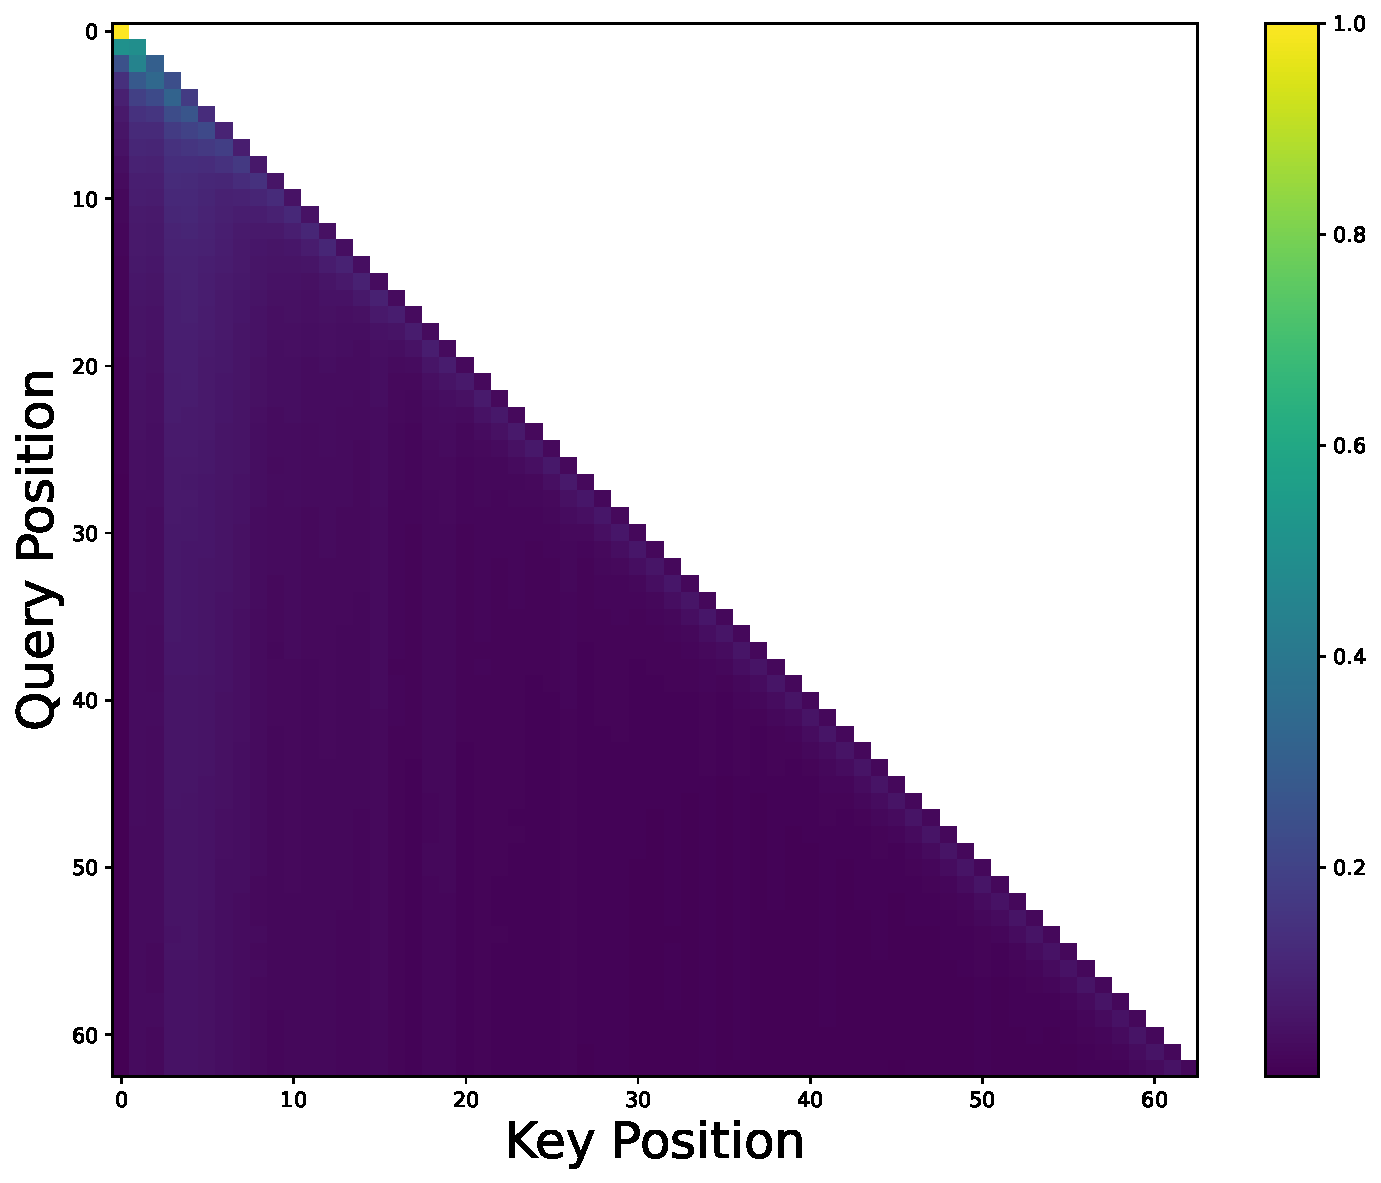
\includegraphics[width=\linewidth]{figures/fig2/fig2_1_llama_wo_bos_layer1.pdf}
        \end{subfigure}
        \begin{subfigure}[b]{0.47\linewidth}
            \centering
            \caption{\scriptsize{Layer 2 \\ Average Attention Score} }
            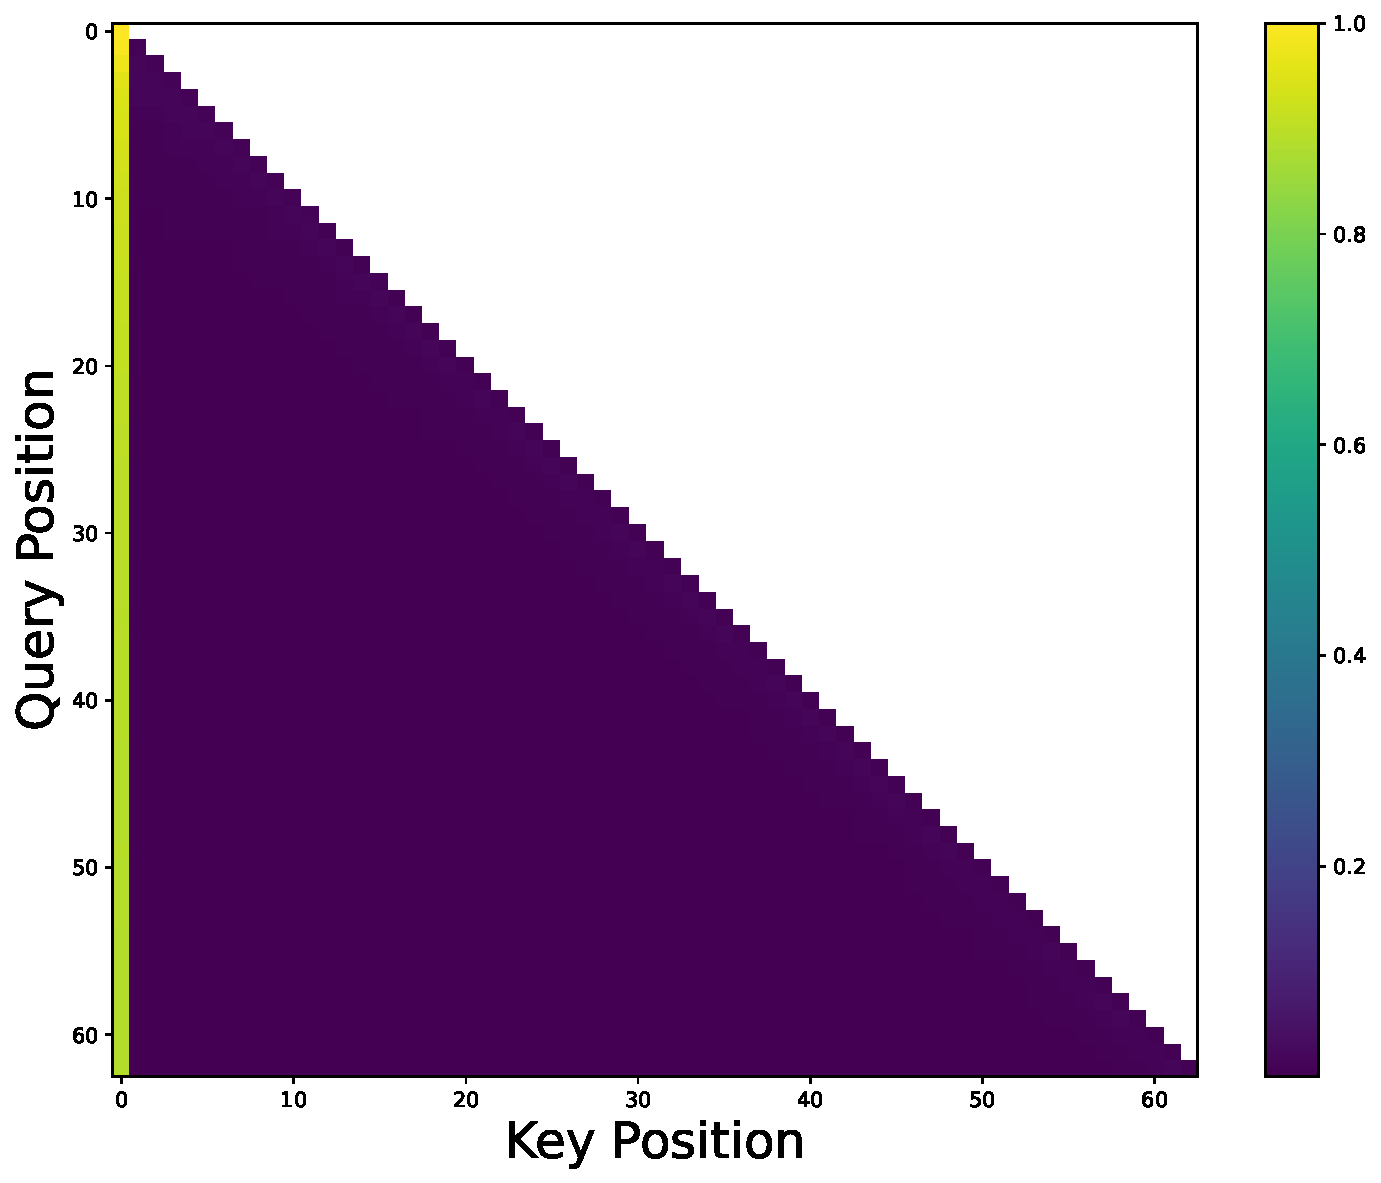
\includegraphics[width=\linewidth]{figures/fig2/fig2_1_llama_wo_bos_layer2.pdf}
        \end{subfigure}
    \end{minipage}
    \caption{Layer-wise $\ell_2$ norm of hidden states and attention score heat maps in LLaMA3.1-8B. Half-integer indices correspond to the output of attention modules after residual connection. Removing the \texttt{[BOS]} token eliminates the layer-1 attention sink and its associated $\ell_2$ norm amplification. However, due to renewed norm growth before layer 2, a position-zero (P0) sink re-emerges in the attention maps even in the absence of the \texttt{[BOS]} token.}
    \label{bos-vs-non-bos-fig1}
    % \vspace{-2em}
\end{figure*}

\begin{figure}[t]
    \centering
    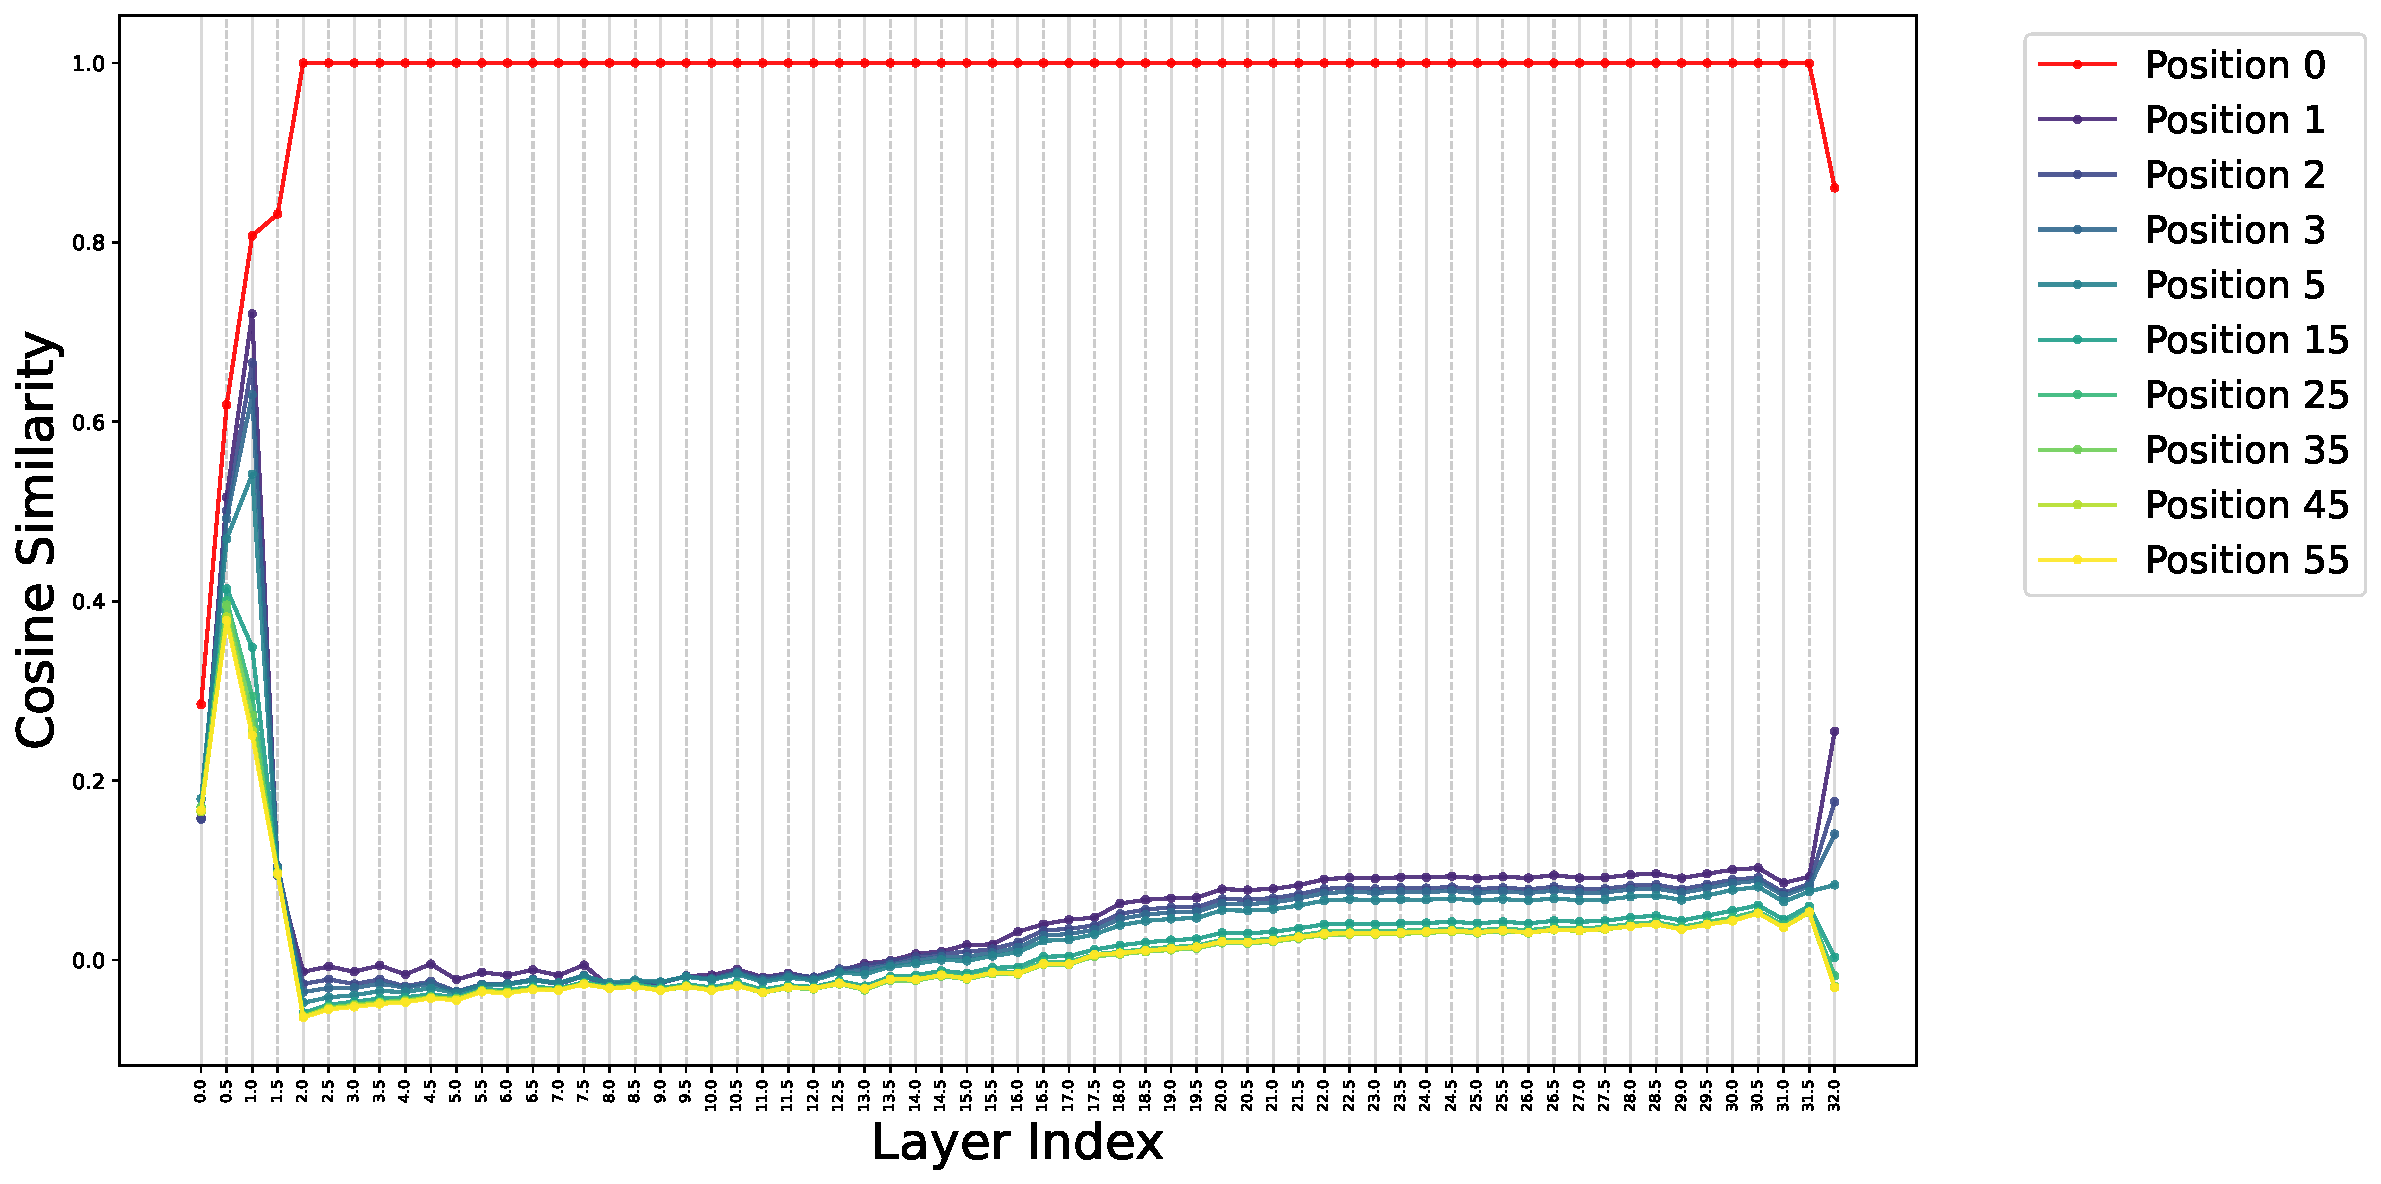
\includegraphics[width=0.95\linewidth]{figures/fig4/fig4_llama3_1_8b_cos_sim.pdf}
    \caption{Average cosine similarity among hidden states at different positions across inputs, along with the corresponding mean hidden state vectors at position zero in LLaMA3.1-8B. Half-integer indices indicate the outputs of attention modules after residual addition. The \texttt{[BOS]} token has been removed, so position zero corresponds to the first non-\texttt{[BOS]} token.}
    \label{8b_no_bos_cos_sim_fig}
    % \vspace{-2em}
\end{figure}

\citet{cancedda2024spectralfiltersdarksignals} identify a key internal mechanism underlying the attention sink phenomenon: the hidden states of a fixed \texttt{[BOS]} token exhibit significantly amplified $\ell_2$ norms after passing through certain transformer layers. 
Building on this, \citet{gu2025attentionsinkemergeslanguage} further investigate the correlation between this norm inflation and the emergence of attention sinks, showing that attention scores become disproportionately concentrated on the P0 tokens as a result.

Subsequent works have shown that the attention sink phenomenon also arises in models without an explicit \texttt{[BOS]} token \citep{sandovalsegura2025identifyingevaluatinginactiveheads}. For example, in the Qwen and OLMo model families \citep{yang2025qwen3technicalreport, qwen2025qwen25technicalreport, olmo20252olmo2furious}, the P0 token, typically corresponding to the first non-padding token, continues to attract a dominant share of attention across layers and heads. Notably, this behavior is again accompanied by a significant increase in the $\ell_2$ norm of the P0 token’s hidden states as it propagates through the network, shown in Figure \ref{fig-qwen-l2-and-attn-sink}.


In models such as LLaMA~\citep{grattafiori2024llama3herdmodels}, removing the \texttt{[BOS]} token leads to a measurable increase in training loss and degrades downstream performance~\citep{barbero2025llmsattendtoken}, suggesting that [BOS] plays a nontrivial functional role. However, as shown in Figure~\ref{bos-vs-non-bos-fig1}, a clear attention sink at position zero re-emerges after several layers even in the absence of \texttt{[BOS]}, indicating that this behavior cannot be fully explained by the \texttt{[BOS]} embedding itself. The model learns a second mechanism, operating through deeper MLP sublayers, that stabilizes the P0 representation independently of \texttt{[BOS]}.

This division of labor becomes more evident when comparing shallow versus deep layers. While \texttt{[BOS]} influences early hidden states, deeper layers consistently reconstruct a fixed direction for position zero through specific MLP sublayers, regardless of the initial token. Table~\ref{bos-vs-non-bos-tab1} further supports this view by showing that such deeper mechanisms remain robust across input perturbations.

One such perturbation arises from a known property of modern positional encoding schemes. Since position is encoded via relative or rotary mechanisms, repeating the first token causes multiple positions to share nearly identical hidden states~\citep{gu2025attentionsinkemergeslanguage}, creating a synthetic prefix pattern that deviates from the model’s training distribution—a form of out-of-distribution (OOD) shift. 
% Long-context scenarios present a complementary form of OOD stress, where the influence of the first token is diluted as the attention window spans more tokens. Despite pulling attention dynamics in opposite directions, both cases challenge the model’s ability to maintain stable structural priors.

The position-zero sink re-emerges under such diverse conditions highlights the stability of this \texttt{[BOS]}-independent mechanism.  This motivates a detailed examination of its formation, as it may offer a more general and robust inductive bias than token-based schemes, and may help LLMs maintain coherence under OOD inputs such as long contexts.

% In contrast, long-context scenarios induce a different type of OOD behavior: as the attention window expands, the influence of position zero becomes diluted across a larger number of competing tokens. Although these two forms of OOD perturbation exert opposite effects on attention allocation—one amplifying and the other diminishing the prominence of position zero—they both challenge the model’s ability to maintain consistent and robust behavior under distributional shifts.

% This contrast underscores the importance of understanding the BOS-independent mechanism behind attention sink formation. Because it continues to operate reliably under both amplification and dilution pressures, this mechanism likely reflects a more fundamental inductive bias of the architecture, rather than an artifact of special token embeddings. Its stability across diverse OOD conditions makes it not only an intriguing subject of study, but also a potentially useful handle for improving robustness in downstream applications.
% As shown in Table~\ref{bos-vs-non-bos-tab1}, the BOS-independent mechanism exhibits greater robustness in such cases. 
% The distinct behavior of Mistral \citep{jiang2023mistral7b}, which deviates from this pattern, will be discussed in a later section.



% \begin{figure*}[t]

% \begin{minipage}[b]{\linewidth} 
%     \begin{subfigure}[b]{0.75\linewidth} 
%         \centering
%         \caption{\scriptsize{Llama3.1-8B w/ [BOS], $\ell_2$ Norm of Hidden States}}
%         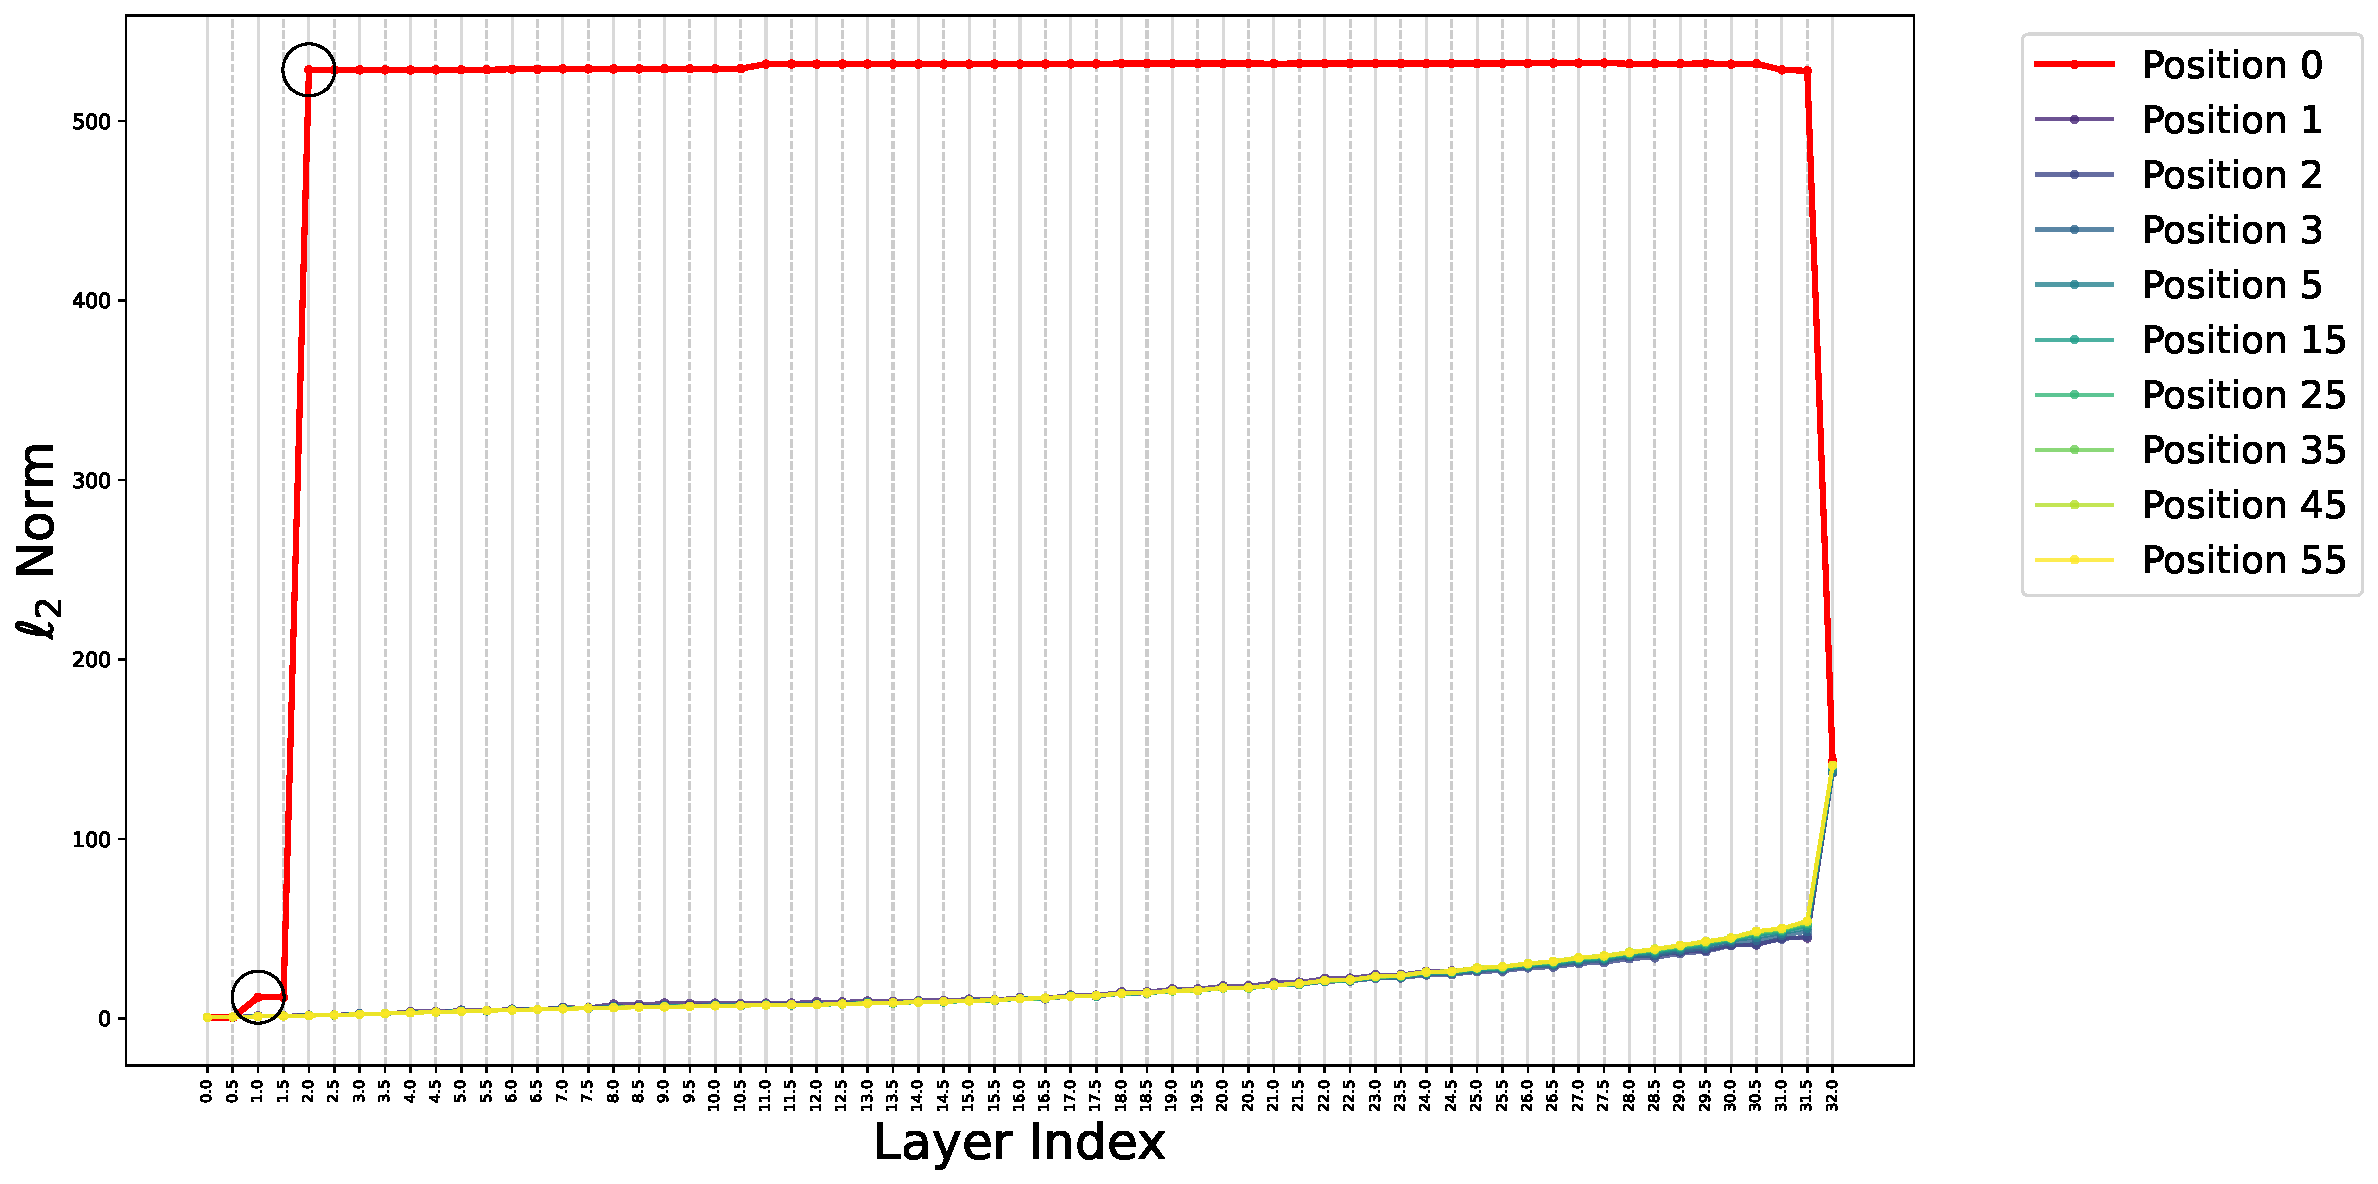
\includegraphics[width=0.95\columnwidth]{figures/fig2/fig2_2_llama_w_bos.pdf}
%     \end{subfigure}
%     \begin{subfigure}[b]{0.18\linewidth} 
%         \centering
%         \begin{subfigure}[b]{\linewidth} 
%             \centering
%             \caption{\scriptsize{Layer 1 Average Attention Score}}
%             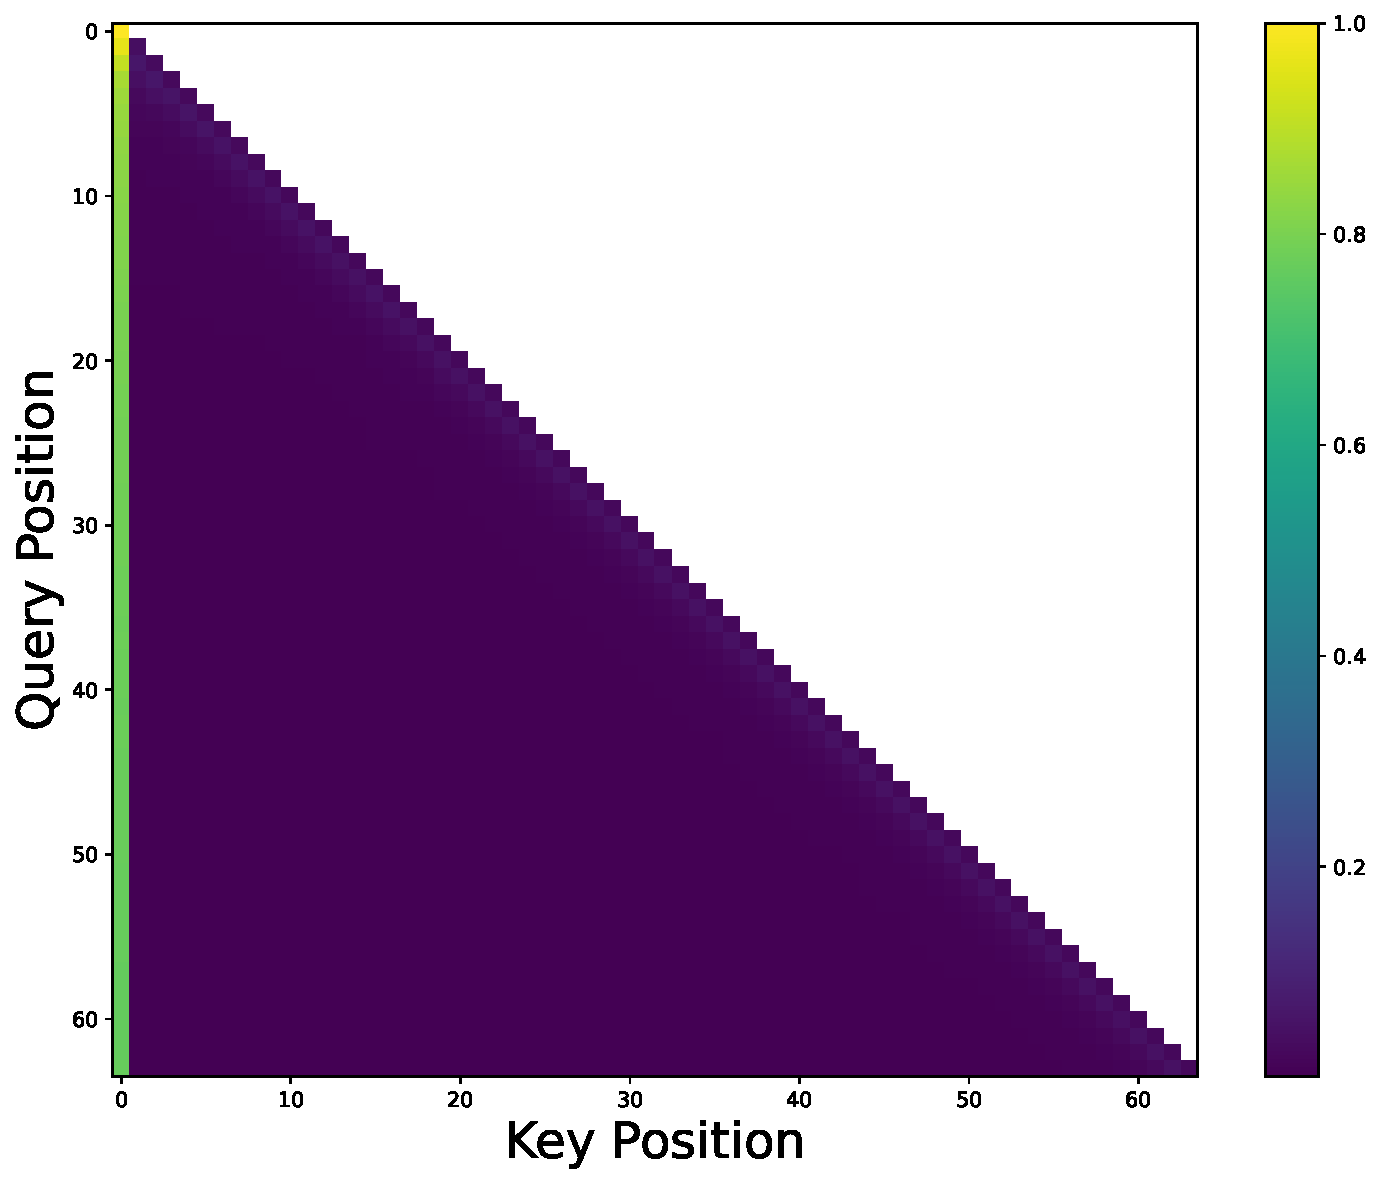
\includegraphics[width=\linewidth]{figures/fig2/fig2_1_llama_w_bos_layer1.pdf}
%         \end{subfigure}
%         \begin{subfigure}[b]{\linewidth}
%             \centering
%             \caption{\scriptsize{Layer 2 Average Attention Score}} 
%             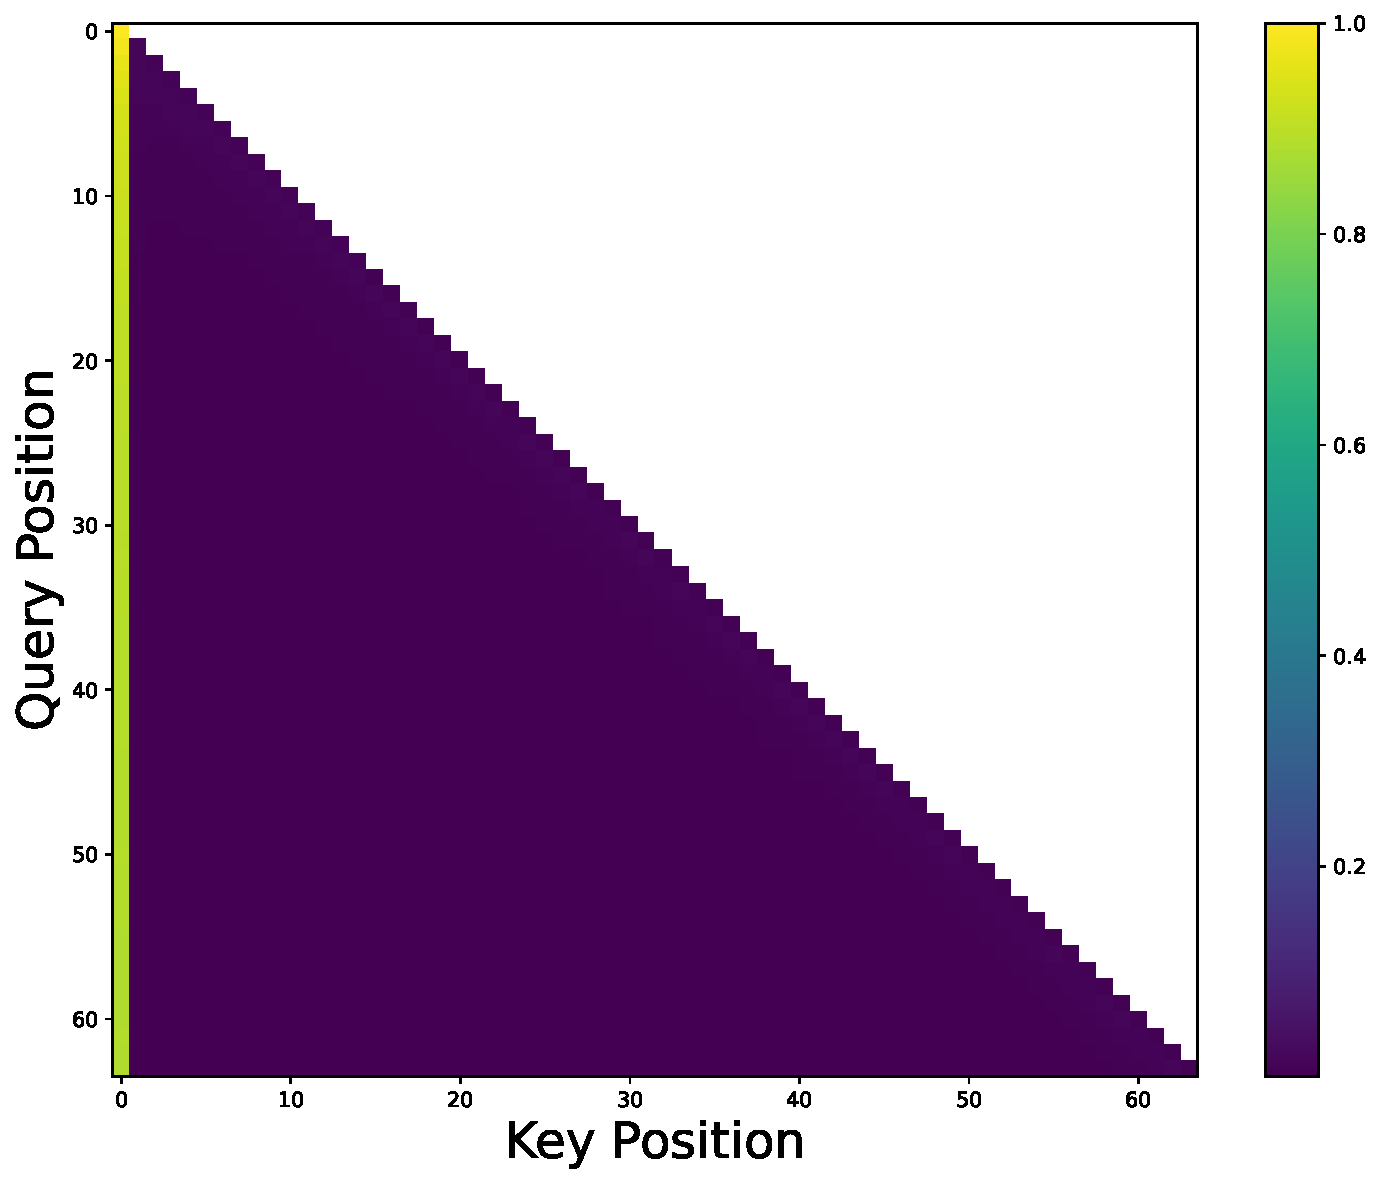
\includegraphics[width=\linewidth]{figures/fig2/fig2_1_llama_w_bos_layer2.pdf}
%         \end{subfigure}
%     \end{subfigure}
% \end{minipage}

% \begin{minipage}[b]{\linewidth} 
%     \begin{subfigure}[b]{0.75\linewidth} 
%         \centering
%         \caption{\scriptsize{Llama3.1-8B w/o [BOS], $\ell_2$ Norm of Hidden States}}
%         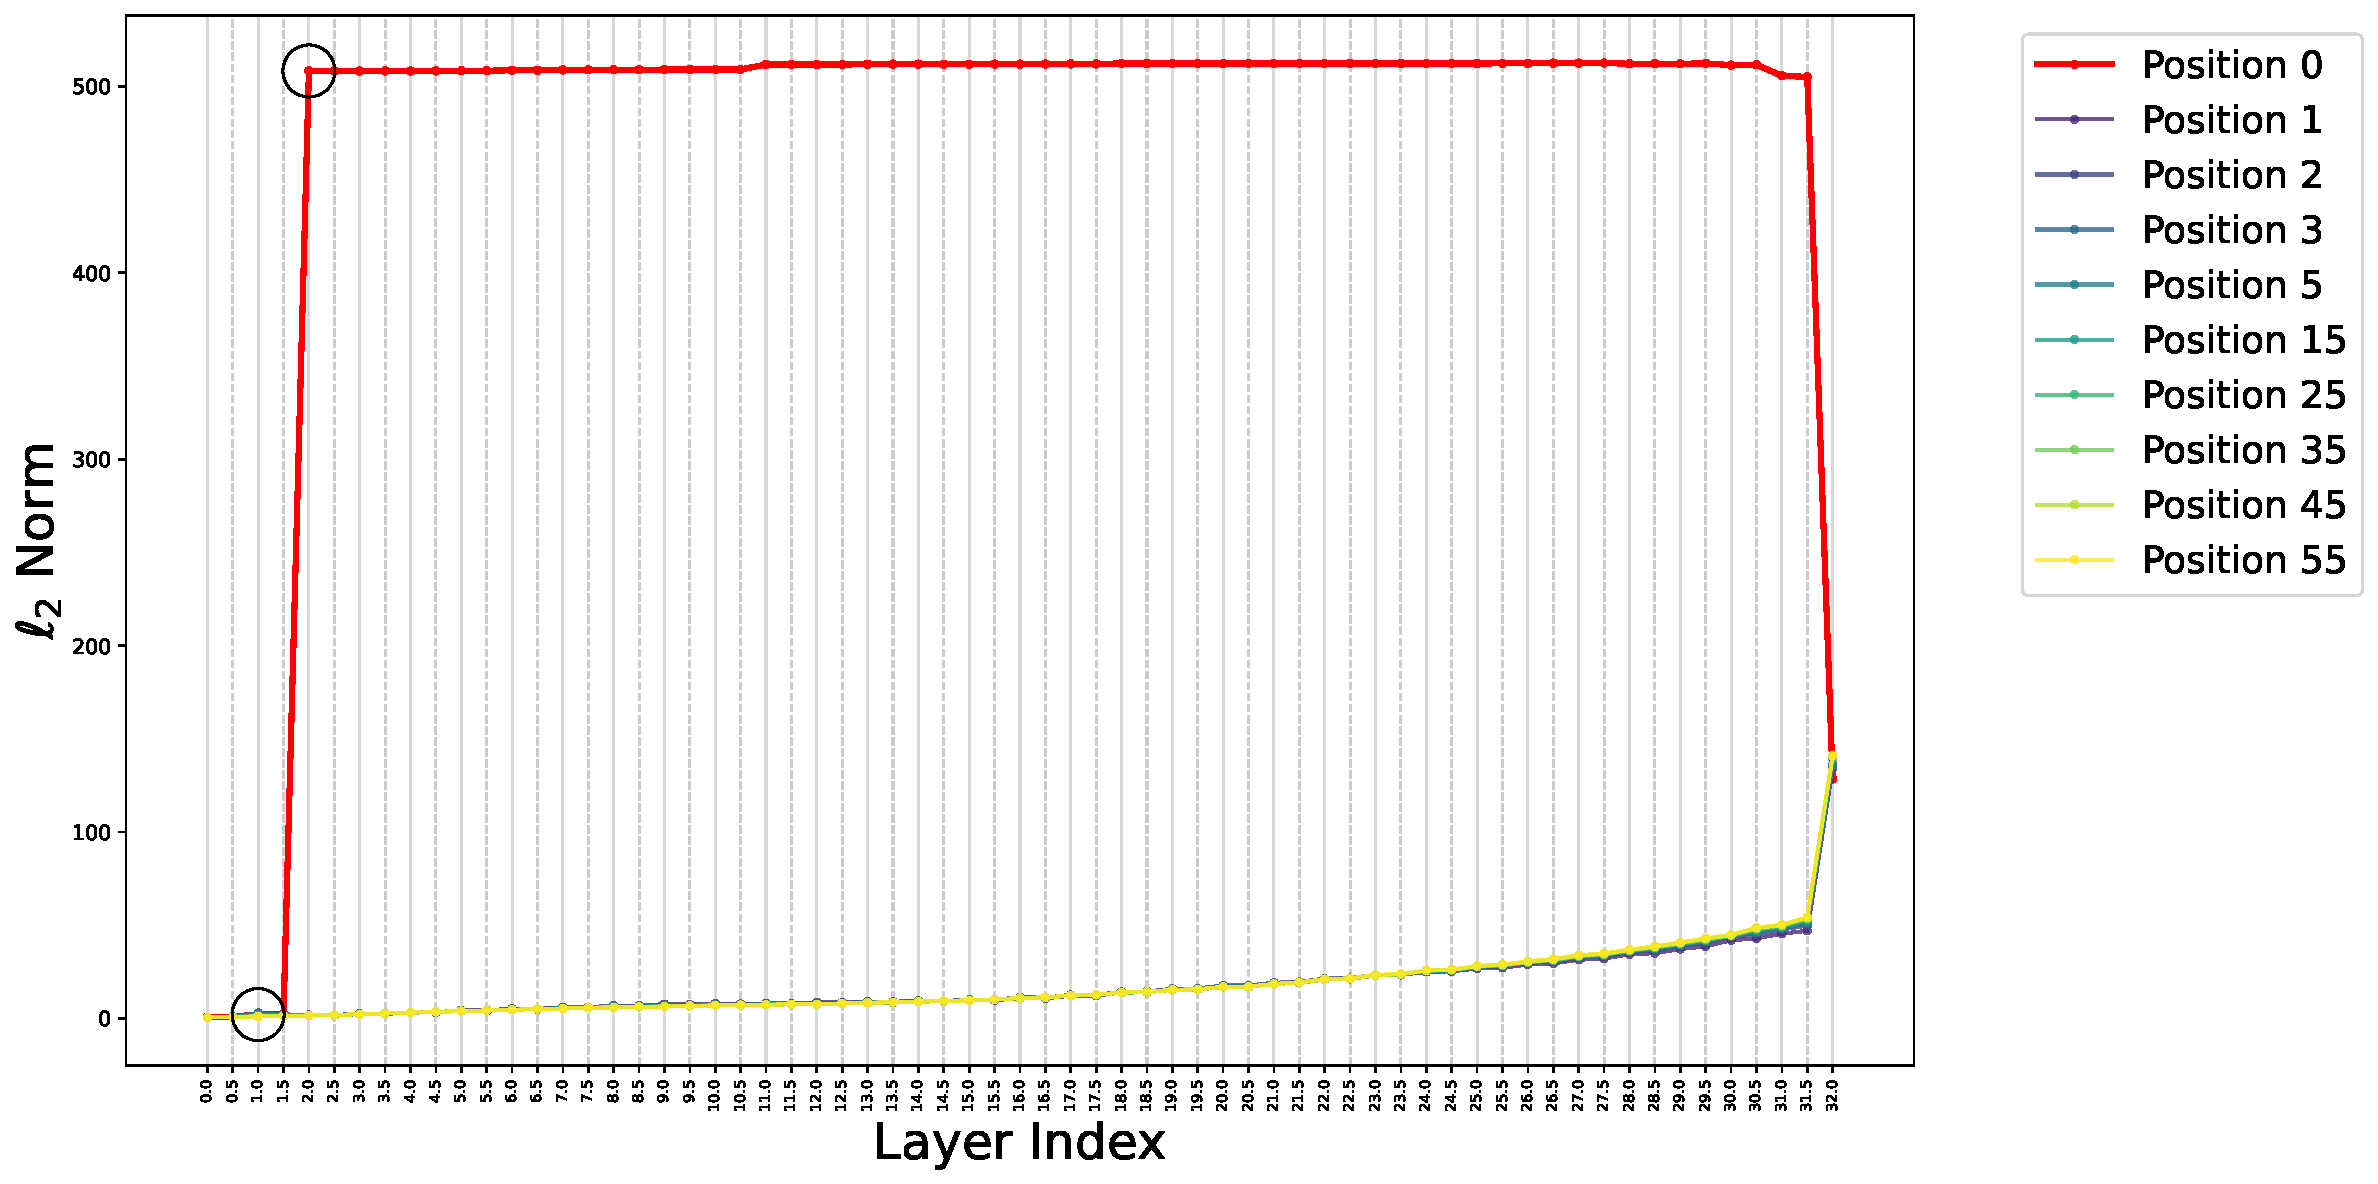
\includegraphics[width=0.95\columnwidth]{figures/fig2/fig2_2_llama_wo_bos.pdf}
%     \end{subfigure}
%     \begin{subfigure}[b]{0.18\linewidth} 
%         \centering
%         \begin{subfigure}[b]{\linewidth} 
%             \centering
%             \caption{\scriptsize{Layer 1 Average Attention Score}}
%             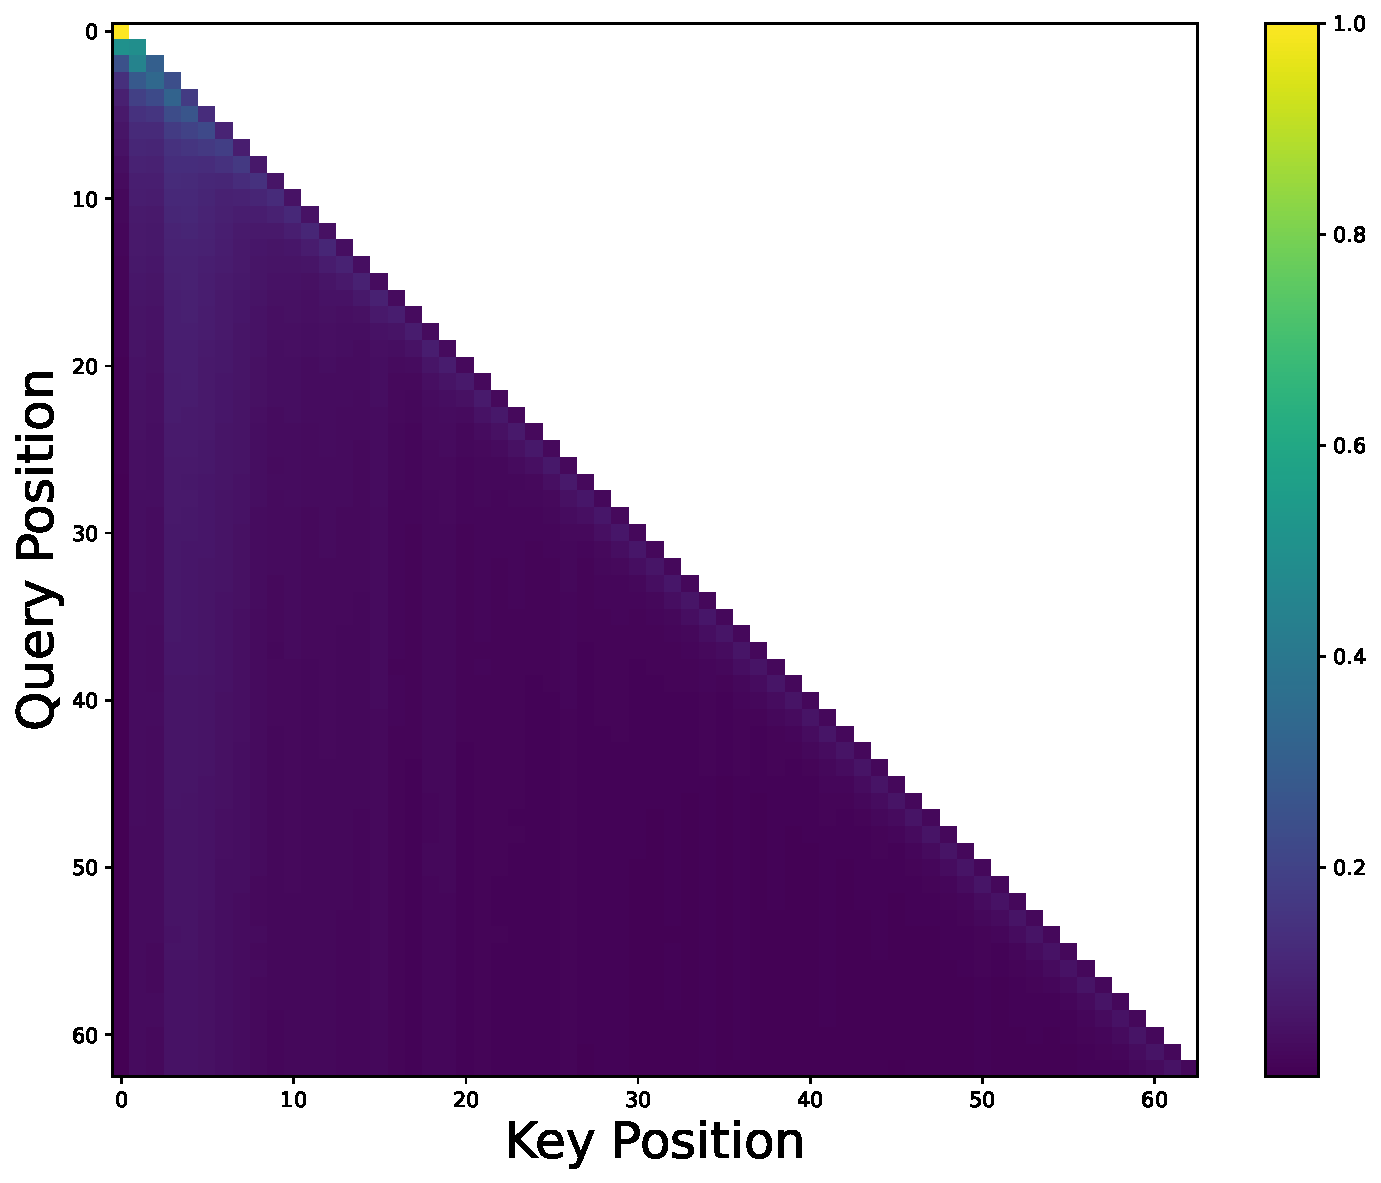
\includegraphics[width=\linewidth]{figures/fig2/fig2_1_llama_wo_bos_layer1.pdf}
%         \end{subfigure}
%         \begin{subfigure}[b]{\linewidth}
%             \centering
%             \caption{\scriptsize{Layer 2 Average Attention Score}} 
%             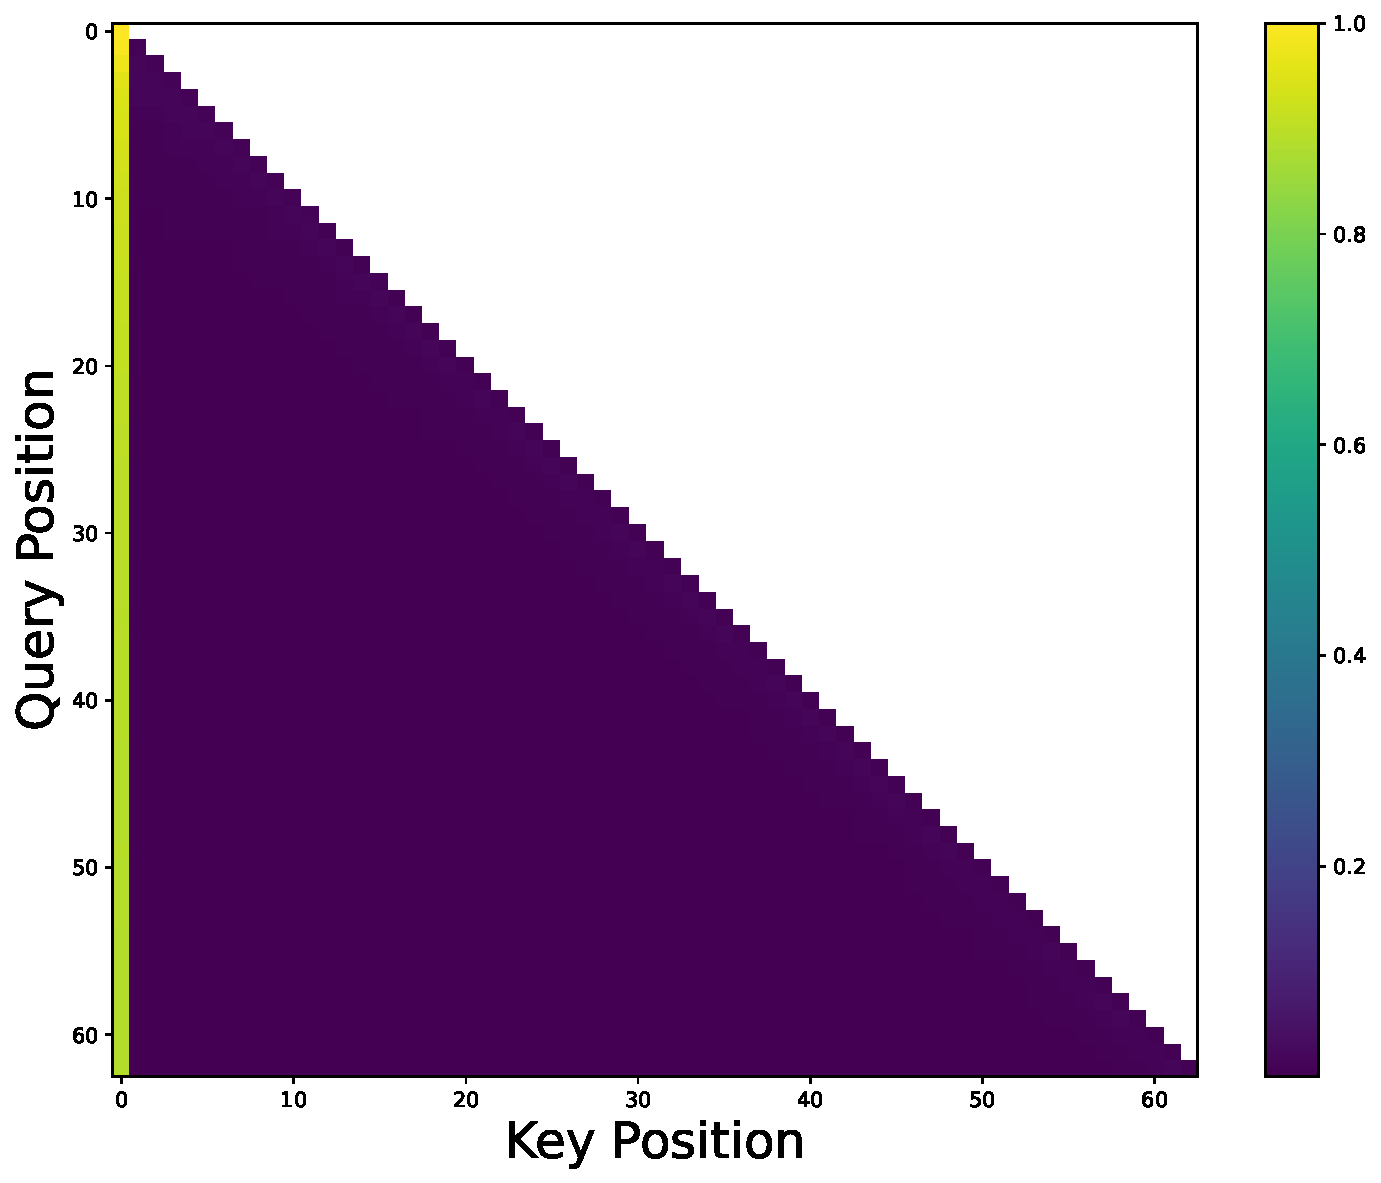
\includegraphics[width=\linewidth]{figures/fig2/fig2_1_llama_wo_bos_layer2.pdf}
%         \end{subfigure}
%     \end{subfigure}
% \end{minipage}
% \caption{The P0 sink is not solely caused by embedding of [BOS], but reflects a persistent circuit-level activation pattern.}
% \label{bos-vs-non-bos-fig1}
% \end{figure*}

% \begin{figure*}[t]
% \caption{The P0 sink pattern observed under repeated first-token inputs}
% \label{bos-vs-non-bos-fig2}
% \end{figure*}

% The foundation of this behavior lies in the use of non-additive positional encoding schemes. Modern LLMs have abandoned the original additive positional encodings \citep{NIPS2017_3f5ee243}, adopting instead design practices that support longer context windows and stronger extrapolation capabilities. Alternative approaches, such as relative positional encodings and rotary position embeddings, inject position information exclusively into the attention mechanism, leaving the MLP and residual pathways agnostic to positional order \citep{kazemnejad2023impactpositionalencodinglength, su2023roformerenhancedtransformerrotary, press2022trainshorttestlong}. As a result of this design choice, when the same token is repeated $n$ times at the beginning of a sequence, the hidden states of the first $n$ tokens become exactly identical \citep{gu2025attentionsinkemergeslanguage}. This symmetry in representations can lead to out-of-distribution (OOD) attention score patterns, where the model produces spurious or degenerate attention behaviors that do not reflect the true semantic structure of the input.

% \begin{takeawaysbox}
% \textbf{Takeaways:}
% \begin{enumerate}
%     \item LLMs exhibit P0 attention sink regardless of the presence of a [BOS] token.
%     \item The embedding of [BOS] contributes primarily to shallow-layer P0 attention sink.
%     \item Embedding-based attention sinks are more fragile under out-of-distribution (OOD) scenarios.
% \end{enumerate}
% \end{takeawaysbox}


% \section{The P0 Token Detection Circuit}

% Taking the LLaMA architecture as a representative example, we show that a minimal transformer subnetwork composed of two attention layers and two MLP layers is sufficient to implement a position-zero (P0) token identification circuit.

% The first attention layer applies a strong locality bias. Each token mainly attends to itself and a few preceding tokens, resulting in localized aggregation of contextual information. This operation mixes diverse representations for different tokens, which suppresses any shared directional component that could signal the identity of the P0 token. In contrast, the P0 token only attends to itself and therefore fully retains this component. This asymmetry introduces a representational distinction between P0 and non-P0 tokens in the output of the first attention module.

% The first MLP layer builds on this difference by amplifying the preserved component through its up-projection. Because the P0 token's input carries a stronger alignment with the relevant direction, its output becomes more concentrated along that axis. Non-P0 tokens, having already diluted this component, are affected to a much lesser extent.

% The second attention layer further strengthens this separation. Tokens that now encode the amplified component from P0 are more likely to focus attention back on P0, reinforcing its centrality in the representation. This recurrence makes the P0 direction increasingly prominent.

% Finally, the second MLP layer projects the already enhanced component into a high-magnitude vector aligned with a fixed direction in the representation space. The pre-normalization applied before this MLP operation emphasizes the linear component in the input, allowing the MLP to sharpen the separation even further.

% Through this sequence of four operations—two attention modules followed by two MLPs—the hidden state at position zero exhibits a significantly amplified $\ell_2$ norm. This observation is consistent with the findings of \citet{gu2025attentionsinkemergeslanguage}, where the P0 token is shown to maintain a stable and dominant representational role across layers, contributing directly to the formation of attention sinks.


\section{How LLMs Sink the Position-Zero Token}


\subsection{Fixed Representation at Position Zero}

Figure~\ref{bos-vs-non-bos-fig1} demonstrates that even after removing the \texttt{[BOS]} token from a model trained with it, the model still successfully localizes the position-zero (P0) token within just two transformer blocks. Notably, the MLP further amplifies the hidden state at this position by increasing its $\ell_2$ norm. Figure~\ref{8b_no_bos_cos_sim_fig} reveals that the MLP not only increases the magnitude, but also projects the P0 hidden state toward a consistent direction in the representation space.

This amplification brings two key benefits. First, it reduces the influence of token embeddings on the representation of position zero. Since the MLP output is added to the residual stream, the amplified hidden state at P0 dominates the combined representation, effectively suppressing earlier-layer contributions that are several orders of magnitude smaller.

Second, when combined with the pre-layer RMS normalization (pre-norm) commonly used in modern LLMs \citep{zhang2019rootmeansquarelayer, ba2016layernormalization}, the amplified norm helps stabilize the P0 representation during training. A high-magnitude vector is less sensitive to gradient updates and more likely to preserve its direction across optimization steps. This stability enables the model to maintain a consistent and distinguishable representation of P0 tokens throughout training.

\begin{figure*}[ht]
    \centering
        \begin{minipage}[b]{0.32\linewidth} 
        \centering
        \begin{subfigure}[b]{0.95\linewidth} 
            \centering
            \caption{\scriptsize{t-SNE of Layer 0 \\ MLP Intermediate States}}
            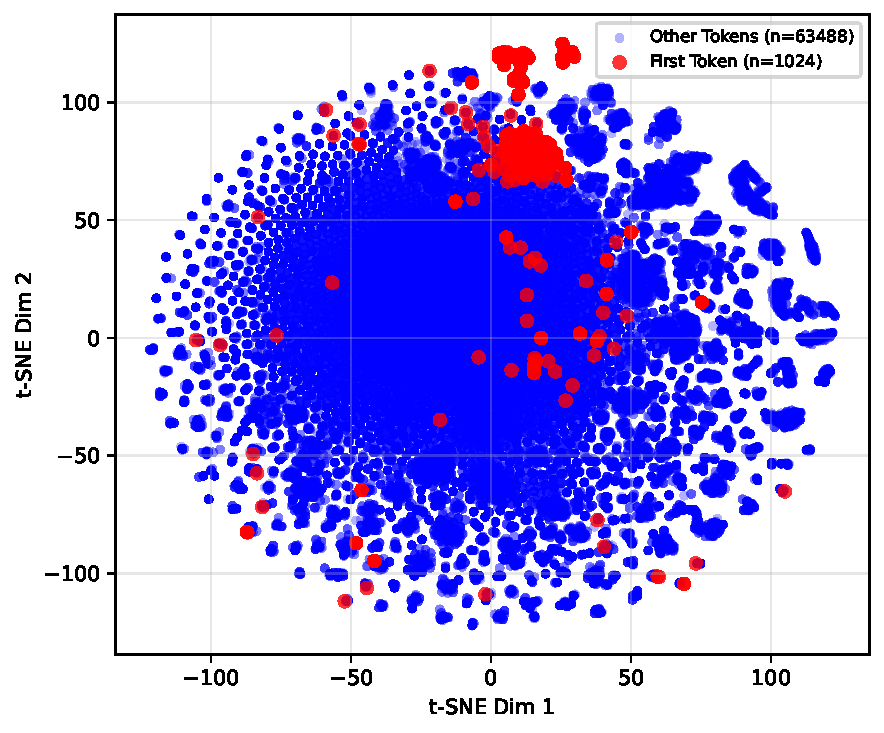
\includegraphics[width=0.95\columnwidth]{figures/fig3/fig3_tsne_layer0_llama3_1_8b.pdf}
        \end{subfigure}
        \begin{subfigure}[b]{0.95\linewidth} 
            \centering
            \caption{\scriptsize{Average Attention Scores \\ among Layer 0}}
            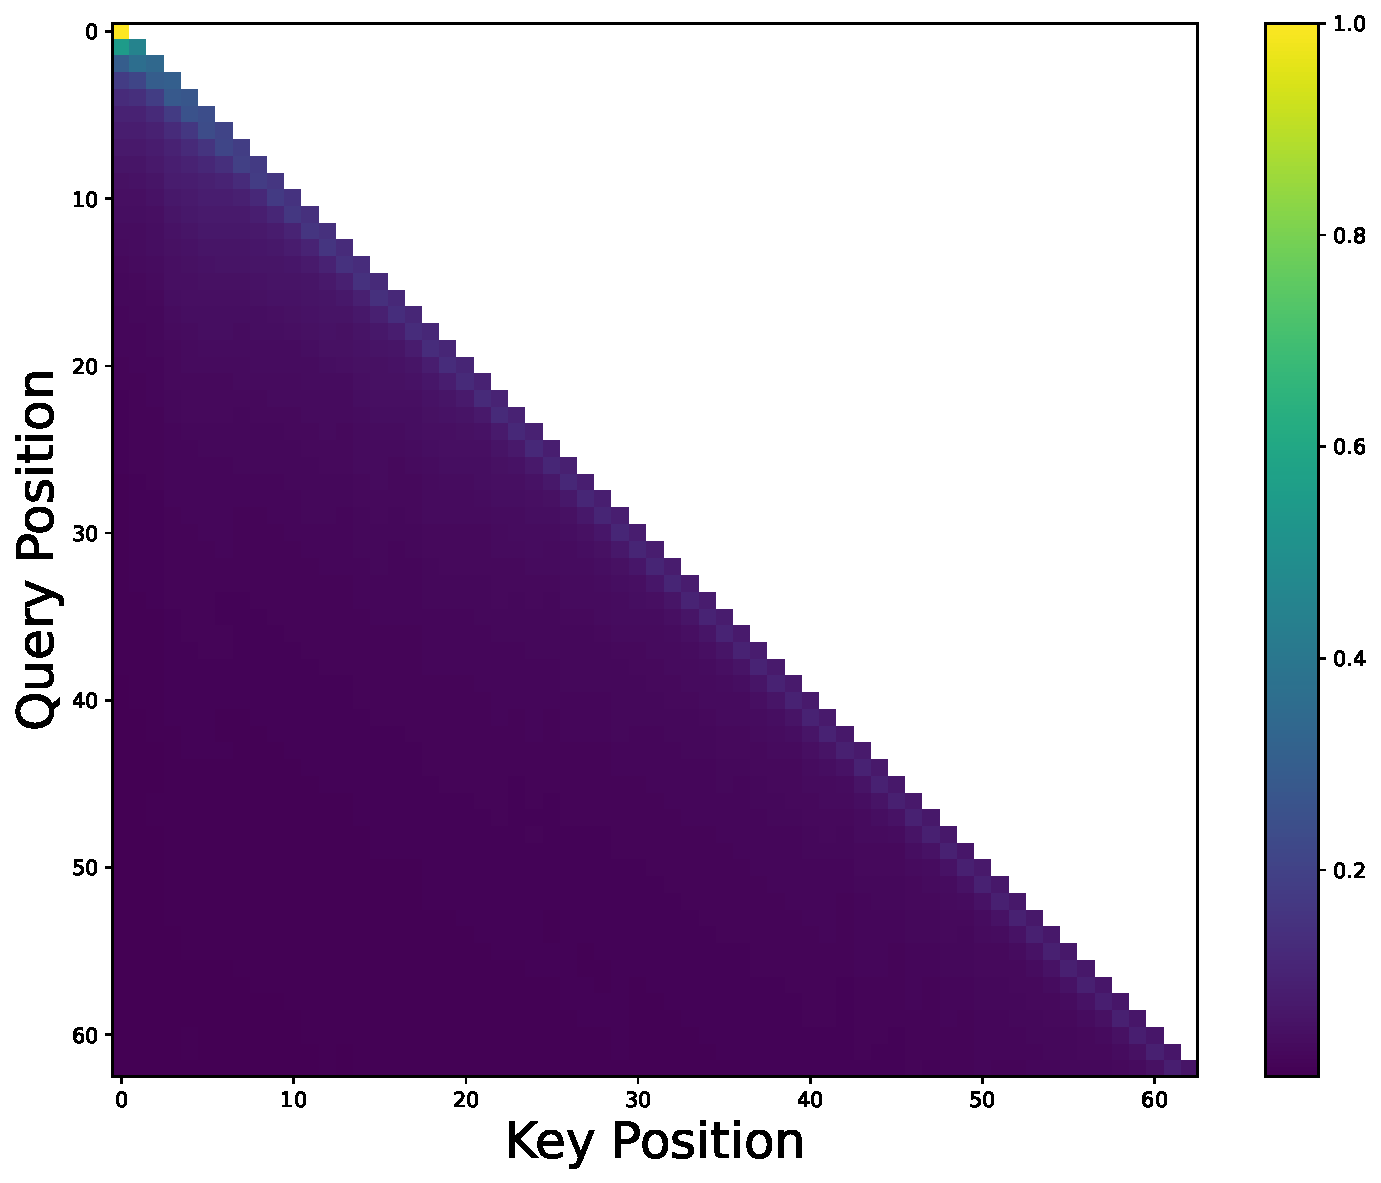
\includegraphics[width=0.95\columnwidth]{figures/fig3/fig3_llama3_1_8b_layer0_avg.pdf}
            \label{fig4-b}
        \end{subfigure}
    \end{minipage}
    \begin{minipage}[b]{0.32\linewidth} 
        \centering
        \begin{subfigure}[b]{0.95\linewidth} 
            \centering
            \caption{\scriptsize{t-SNE of Layer 0 MLP Intermediate States \\ w/o Head 2}}
            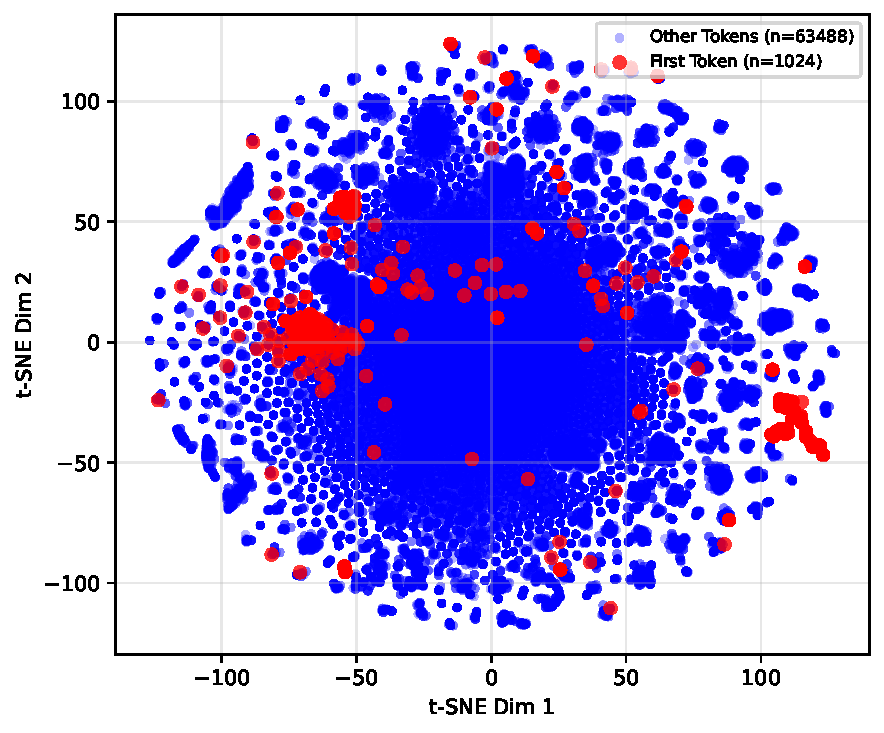
\includegraphics[width=0.95\columnwidth]{figures/fig3/fig3_tsne_layer0_llama3_1_8b_ablation_head2.pdf}
            \label{fig4-c}
        \end{subfigure}
        \begin{subfigure}[b]{0.95\linewidth} 
            \centering
            \caption{\scriptsize{Attention Scores \\ of Removed Layer 0 Head 2}}
            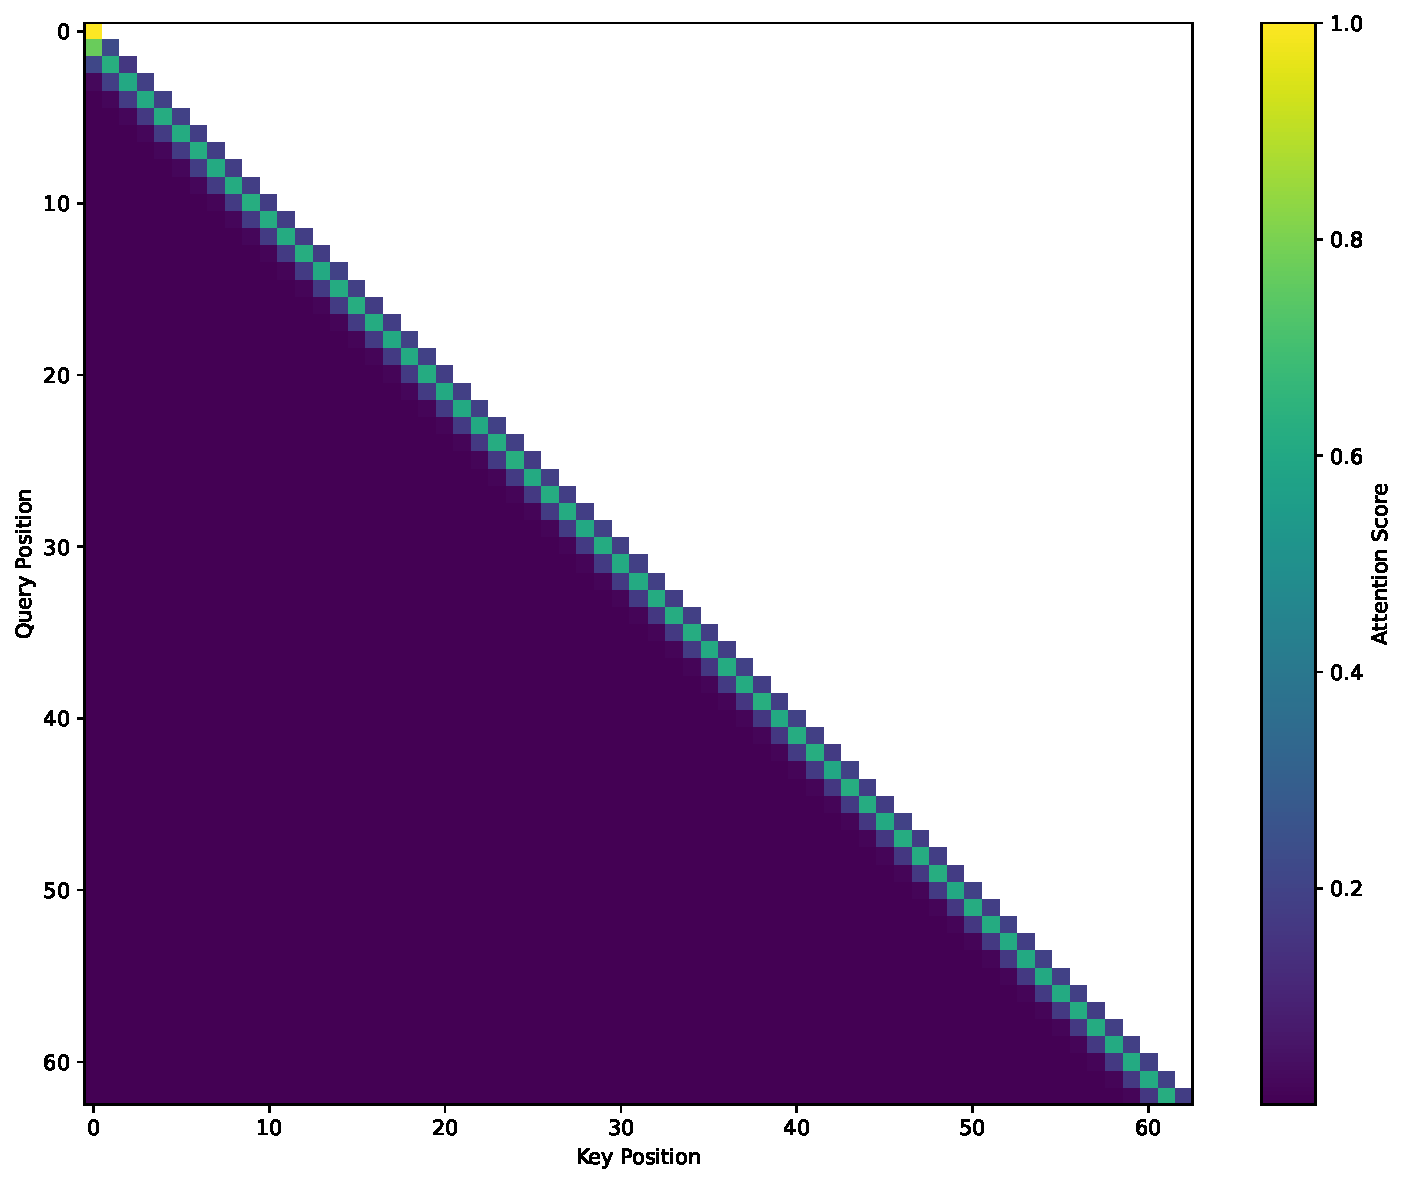
\includegraphics[width=0.95\columnwidth]{figures/fig3/fig3_llama3_1_8b_layer0_head2_attention.pdf}
            \label{fig4-d}
        \end{subfigure}
    \end{minipage}
    \begin{minipage}[b]{0.32\linewidth} 
        \centering
        \begin{subfigure}[b]{0.95\linewidth} 
            \centering
            \caption{\scriptsize{t-SNE of Layer 0 MLP Intermediate States \\  w/o Head 29}}
            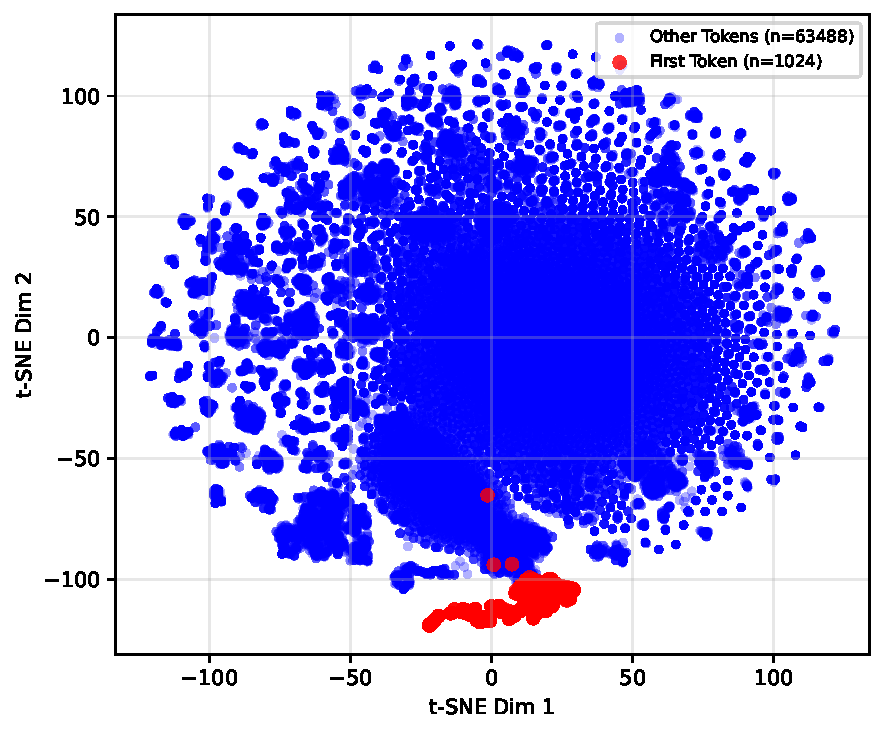
\includegraphics[width=0.95\columnwidth]{figures/fig3/fig3_tsne_layer0_llama3_1_8b_ablation_head29.pdf}
        \end{subfigure}
        \begin{subfigure}[b]{0.95\linewidth} 
            \centering
            \caption{\scriptsize{Attention Scores \\ of Removed Layer 0 Head 29}}
            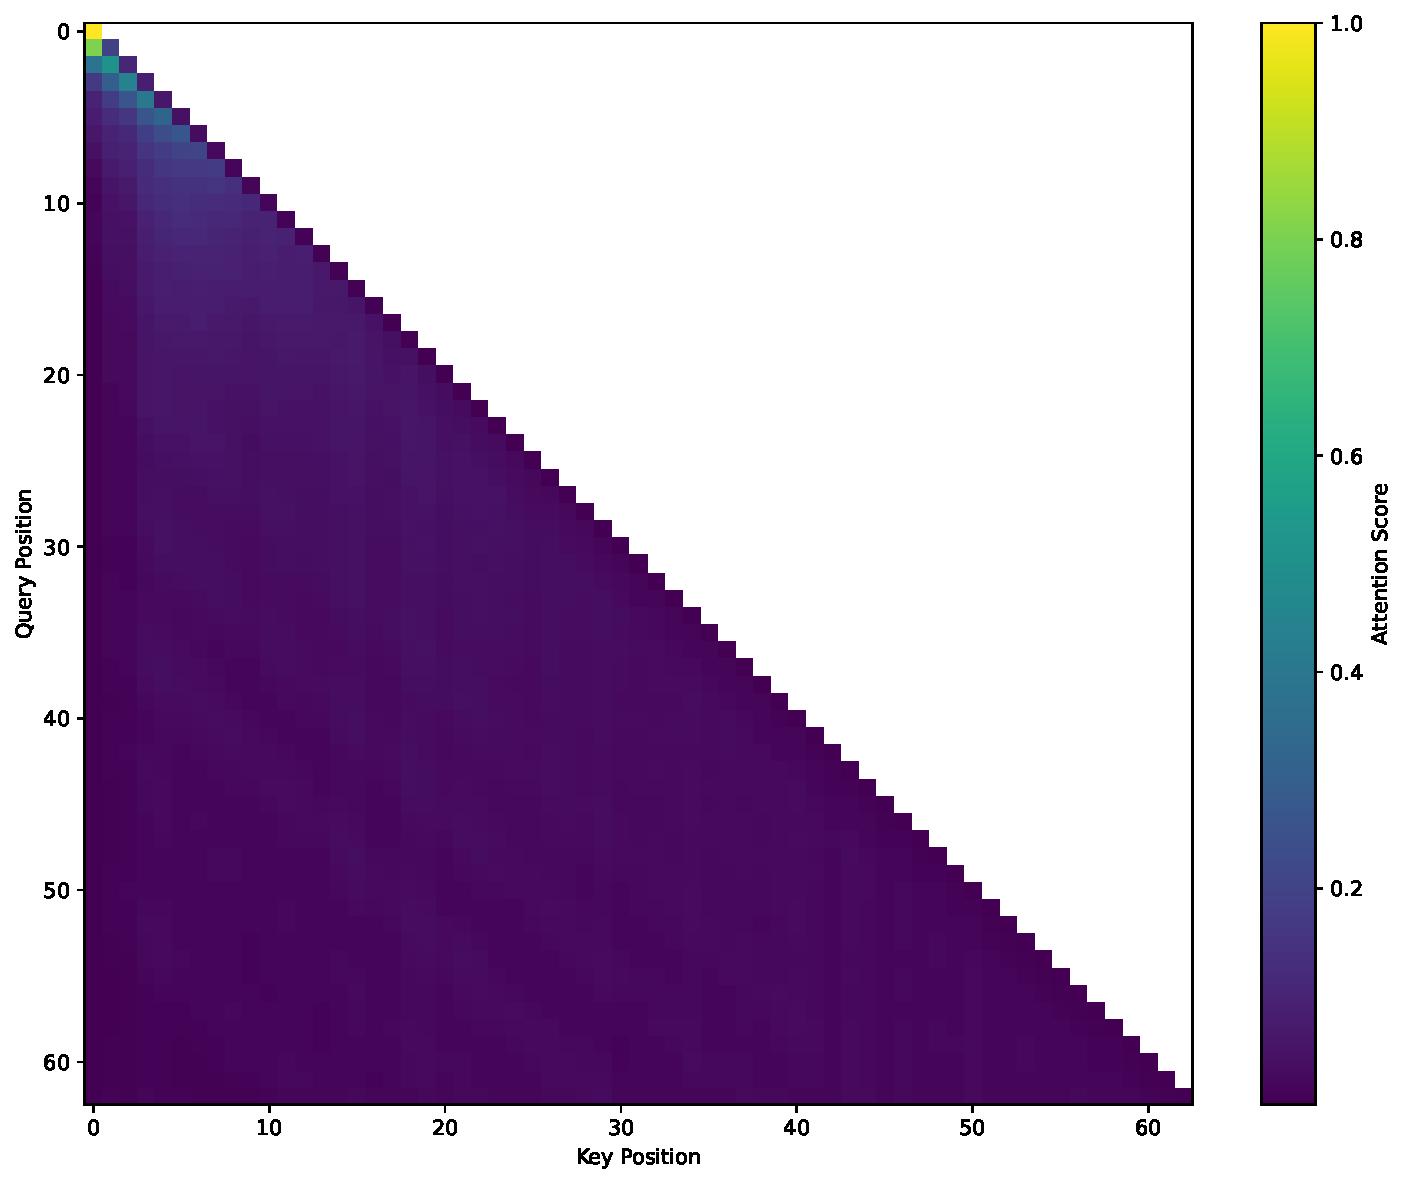
\includegraphics[width=0.95\columnwidth]{figures/fig3/fig3_llama3_1_8b_layer0_head29_attention.pdf}
        \end{subfigure}
    \end{minipage}
    \caption{Visualization of intermediate MLP activations and attention scores in layer 0 of LLaMA3.1-8B. The \texttt{[BOS]} token has been removed. Several heads exhibit strong locality by primarily attending to neighboring tokens. Ablating individual heads does not weaken the clustering behavior at position zero; in fact, removing certain heads can even enhance it. This suggests that the effect arises from a complex, collaborative mechanism involving multiple attention heads.}
    \label{max_among_head_locality_fig}
    % \vspace{-2em}
\end{figure*}

\begin{figure}[ht]
    \centering
    \begin{minipage}[b]{0.94\linewidth} 
        \begin{subfigure}[b]{0.47\linewidth} 
            \centering
            \caption{\scriptsize{PCA of Layer 1 MLP Input}}
            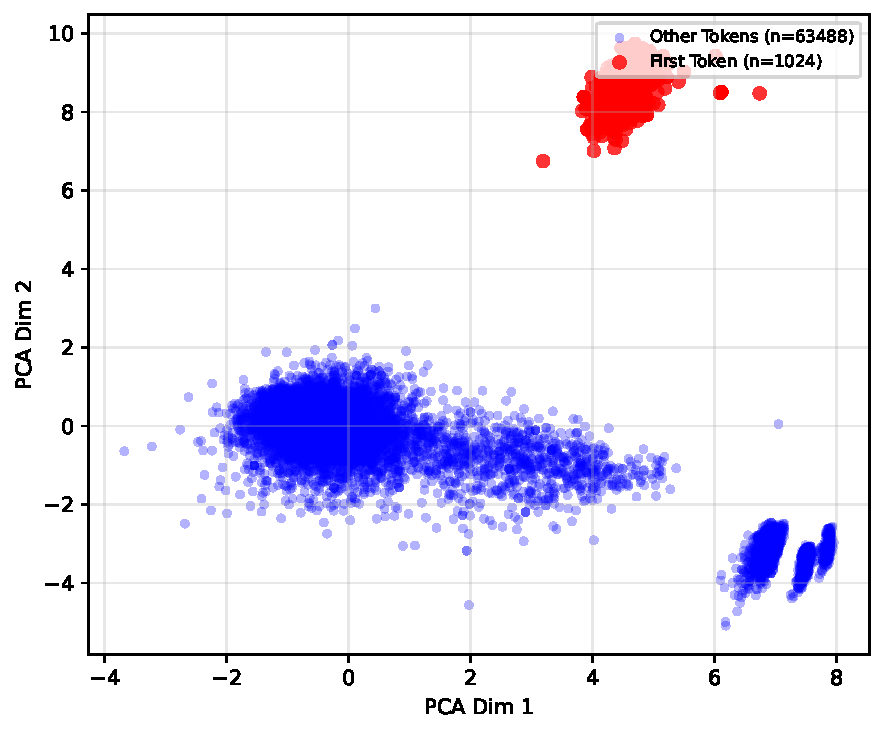
\includegraphics[width=\linewidth]{figures/fig5/fig5_llama3_1_8b_no_bos_layer1_5_pca.pdf}
        \end{subfigure}
        \begin{subfigure}[b]{0.47\linewidth}
            \centering
            \caption{\scriptsize{PCA of Layer 2 Attn Input}} 
            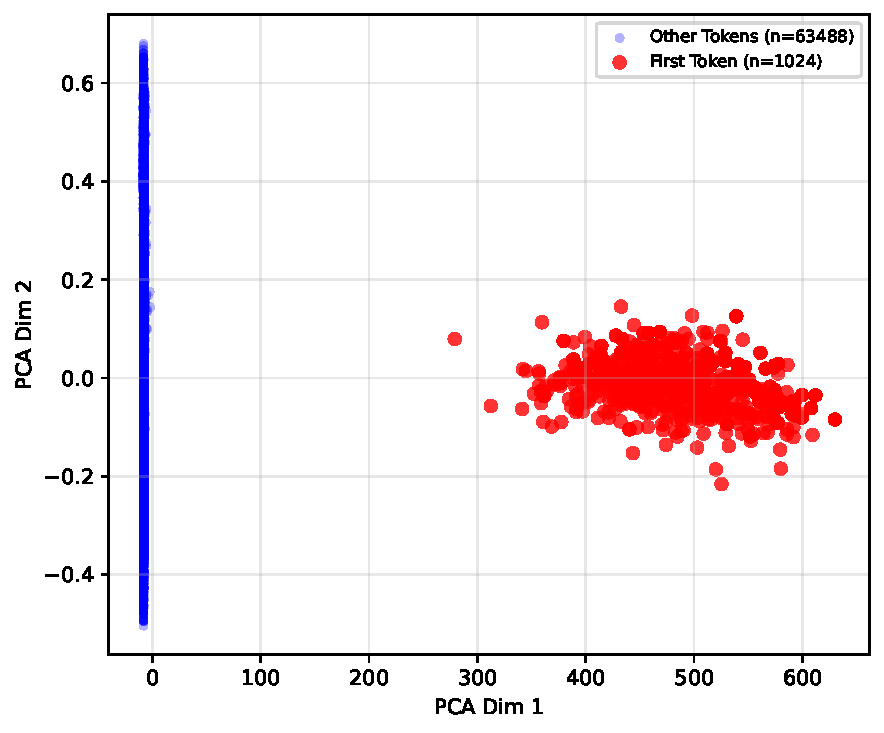
\includegraphics[width=\linewidth]{figures/fig5/fig5_llama3_1_8b_no_bos_layer2_pca.pdf}
        \end{subfigure}
        \vspace{-0.5em}
        \caption{PCA of hidden states after the corresponding pre-layer normalization in LLaMA3.1-8B, with \texttt{[BOS]} token removed.}
        \label{fig-amp-llama3-8b}
    \end{minipage}
    % \vspace{-2em}
\end{figure}

To better formalize the model’s behavior in constructing a consistent and distinguishable representation for position-zero (P0), we begin by examining the pre-norm transformation applied to a hidden state vector $\mathbf{x} \in \mathbb{R}^d$, which precedes any downstream neural network module:
\begin{equation}
    \text{Norm}(\mathbf{x}) = \frac{\mathbf{x}}{r(\mathbf{x})},
\end{equation}
where the norm factor is defined as
\begin{equation}
    r(\mathbf{x}) = {\sqrt{\frac{1}{d} \mathbf{x}^\top \mathbf{x}}}.
\end{equation}

The Jacobian of this operation with respect to $\mathbf{x}$ is given by:
\begin{equation}
    \mathbf{J}_{\text{Norm}}(\mathbf{x}) = \frac{1}{r(\mathbf{x})} \mathbf{I} - \frac{1}{d} \frac{1}{r^3(\mathbf{x})} \mathbf{x} \mathbf{x}^\top.
\end{equation}

Now consider a perturbation to the hidden state $\delta \mathbf{x} \ll \mathbf{x}$ induced by a backward update during training. This perturbation can be decomposed into components parallel and orthogonal to $\mathbf{x}$:
\begin{equation}
    \delta \mathbf{x} = \delta \mathbf{x}_\parallel + \delta \mathbf{x}_\perp, \text{where } \delta \mathbf{x}_\parallel = \alpha \mathbf{x}, \delta \mathbf{x}_\perp \cdot \mathbf{x} = 0.
\end{equation}
The change in the normalized vector is approximately:
\begin{equation}
    \text{Norm}(\mathbf{x} + \delta \mathbf{x}) - \text{Norm}(\mathbf{x}) \approx \mathbf{J}_{\text{Norm}}(\mathbf{x})\delta\mathbf{x}  =  \frac{\delta \mathbf{x}_\perp}{r(\mathbf{x})} .
    \label{eq:norm}
\end{equation}

This expression leads to a key insight: when $r(\mathbf{x})$ is large, the effect of orthogonal perturbations $\delta \mathbf{x}_\perp$ on the normalized vector becomes proportionally smaller. Under the standard i.i.d. assumption on training data, gradient noise can be treated as approximately independent of the input. Thus, increasing the norm of $\mathbf{x}$ reduces the sensitivity of its normalized direction to parameter updates.

% Furthermore, this stabilization imposes an implicit constraint on the form of the representation. To preserve a fixed and robust direction across diverse inputs and training updates, the hidden state at position zero benefits from being disentangled from the input content. Ideally, it should encode position-specific information while remaining invariant to the actual token identity. 

\subsection{Position Zero Identification Circuit}

We now turn to how the model establishes the positional signature before the amplification phase. Empirically, the distinction of the first token is already visible in the hidden states after layer 0, where the position-zero representation is consistently pushed toward a relatively stable direction across inputs. This indicates that the model has already created a position-dependent asymmetry in the attention output prior to any strong MLP amplification. Additional evidence from Figure~\ref{fig-amp-llama3-8b} confirms that this identification is already established before the MLP in layer 1, which corresponds to the model’s second transformer block.

As illustrated in Figure~\ref{fig4-d}, several attention heads in layer 0 exhibit strong locality. While this pattern might initially seem relevant to the emergence of the position-zero (P0) sink, head-level ablation studies suggest otherwise. In particular, the t-SNE visualization on head-level ablation~\citep{cai2022theoreticalfoundationstsnevisualizing} in Figure~\ref{max_among_head_locality_fig} shows that these local heads do not play a central role in producing the effect. Instead, the position-zero asymmetry arises from the collective behavior of attention heads that distribute attention broadly and evenly across the sequence, following a statistically uniform averaging pattern. This effect appears to result from their coordinated interactions rather than from the influence of any individual head. Furthermore, as shown in Figure~\ref{fig4-b}, local heads contribute only marginally to the average attention scores. For these reasons, we focus our analysis on the aggregate behavior of the non-local attention heads.

Intuitively, under the causal constraint, uniform averaging induces an inherent asymmetry between position zero and all later positions. Tokens at all later positions aggregate diverse context vectors, which reduces the consistency of any shared directional component in their attention outputs. In contrast, position zero has access only to itself, so its attention output remains unmixed and preserves its direction more reliably. This asymmetry provides a clean signal that subsequent MLP sublayers can gate and amplify, eventually producing a stable P0 representation and the corresponding sink pattern.

% Motivated by this observation, we proceed with a simplified analysis of the model by assuming that the input to the attention module is given by $\mathbf{x} = \mathbf{x}_0, \dots, \mathbf{x}_{l-1}$, where each vector has unit norm as a result of pre-layer normalization; that is, $|\mathbf{x}_i|_2 = 1$ for all $i$.

Motivated by the empirical observation that uniform averaging heads play a crucial role in forming the P0 sink, we develop a simplified model to theoretically estimate the norm of the attention output. We assume that the input vectors to the attention module $\mathbf{x} = \mathbf{x}_0, \dots, \mathbf{x}_{l-1}$ have been normalized to unit norm due to pre-layer normalization, i.e., $\|\mathbf{x}_i\|_2 = 1$ for all $i$.
Rather than modeling the detailed mechanism of attention, we abstract it as a weighted sum over value vectors $\mathbf{v}_0, \dots, \mathbf{v}_{l-1}$ using attention weights $\mathbf{p} = (p_0, \dots, p_{l-1})$. 
% We assume $\mathbf{p} = \mathrm{softmax}(\mathbf{z})$ with $\mathbf{z} \sim \mathcal{N}(\mathbf{0}, \sigma^2 \mathbf{I})$, so that by permutation symmetry, $\mathbb{E}[p_i] = 1/l$.

\paragraph{Cone-based model of value vectors.}
As shown in Figure~\ref{8b_no_bos_cos_sim_fig}, the hidden states in LLMs exhibit clear directional bias and are far from isotropic. To capture this phenomenon, we model the value vectors $\mathbf{v}_i$ as lying on a fixed-angle cone centered around a unit vector $\mathbf{u} \in \mathbb{R}^d$ , where pre-norm normalization ensures $\|\mathbf{v}_i\|_2 = 1$. Figure~\ref{8b_no_bos_cos_sim_fig} illustrates the cosine similarity structure. Each $\mathbf{v}_i$ is assumed to have unit norm and to form a constant cosine similarity $\alpha$ with the cone axis $\mathbf{u}$. A convenient construction of such vectors is:
\begin{equation}
\mathbf{v}_i = \alpha \mathbf{u} + \sqrt{1 - \alpha^2} \, \mathbf{s}_i,
\end{equation}
where each $\mathbf{s}_i$ is a unit vector orthogonal to $\mathbf{u}$, sampled uniformly from the $(d-1)$-dimensional unit sphere, and independent across $i$.

Under this construction, it follows that:
\begin{equation}
\mathbb{E}[\mathbf{v}_i^\top \mathbf{v}_j] = 
\begin{cases}
1, & i = j, \\
\alpha^2, & i \neq j.
\end{cases}
\end{equation}

\paragraph{Attention output norm.}  
Define the attention output of position $l-1$ as the weighted sum $\mathbf{c}$:
\begin{equation}
\mathbf{c} = \sum_{i=0}^{l-1} p_i \mathbf{v}_i.
\end{equation}
We aim to estimate its expected squared norm $\mathbb{E}[\|\mathbf{c}\|_2^2]$. First, expand the square:
\begin{equation}
\|\mathbf{c}\|_2^2 = \sum_i p_i^2 \|\mathbf{v}_i\|_2^2 + \sum_{i \ne j} p_i p_j \mathbf{v}_i^\top \mathbf{v}_j.
\end{equation}
Taking expectation over $\mathbf{v}$ conditioned on $\mathbf{p}$, and substituting in the known moments:
\begin{align}
\mathbb{E}_{\mathbf{v}}[\|\mathbf{c}\|_2^2 \mid \mathbf{p}]
&= \sum_i p_i^2 \cdot 1 + \sum_{i \ne j} p_i p_j \cdot \alpha^2 \notag \\
&= \sum_i p_i^2 + \alpha^2 \left( 1 - \sum_i p_i^2 \right) \notag \\
&= \alpha^2 + (1 - \alpha^2) \sum_i p_i^2.
\end{align}
Finally, taking expectation over $\mathbf{p}$ gives:
\begin{equation}
\mathbb{E}[\|\mathbf{c}\|_2^2]
= \alpha^2 + (1 - \alpha^2)\, \mathbb{E}\left[\sum_i p_i^2\right].
\label{eq:mixing}
\end{equation}

While the full distribution of attention weights $\mathbf{p}$ is difficult to characterize analytically, empirical observations suggest that attention tends to be sparse across positions~\citep{zucchet2025the}. This sparsity implies that the second-order statistic $\mathbb{E}\left[\sum_i p_i^2\right]$ typically decreases monotonically as the sequence length $l$ increases. This theoretical behavior aligns with our empirical finding that the $\ell_2$ norm of the attention output decreases with increasing sequence length $l$, as shown in Table~\ref{non-bos-l2norm-attnout-tab}.

Specifically, to ensure that our assumption is not confounded by the out-of-distribution effect caused by repeated contiguous tokens, as discussed in Section~\ref{sec2}, we verify the proportion of $n$-grams in which the same token appears $n$ times consecutively under different tokenizers. The results, summarized in Table~\ref{bos-vs-non-bos-tab2}, show that such occurrences are rare across common tokenizers. This confirms that the simultaneous occurrence of identical tokens at both position zero and position one is highly unlikely in practice, which further justifies that training without a \texttt{[BOS]} token does not introduce significant ambiguity.

\begin{table}[t]
\resizebox{\linewidth}{!}{
\begin{tabular}{lcccccccc}
\toprule
\textbf{Token Index}           & 0    & 1    & 2    & 4    & 8    & 16   & 32   & 64    \\
\midrule
\textbf{Llama-3.1-8B} & 0.87 & 0.82 & 0.79 & 0.73 & 0.66 & 0.63 & 0.61 & 0.59  \\
\textbf{Llama-3.2-1B} & 1.04 & 1.03 & 0.98 & 0.96 & 0.91 & 0.90 & 0.88 & 0.87  \\
\textbf{Llama-3.2-3B} & 1.37 & 1.29 & 1.21 & 1.17 & 1.11 & 1.10 & 1.07 & 1.05  \\
\bottomrule
\end{tabular}
}
\caption{$\ell_2$ Norm of Layer 0 Attention Output, w/o \texttt{[BOS]}}
\label{non-bos-l2norm-attnout-tab}
% % \vspace{-2em}
\end{table}

\begin{table}[t]
\resizebox{\linewidth}{!}{
\begin{tabular}{lccc}
\toprule
\textbf{Token Repeat Time (n) }   & n=2      & n=3      & n=4      \\
\midrule
\textbf{Llama-3 Tokenizer}     & 2.01$\times10^{-4}$ & 6.10$\times10^{-5}$ & 2.90$\times10^{-5}$ \\
\textbf{Mistral-v0.3 Tokenizer} & 4.12$\times10^{-3}$ & 6.28$\times10^{-4}$ & 5.90$\times10^{-5}$ \\
\textbf{Qwen3 Tokenizer}       & 4.52$\times10^{-3}$ & 6.88$\times10^{-4}$ & 6.00$\times10^{-5}$ \\
\bottomrule
\end{tabular}}
\caption{Proportion of $n$-grams in which the same token appears $n$ times consecutively, measured under different tokenizers on a subset of FineWeb-Edu 10B dataset~\citep{lozhkov2024fineweb-edu}. This analysis confirms that repeated-token patterns are rare and are unlikely to introduce out-of-distribution artifacts that could confound our findings.}
\label{bos-vs-non-bos-tab2}
% % \vspace{-2em}
\end{table}

Leveraging this distributional asymmetry, the model is able to cluster the hidden states at position zero using only the up-projection components of the MLP, without incorporating any semantic information. The activation function serves as a gating mechanism, allowing the subsequent MLP layer to transform the resulting vector into a stable and position-specific representation. Together, these components constitute what we refer to as the \textbf{P0-Sink Circuit}.


\section{How P0 Sink Emerges in Pre-training}

% \begin{figure}[t]
%     \centering
%     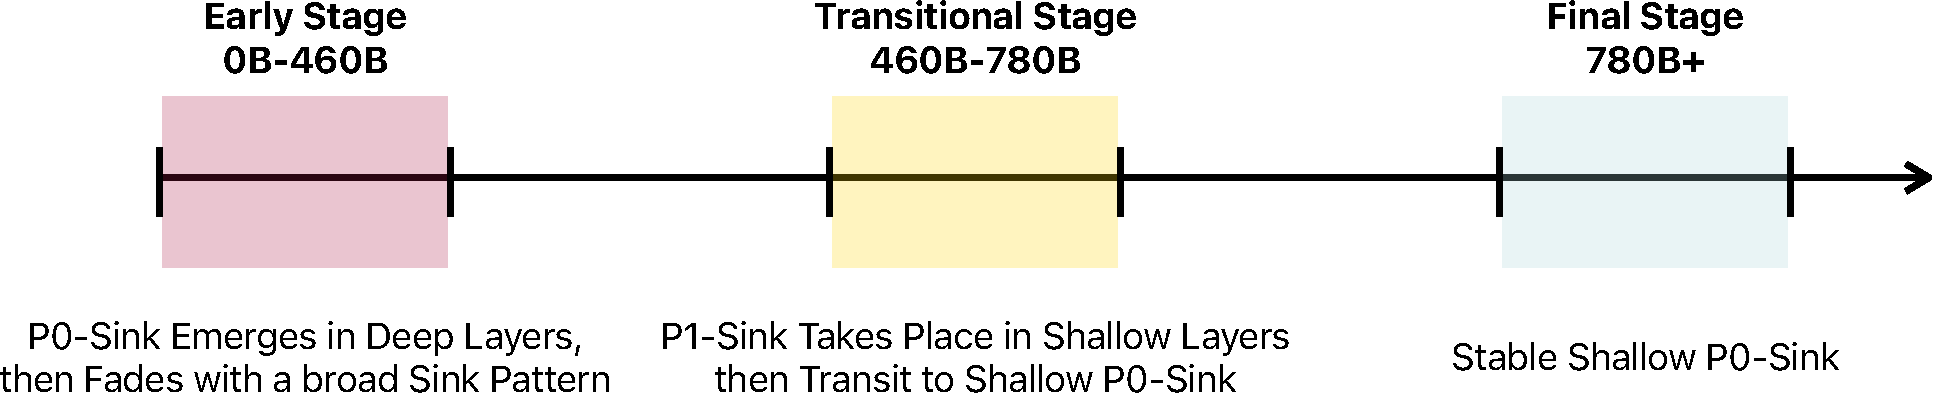
\includegraphics[width=0.95\linewidth]{figures/fig8/Fig8-cropped.pdf}
%     \caption{Illustration of Training Stages}
%     \label{fig-overall}
%     \vspace{-1em}
% \end{figure}

\begin{figure*}[ht]
\centering

\begin{minipage}[b]{0.32\linewidth} 
    \centering
    \begin{subfigure}[b]{0.95\linewidth} 
        \centering
        \caption{\scriptsize{Hidden States $\ell_2$Norm \\ Step 2000 ($\sim$15B Token)}}
        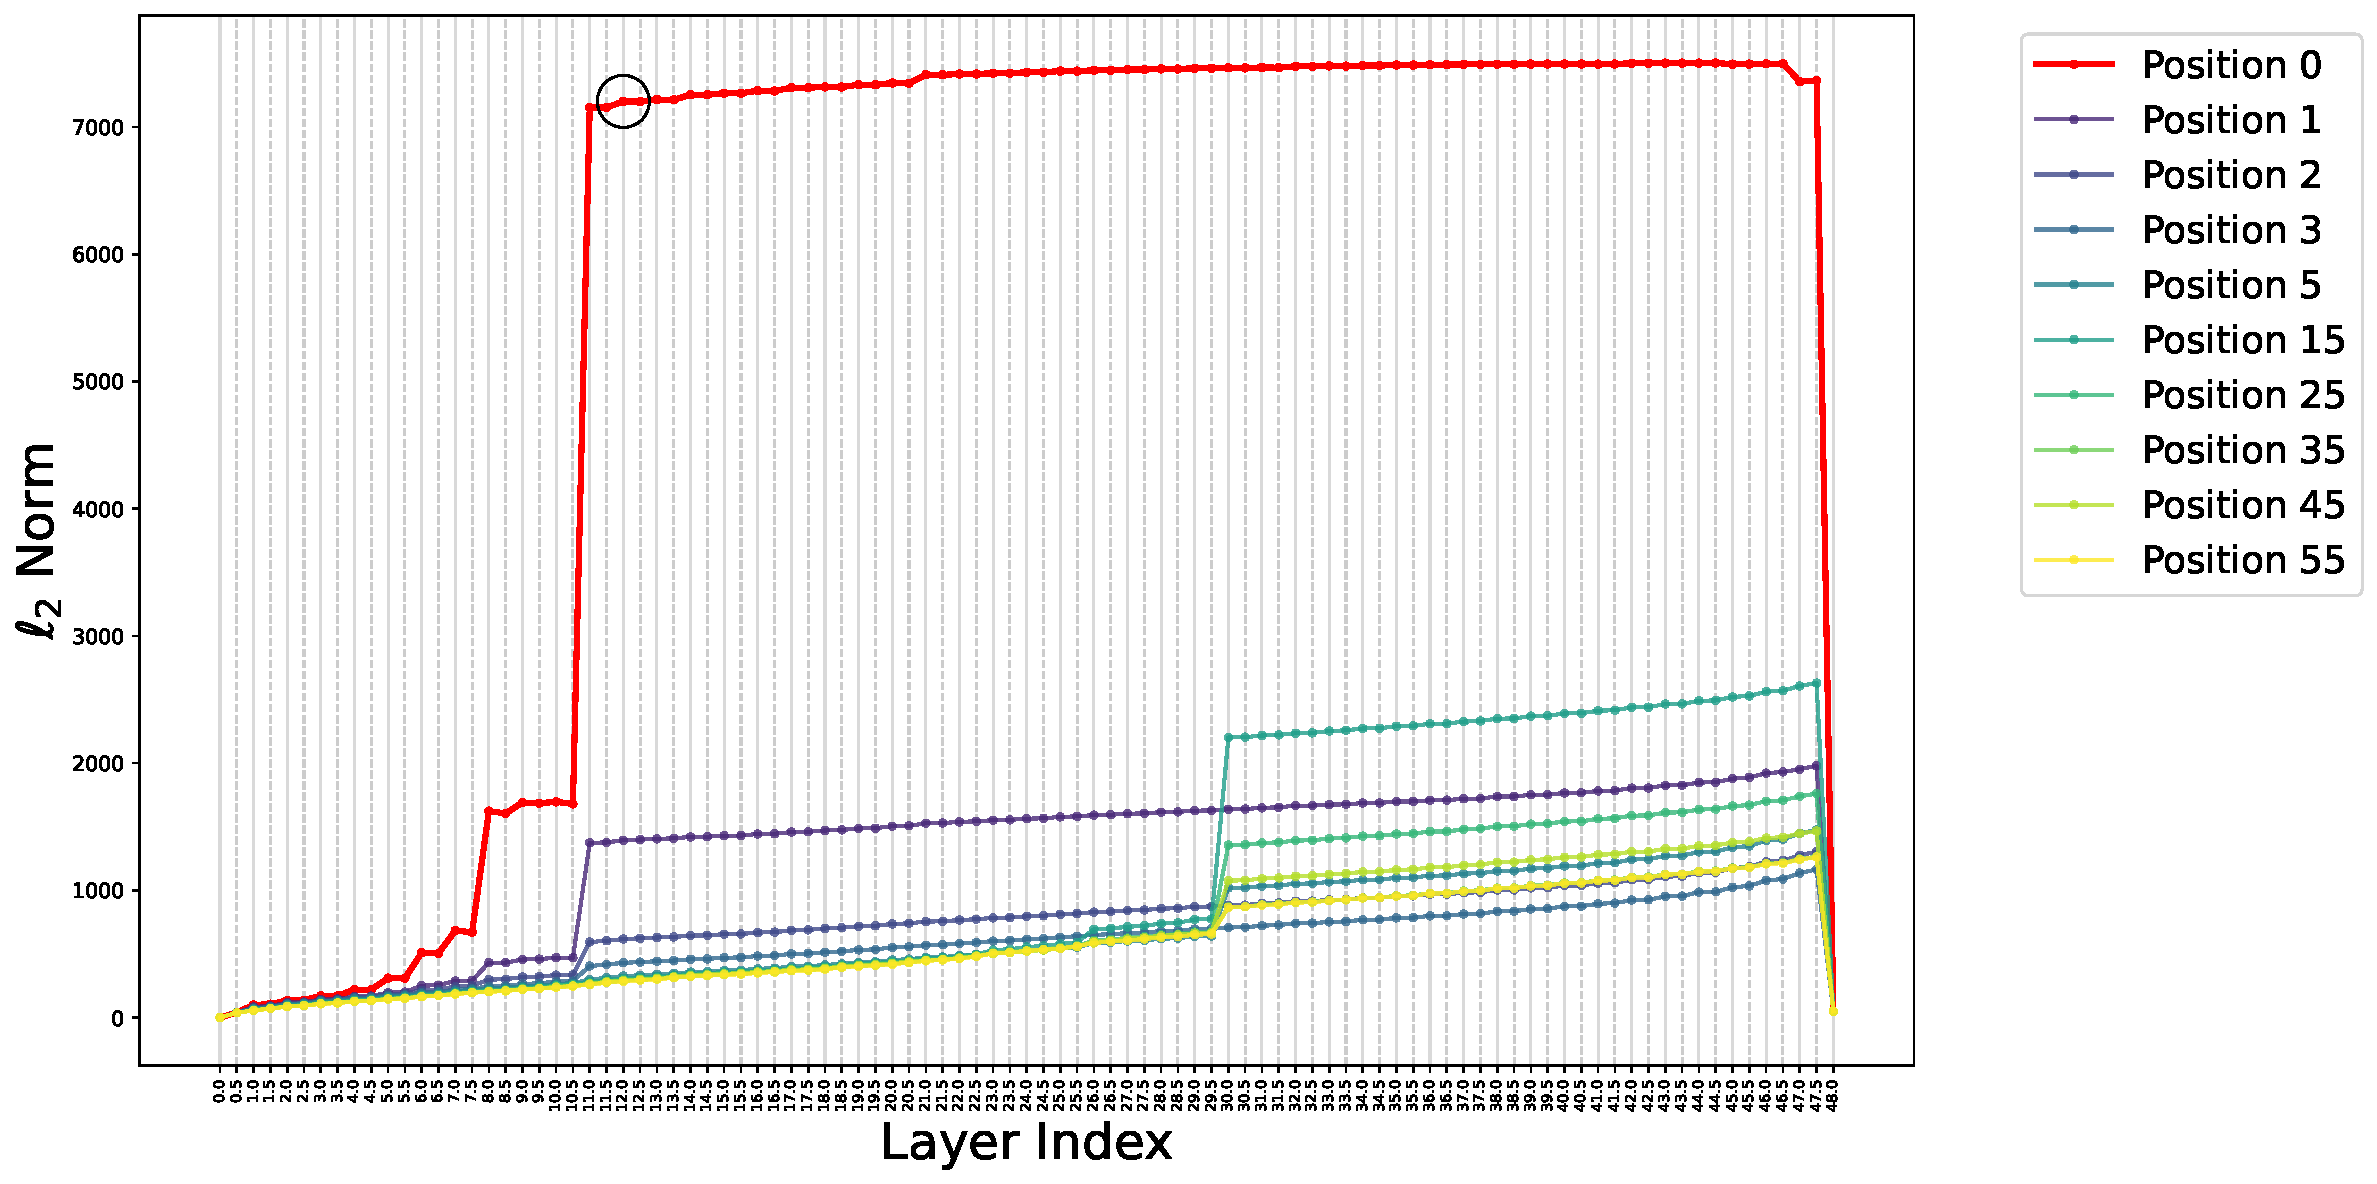
\includegraphics[width=0.95\columnwidth]{figures/fig6/fig6_step2000_l2norm.pdf}
    \end{subfigure}
    \begin{subfigure}[b]{0.95\linewidth} 
        \centering
        \caption{\scriptsize{Cosine Similarity to Position-Wise Mean}}
        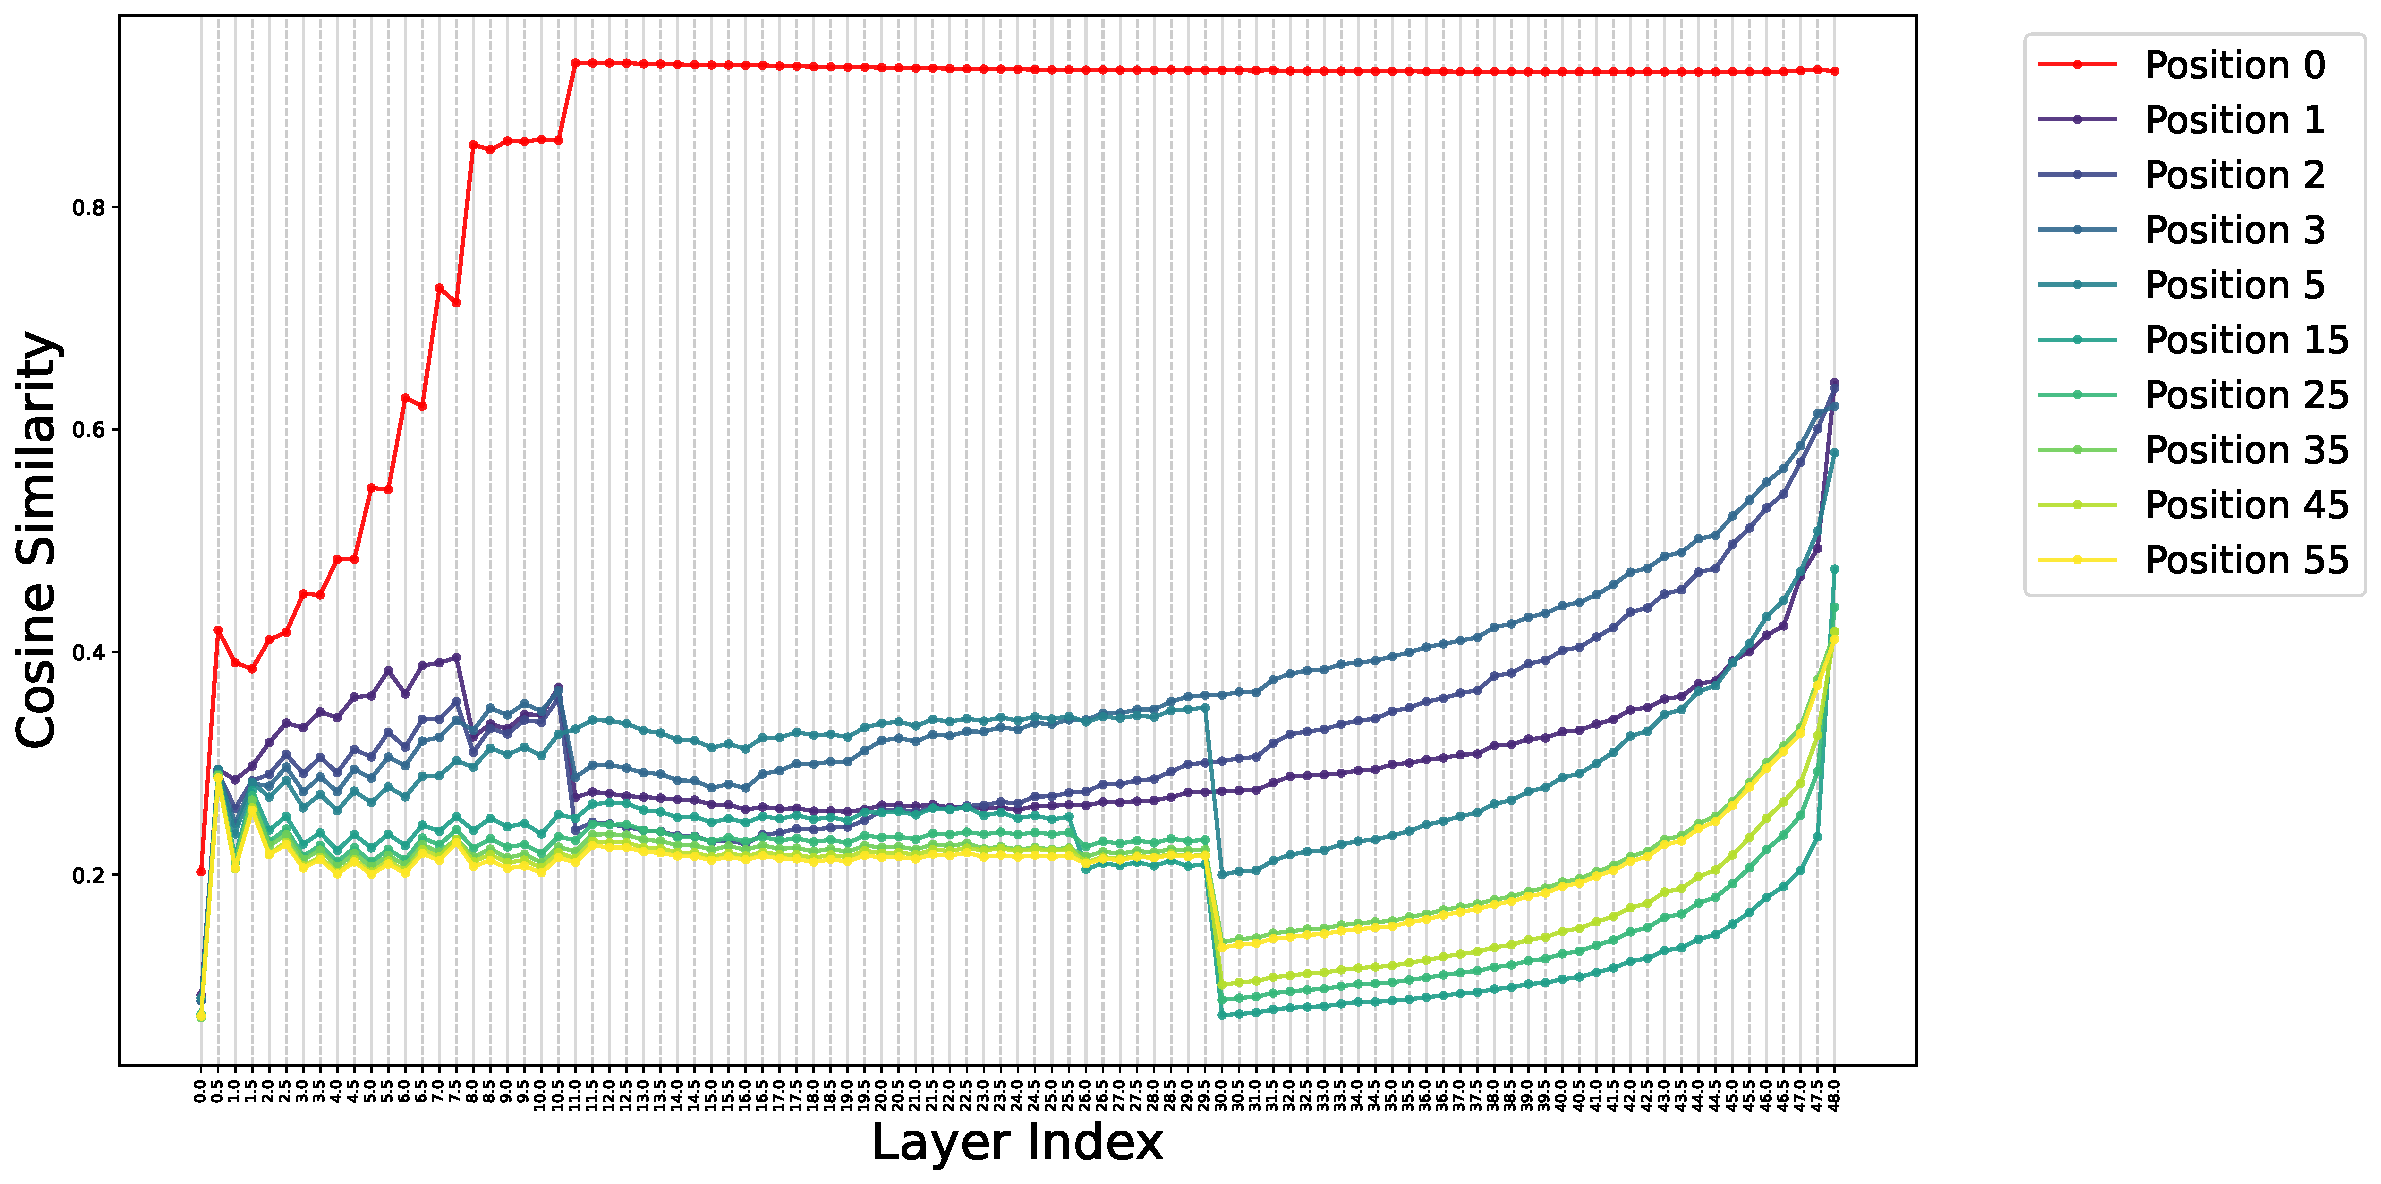
\includegraphics[width=0.95\columnwidth]{figures/fig6/fig6_step2000_sim.pdf}
    \end{subfigure}
    \begin{subfigure}[b]{0.95\linewidth} 
        \centering
        \caption{\scriptsize{Average Attention Score, Layer 12}}
        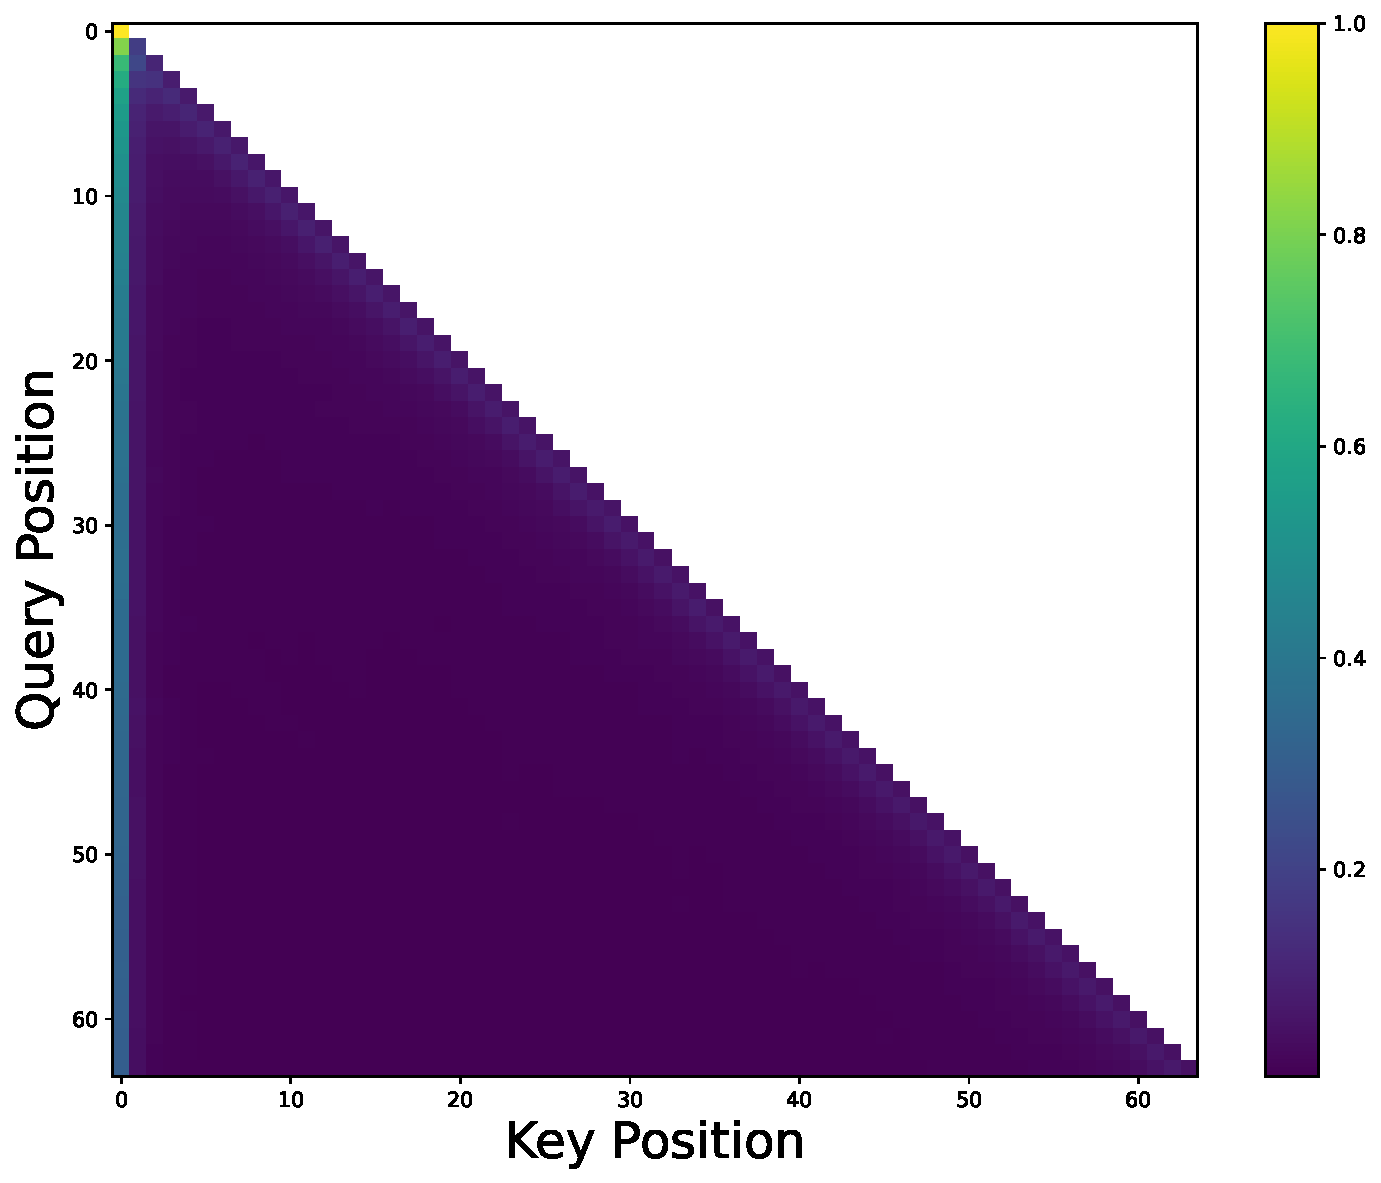
\includegraphics[width=0.7\columnwidth]{figures/fig6/fig6_step2000_layer12_attention.pdf}
    \end{subfigure}
\end{minipage}
\begin{minipage}[b]{0.32\linewidth} 
    \centering
    \begin{subfigure}[b]{0.95\linewidth} 
        \centering
        \caption{\scriptsize{Hidden States $\ell_2$Norm \\ Step 30000 ($\sim$230B Token)}}
        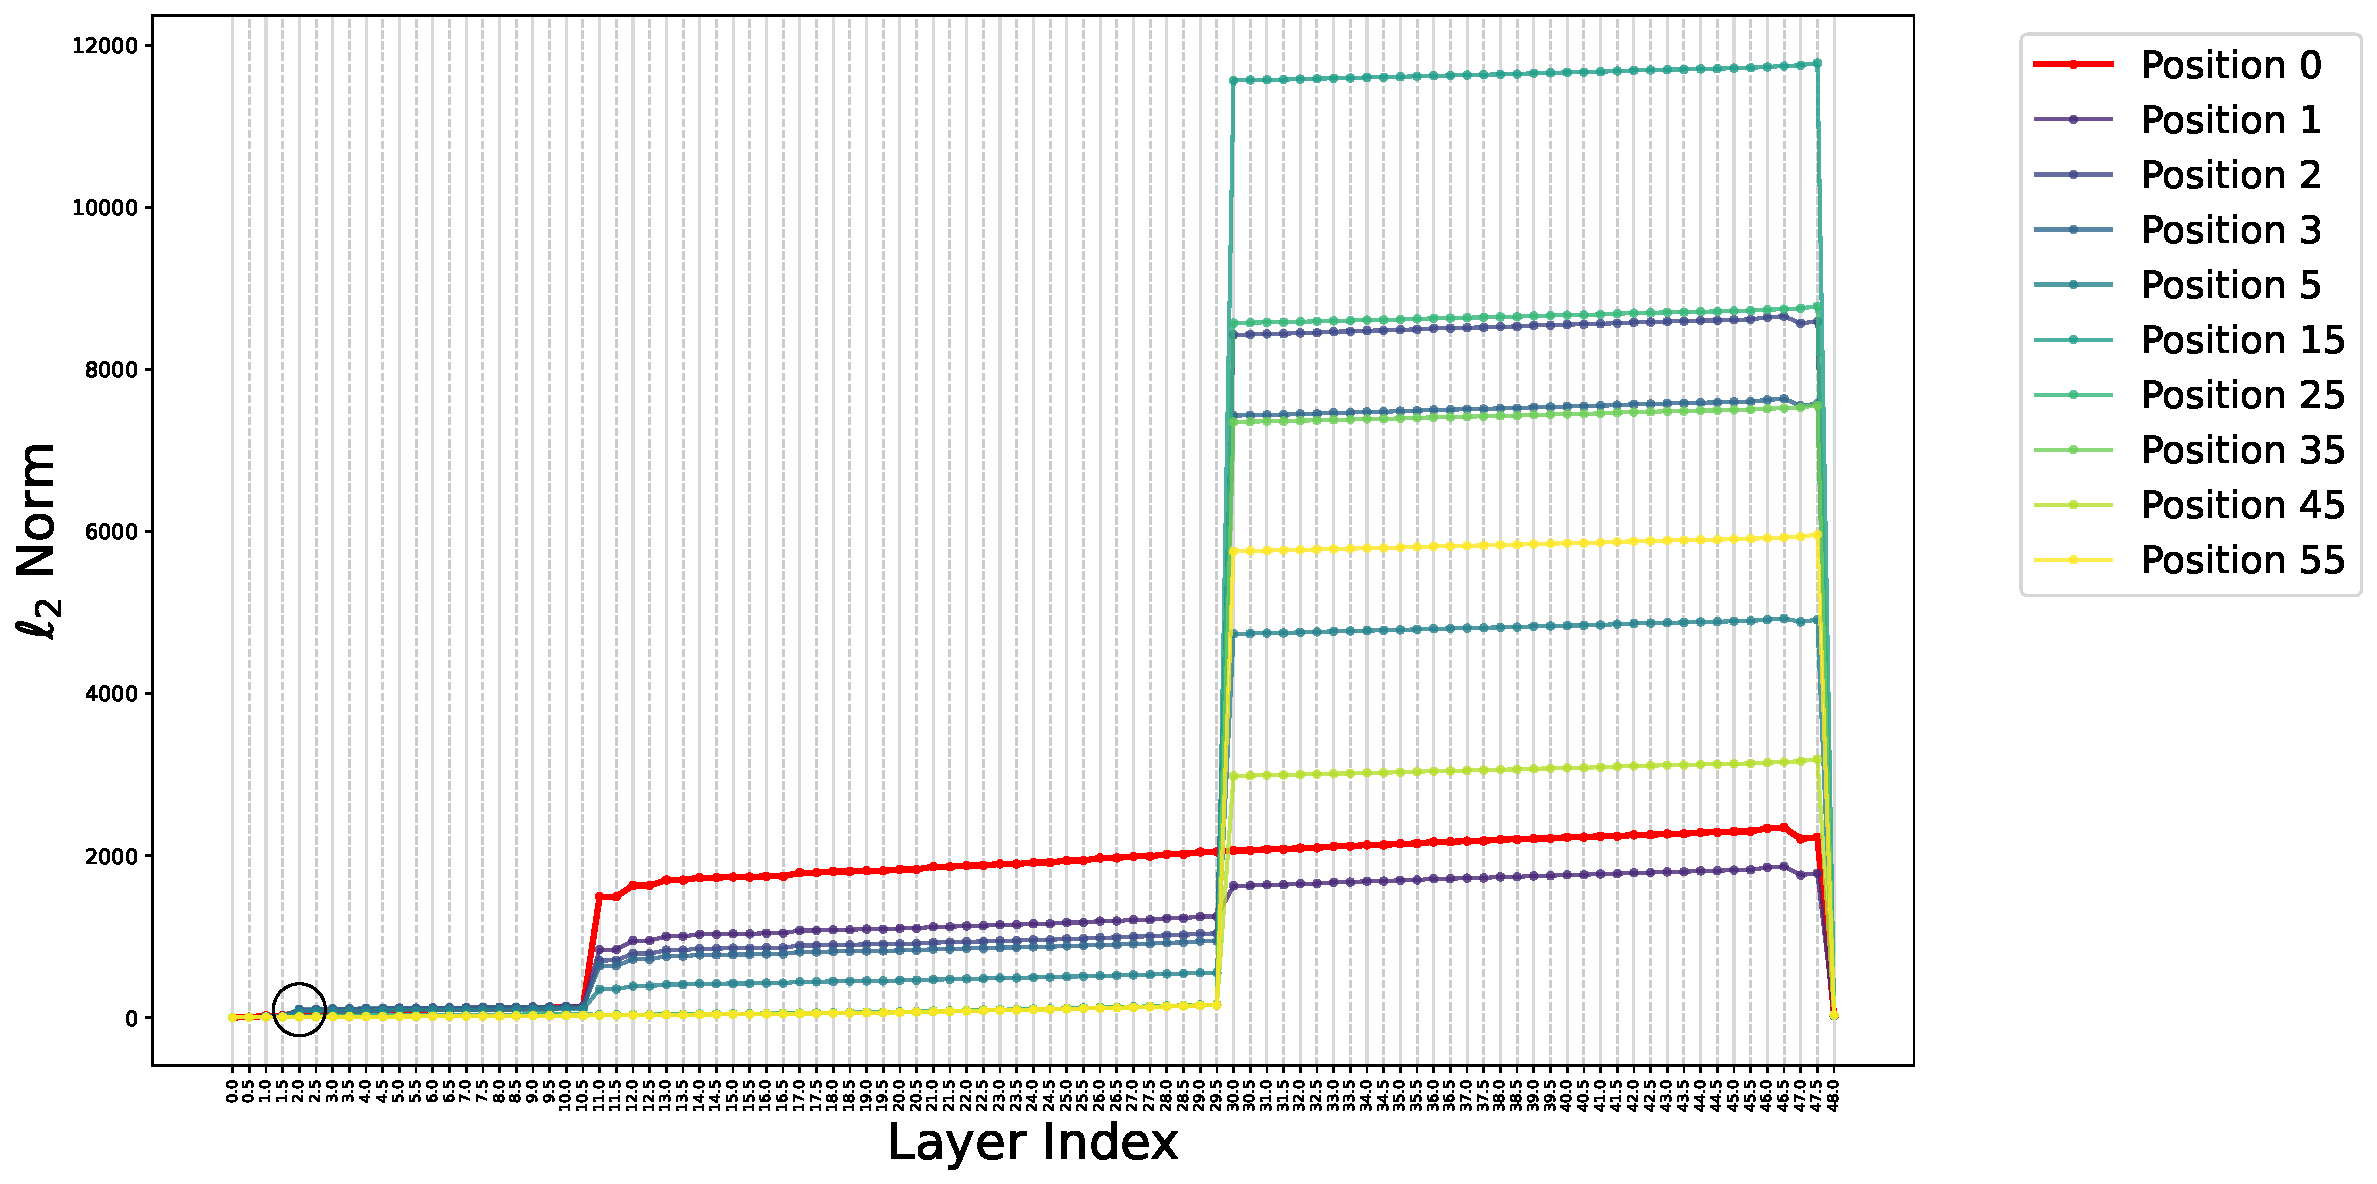
\includegraphics[width=0.95\columnwidth]{figures/fig6/fig6_step30000_l2norm.pdf}
    \end{subfigure}
    \begin{subfigure}[b]{0.95\linewidth} 
        \centering
        \caption{\scriptsize{Cosine Similarity to Position-Wise Mean}}
        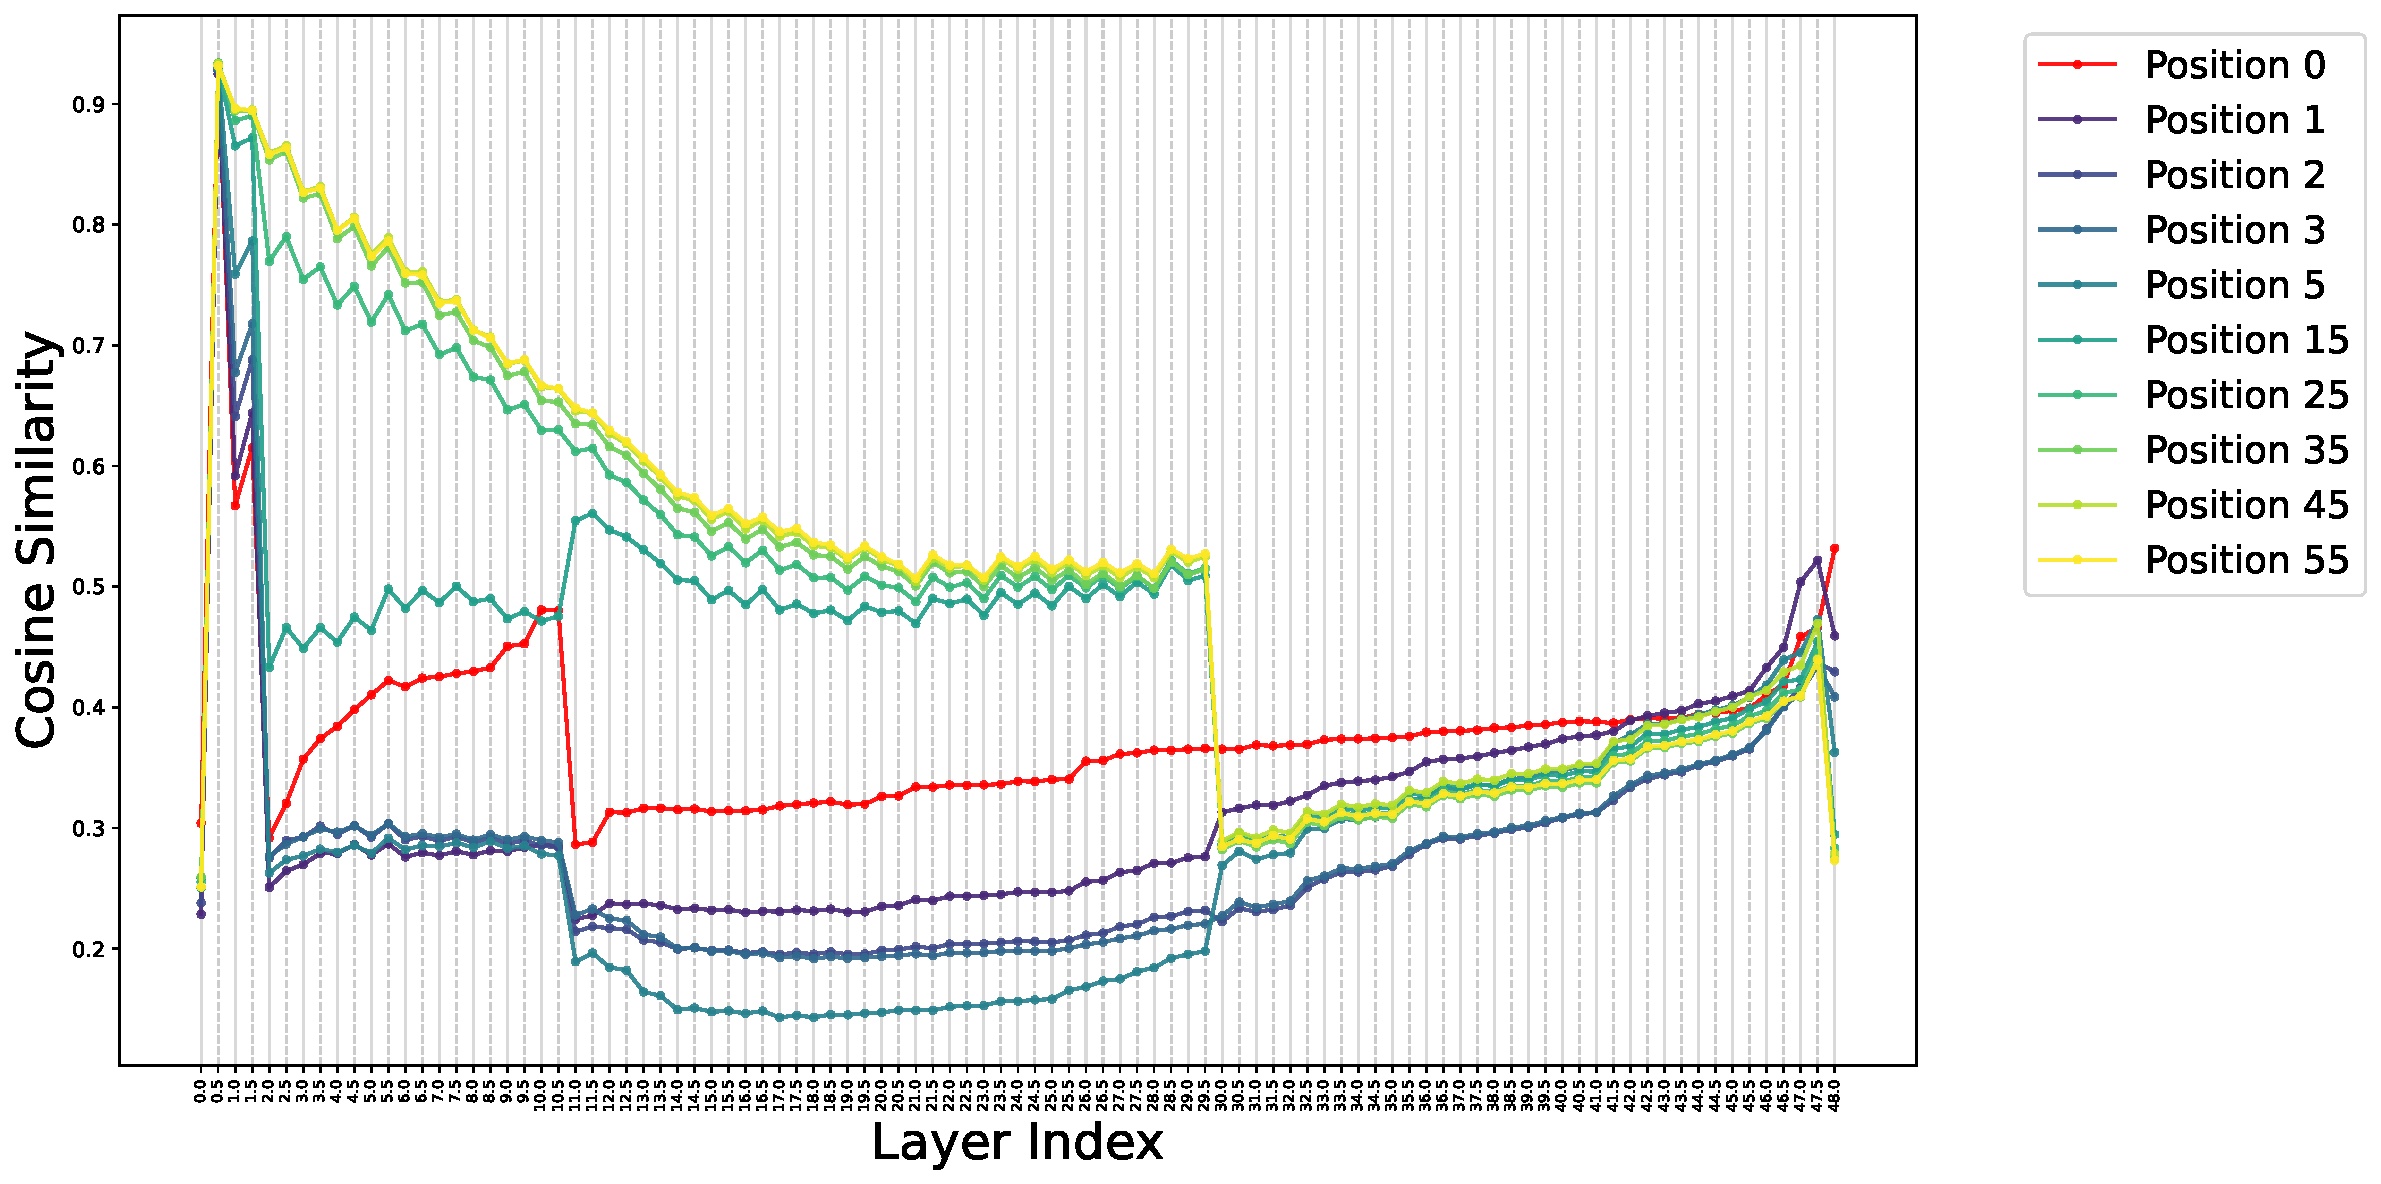
\includegraphics[width=0.95\columnwidth]{figures/fig6/fig6_step30000_sim.pdf}
    \end{subfigure}
    \begin{subfigure}[b]{0.95\linewidth} 
        \centering
        \caption{\scriptsize{Average Attention Score, Layer 2}}
        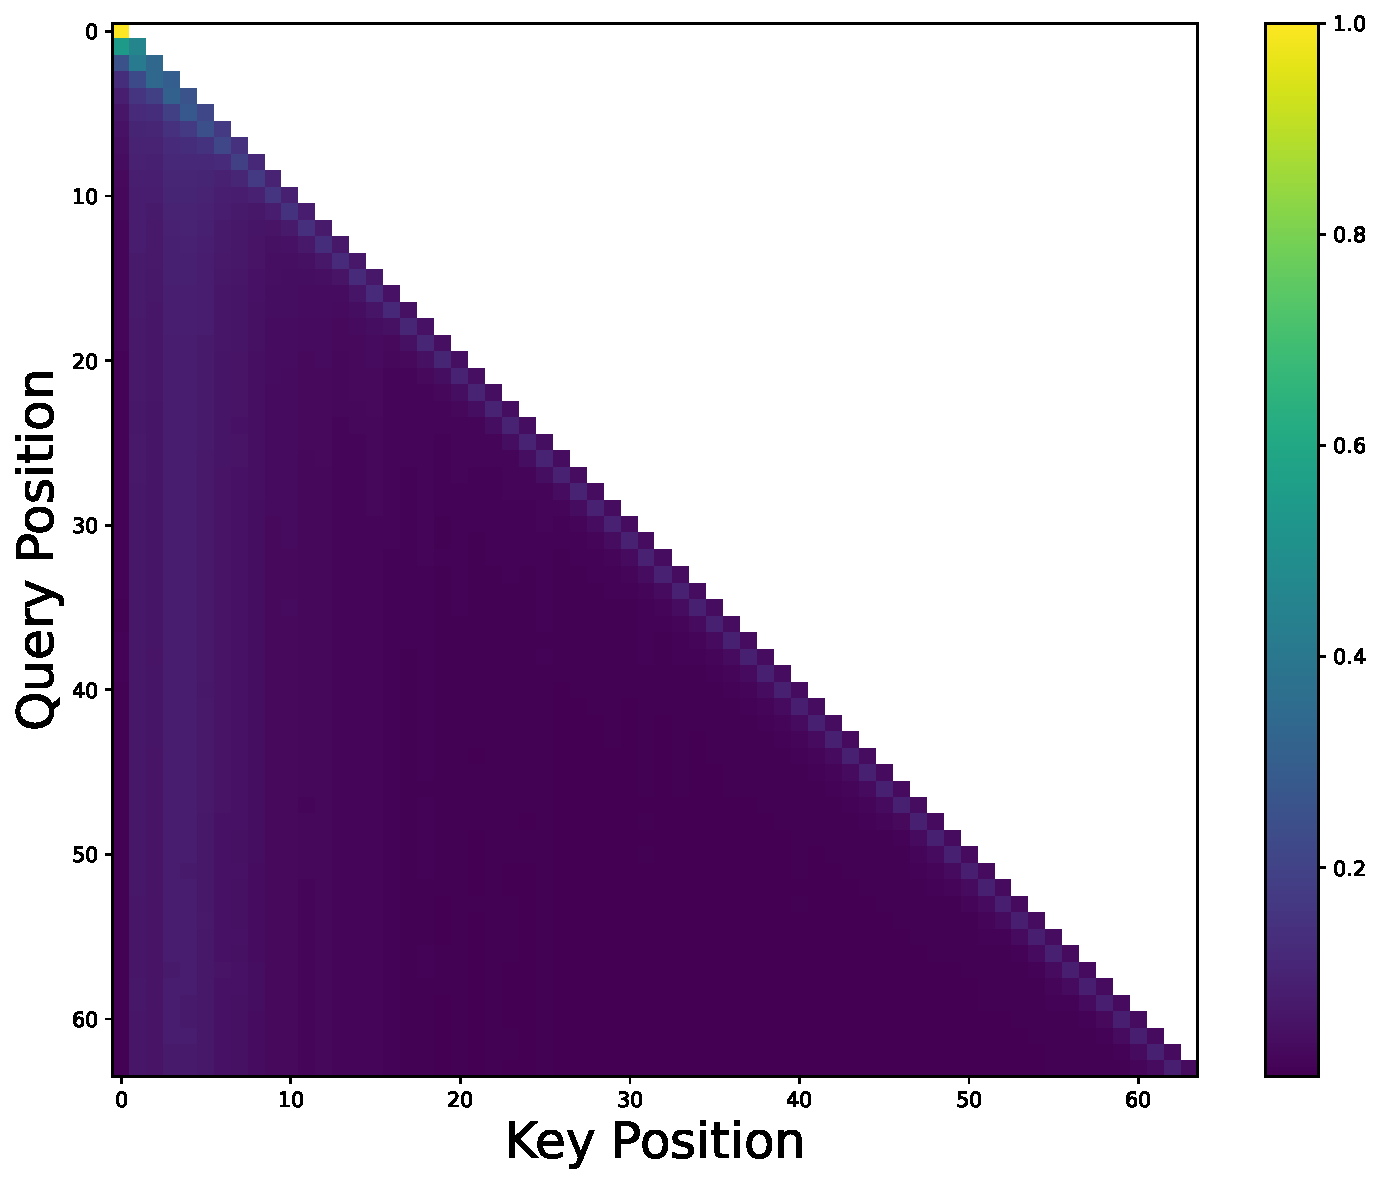
\includegraphics[width=0.7\columnwidth]{figures/fig6/fig6_step30000_layer2_attention.pdf}
    \end{subfigure}
\end{minipage}
\begin{minipage}[b]{0.32\linewidth} 
    \centering
    \begin{subfigure}[b]{0.95\linewidth} 
        \centering
        \caption{\scriptsize{Hidden States $\ell_2$Norm \\ Step 60000 ($\sim$460B Token)}}
        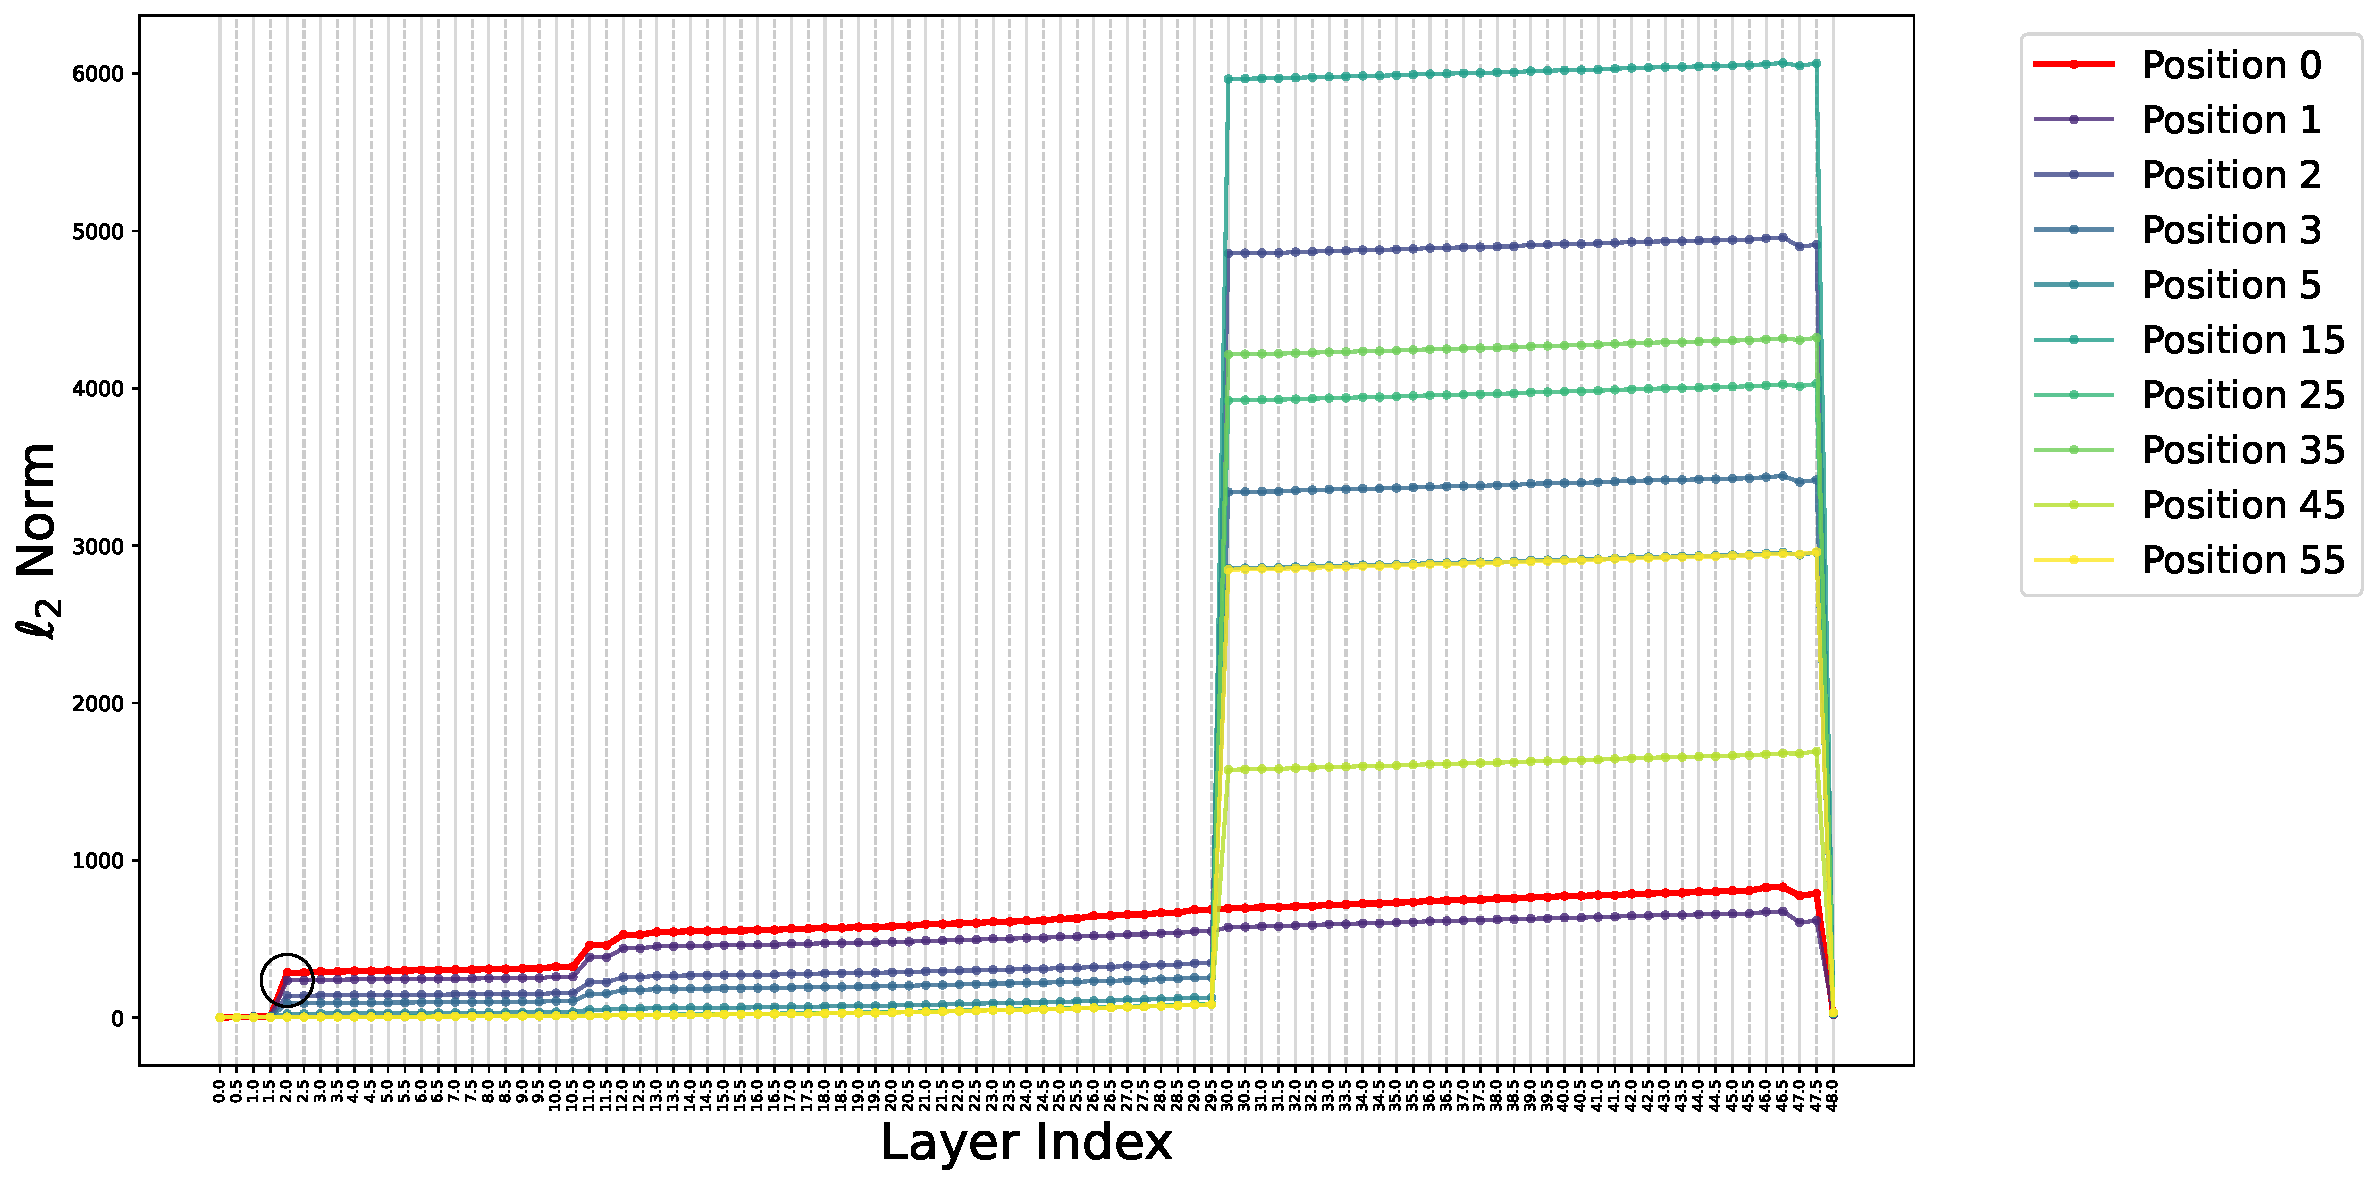
\includegraphics[width=0.95\columnwidth]{figures/fig6/fig6_step60000_l2norm.pdf}
    \end{subfigure}
    \begin{subfigure}[b]{0.95\linewidth} 
        \centering
        \caption{\scriptsize{Cosine Similarity to Position-Wise Mean}}
        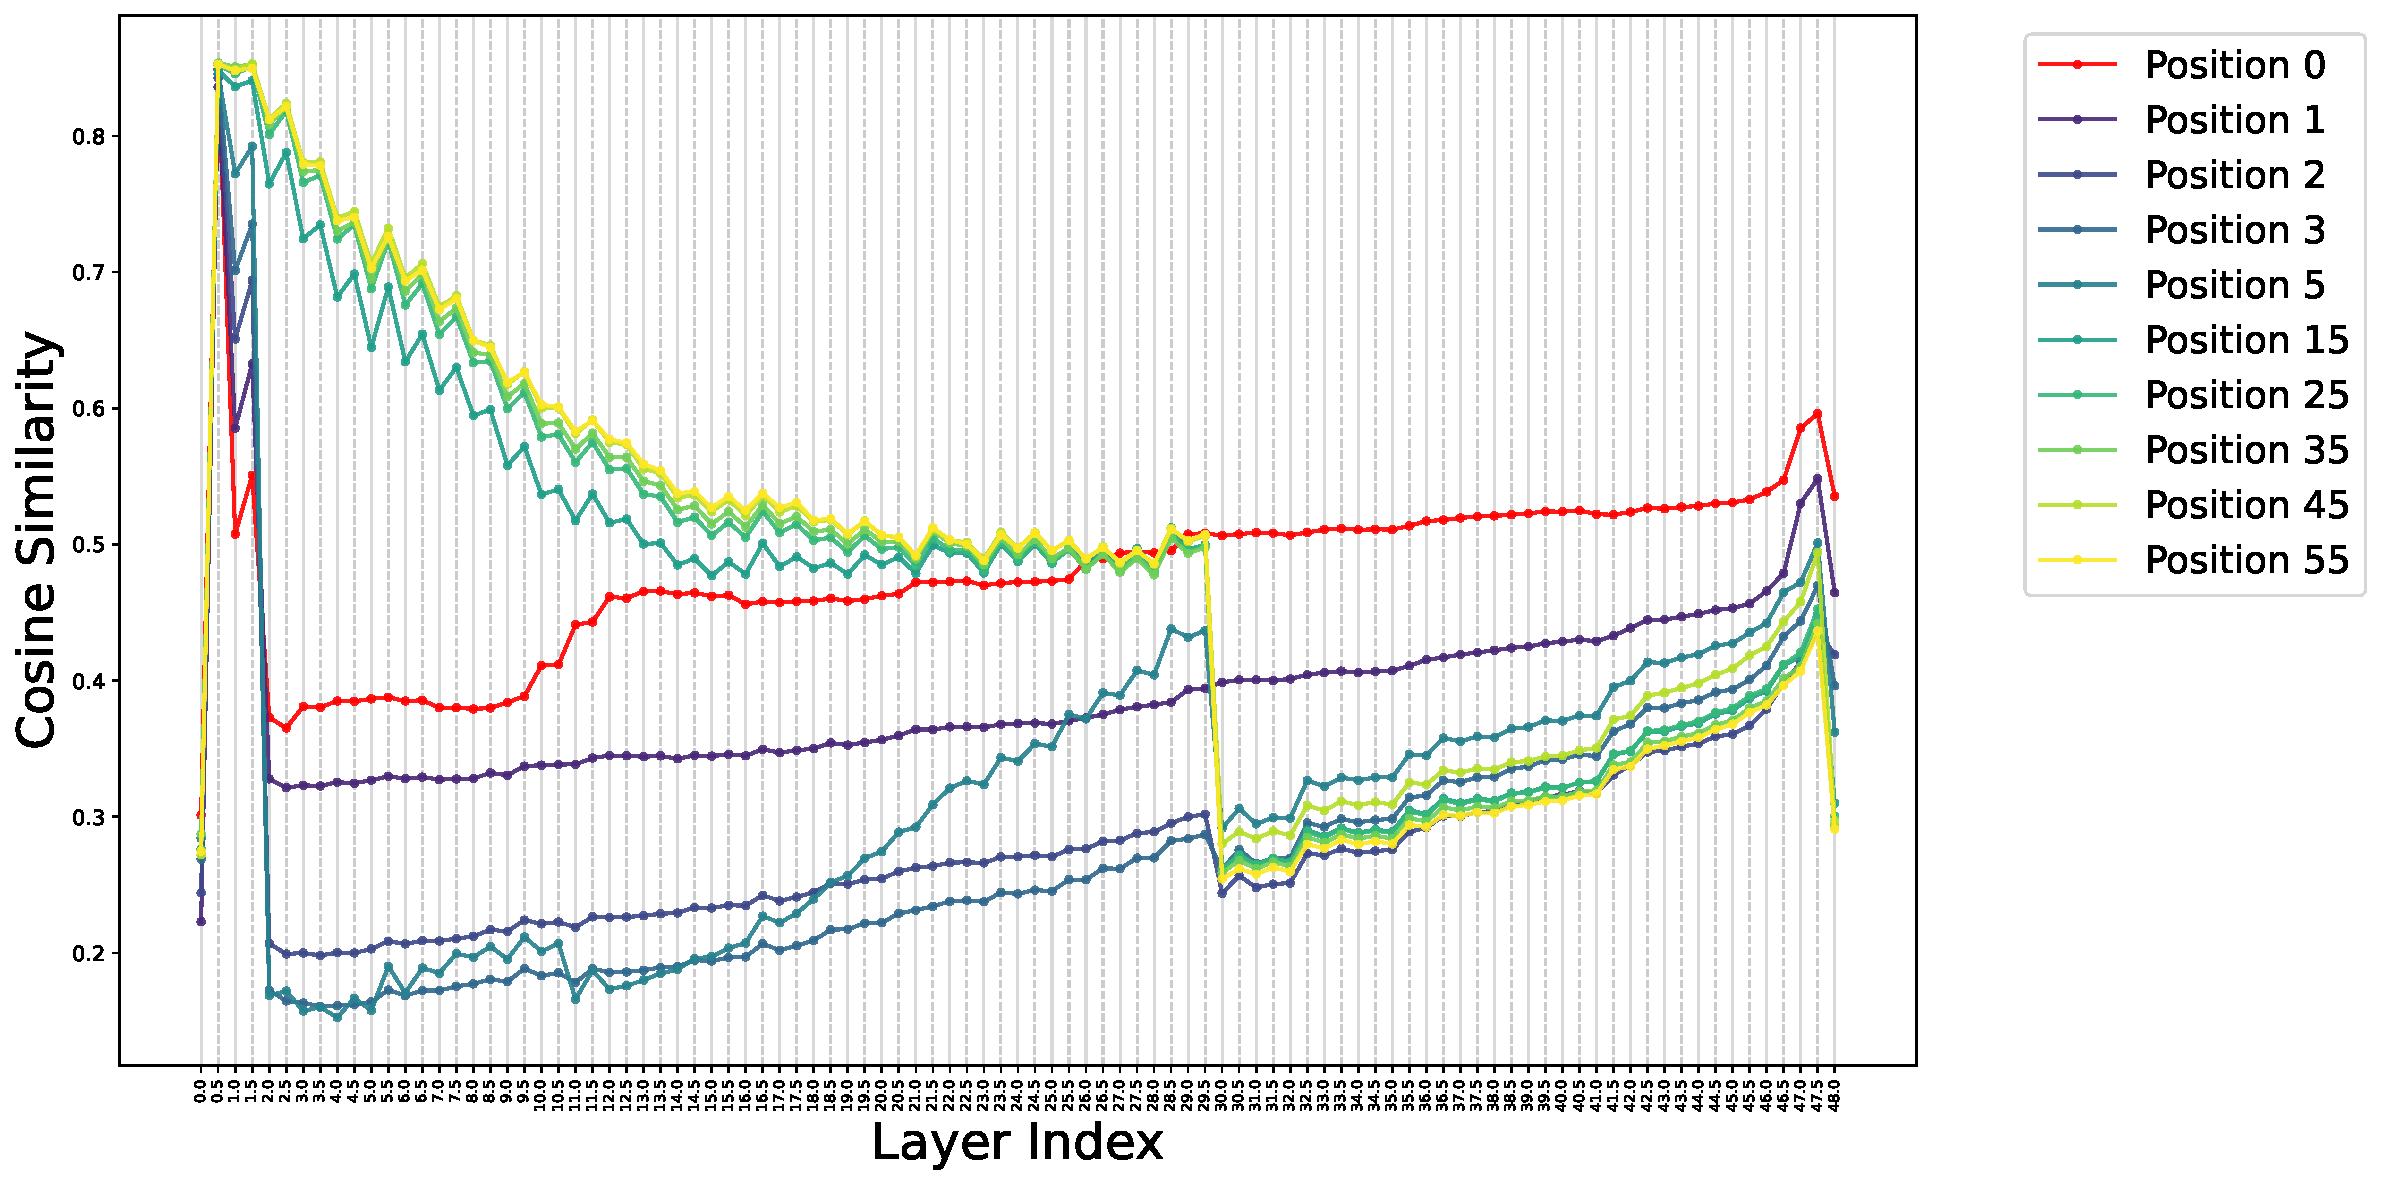
\includegraphics[width=0.95\columnwidth]{figures/fig6/fig6_step60000_sim.pdf}
    \end{subfigure}
    \begin{subfigure}[b]{0.95\linewidth} 
        \centering
        \caption{\scriptsize{Average Attention Score, Layer 2}}
        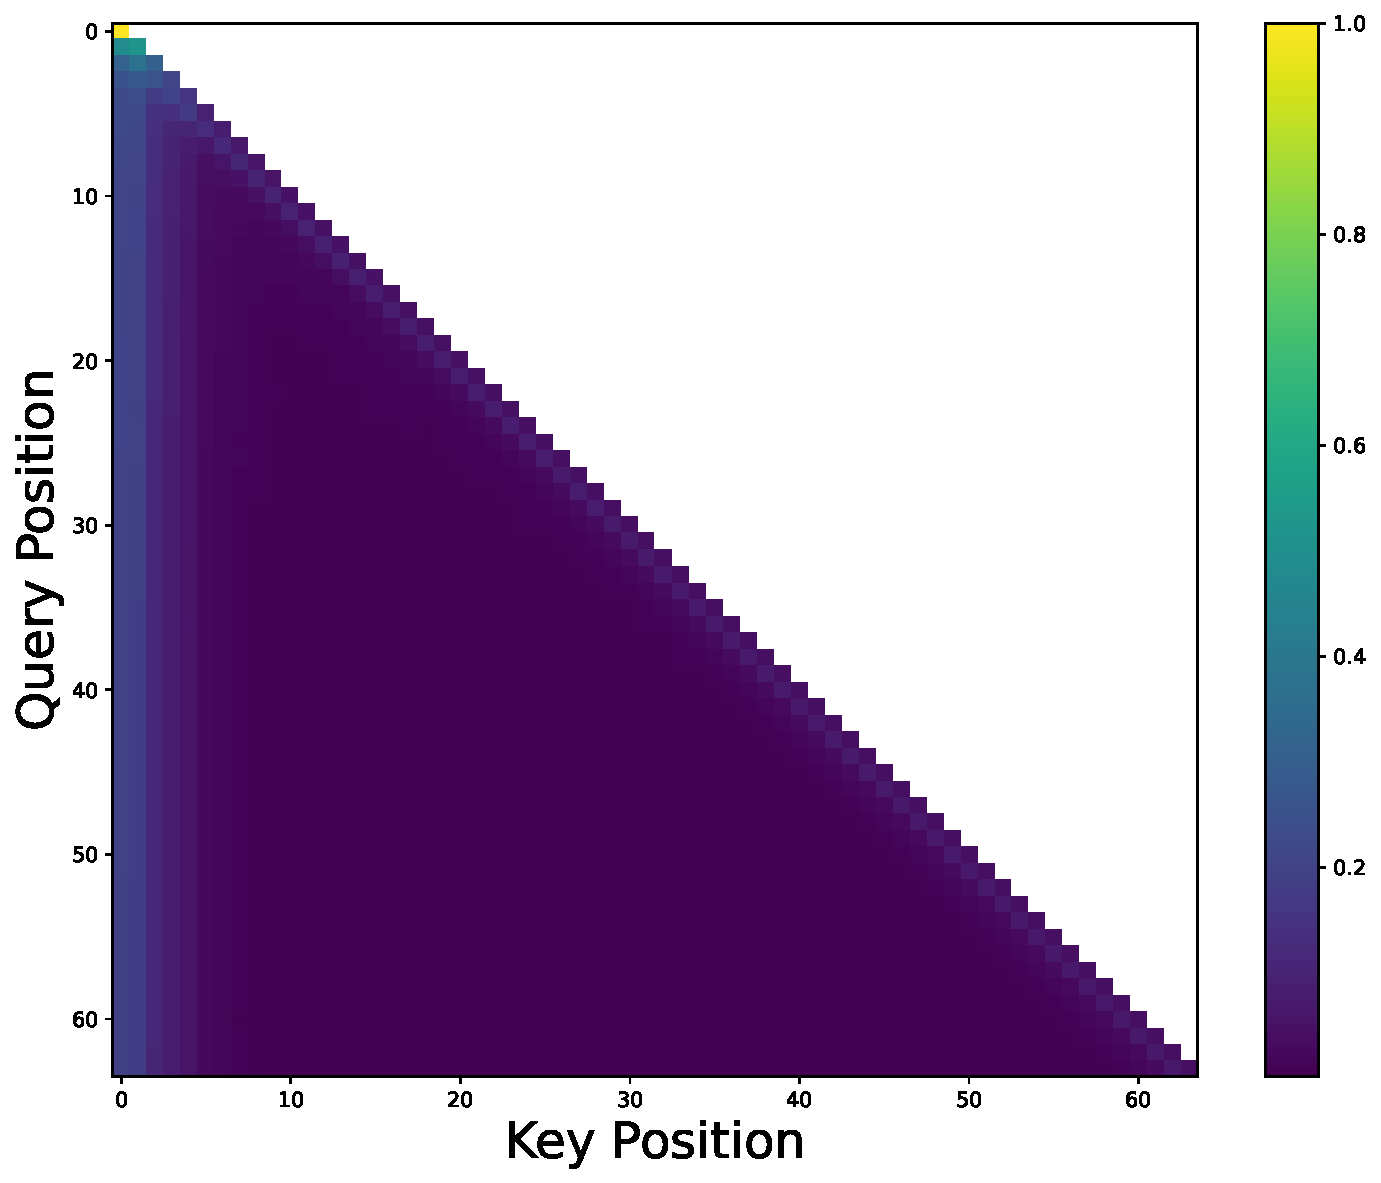
\includegraphics[width=0.7\columnwidth]{figures/fig6/fig6_step60000_layer2_attention.pdf}
    \end{subfigure}
\end{minipage}
\centering
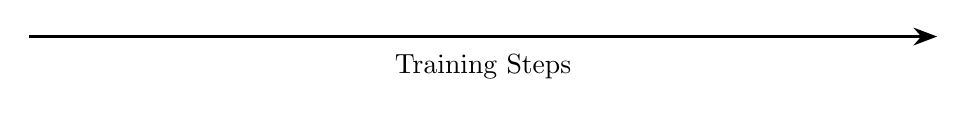
\begin{tikzpicture}
  \node[inner sep=0, minimum width=0.95\linewidth, minimum height=0pt] (box) {};
  \draw[-{Stealth[length=3mm]}, line width=0.98pt]
    (box.west) -- (box.east) node[midway, below=1mm] {Training Steps};
\end{tikzpicture}
\vspace{-1em}
\caption{Early-stage training statistics showing a rise in P0 $\ell_2$ norms and sink emergence in middle layers. As training continues, these fade into broader multi-position sinks. \textbf{Position-wise Mean} is computed across samples per position and layer.}
\vspace{-1em}
\label{fig-early-stage}
\end{figure*}

\begin{figure*}[t]
    
\begin{minipage}[b]{0.32\linewidth} 
    \centering
    \begin{subfigure}[b]{0.95\linewidth} 
        \centering
        \caption{\scriptsize{Hidden States $\ell_2$Norm \\ Step 70000 ($\sim$540B Token})}
        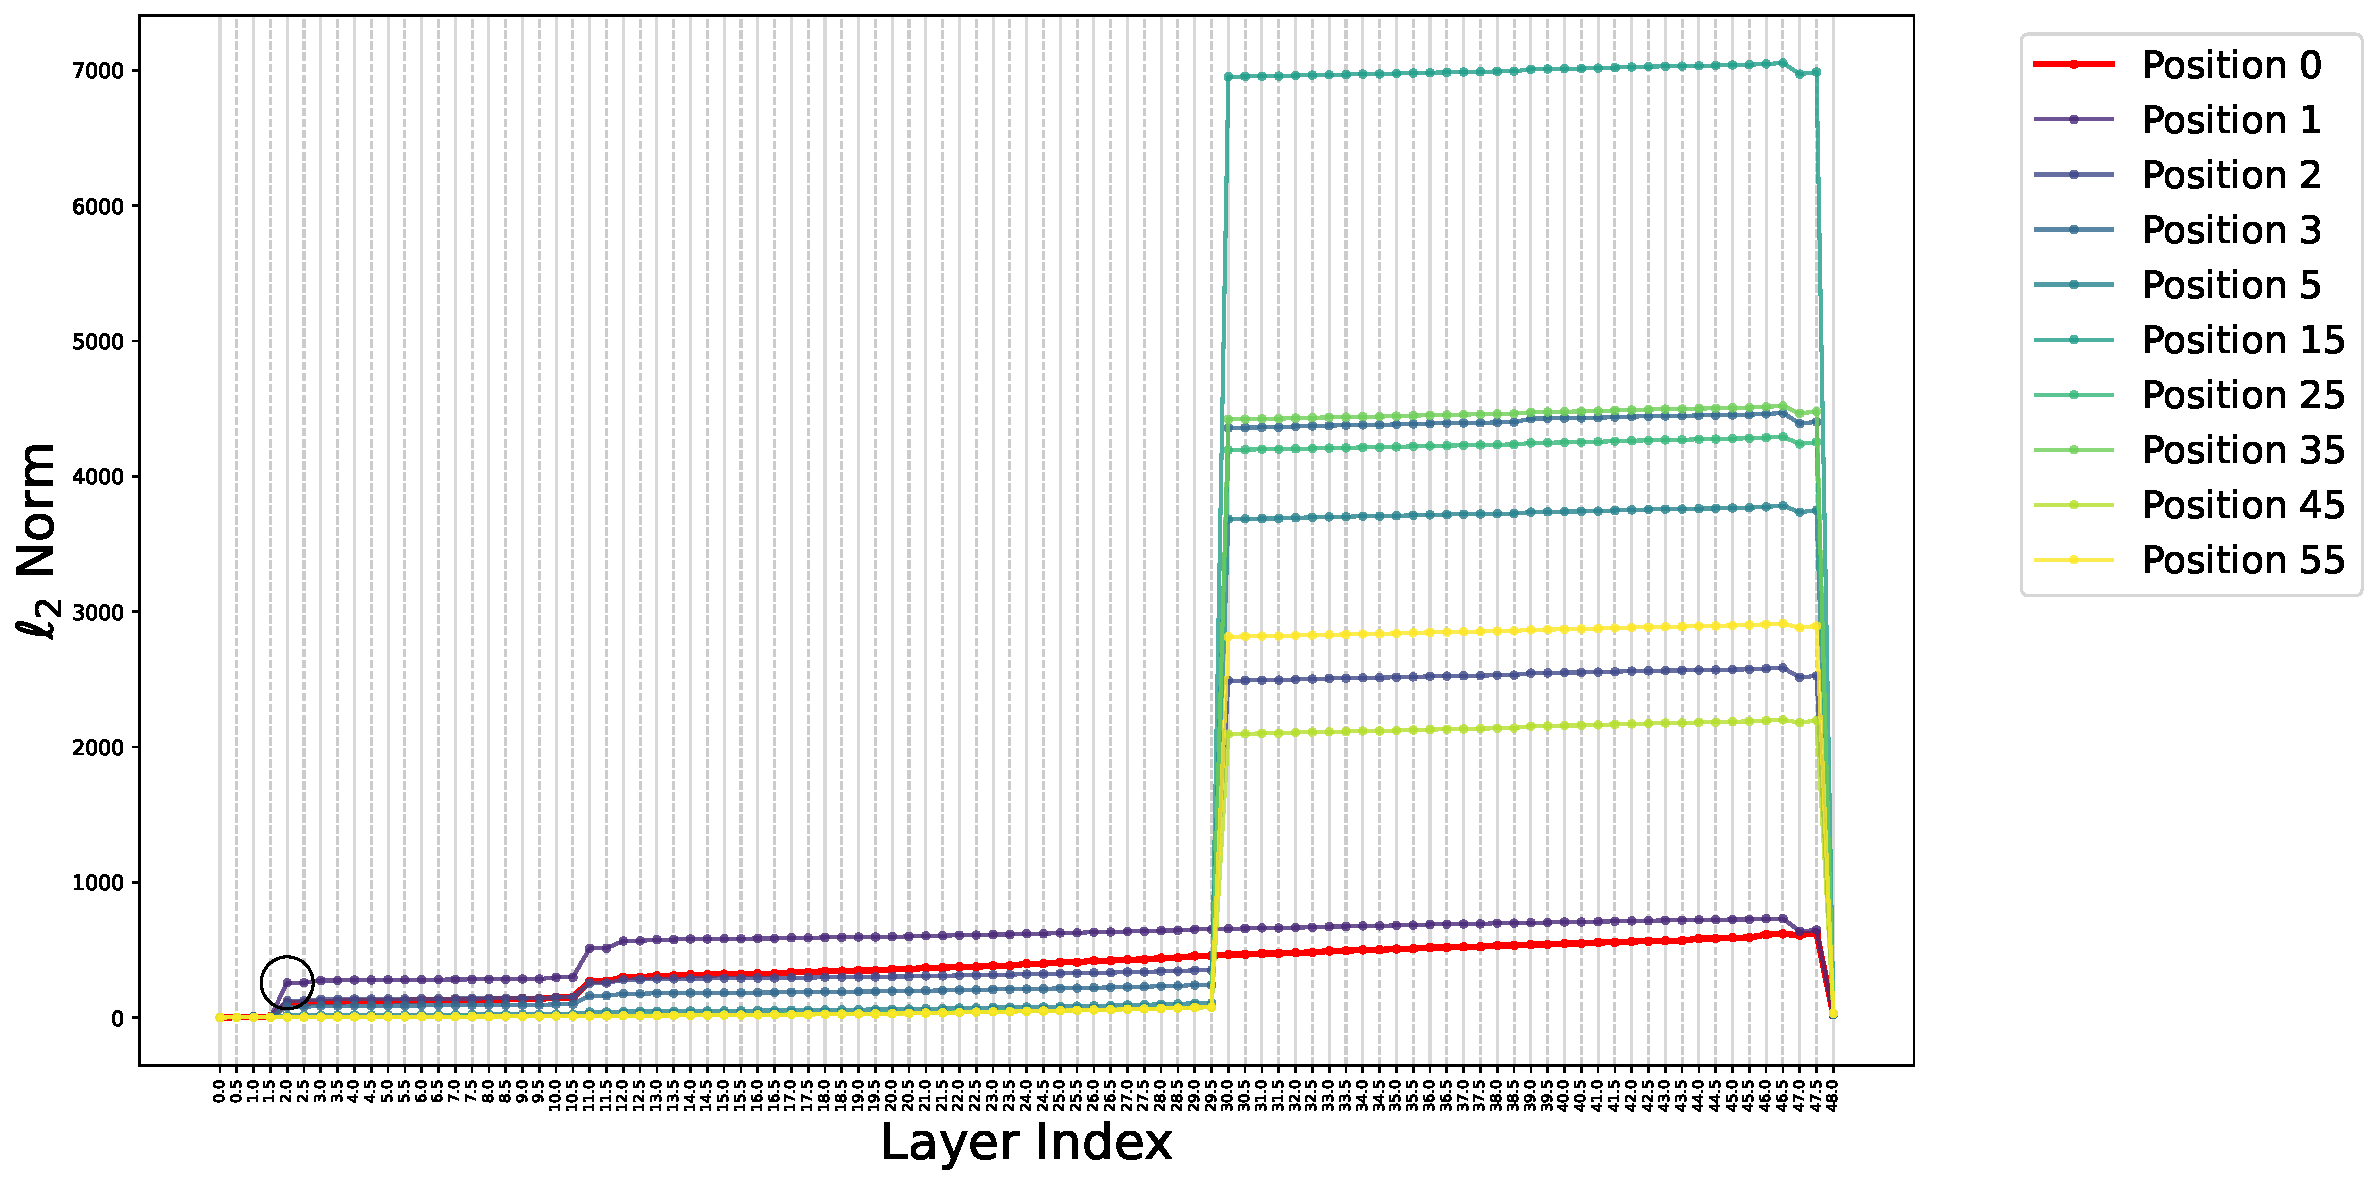
\includegraphics[width=0.95\columnwidth]{figures/fig6/fig6_step70000_l2norm.pdf}
    \end{subfigure}
    \begin{subfigure}[b]{0.95\linewidth} 
        \centering
        \caption{\scriptsize{Cosine Similarity to Position-Wise Mean}}
        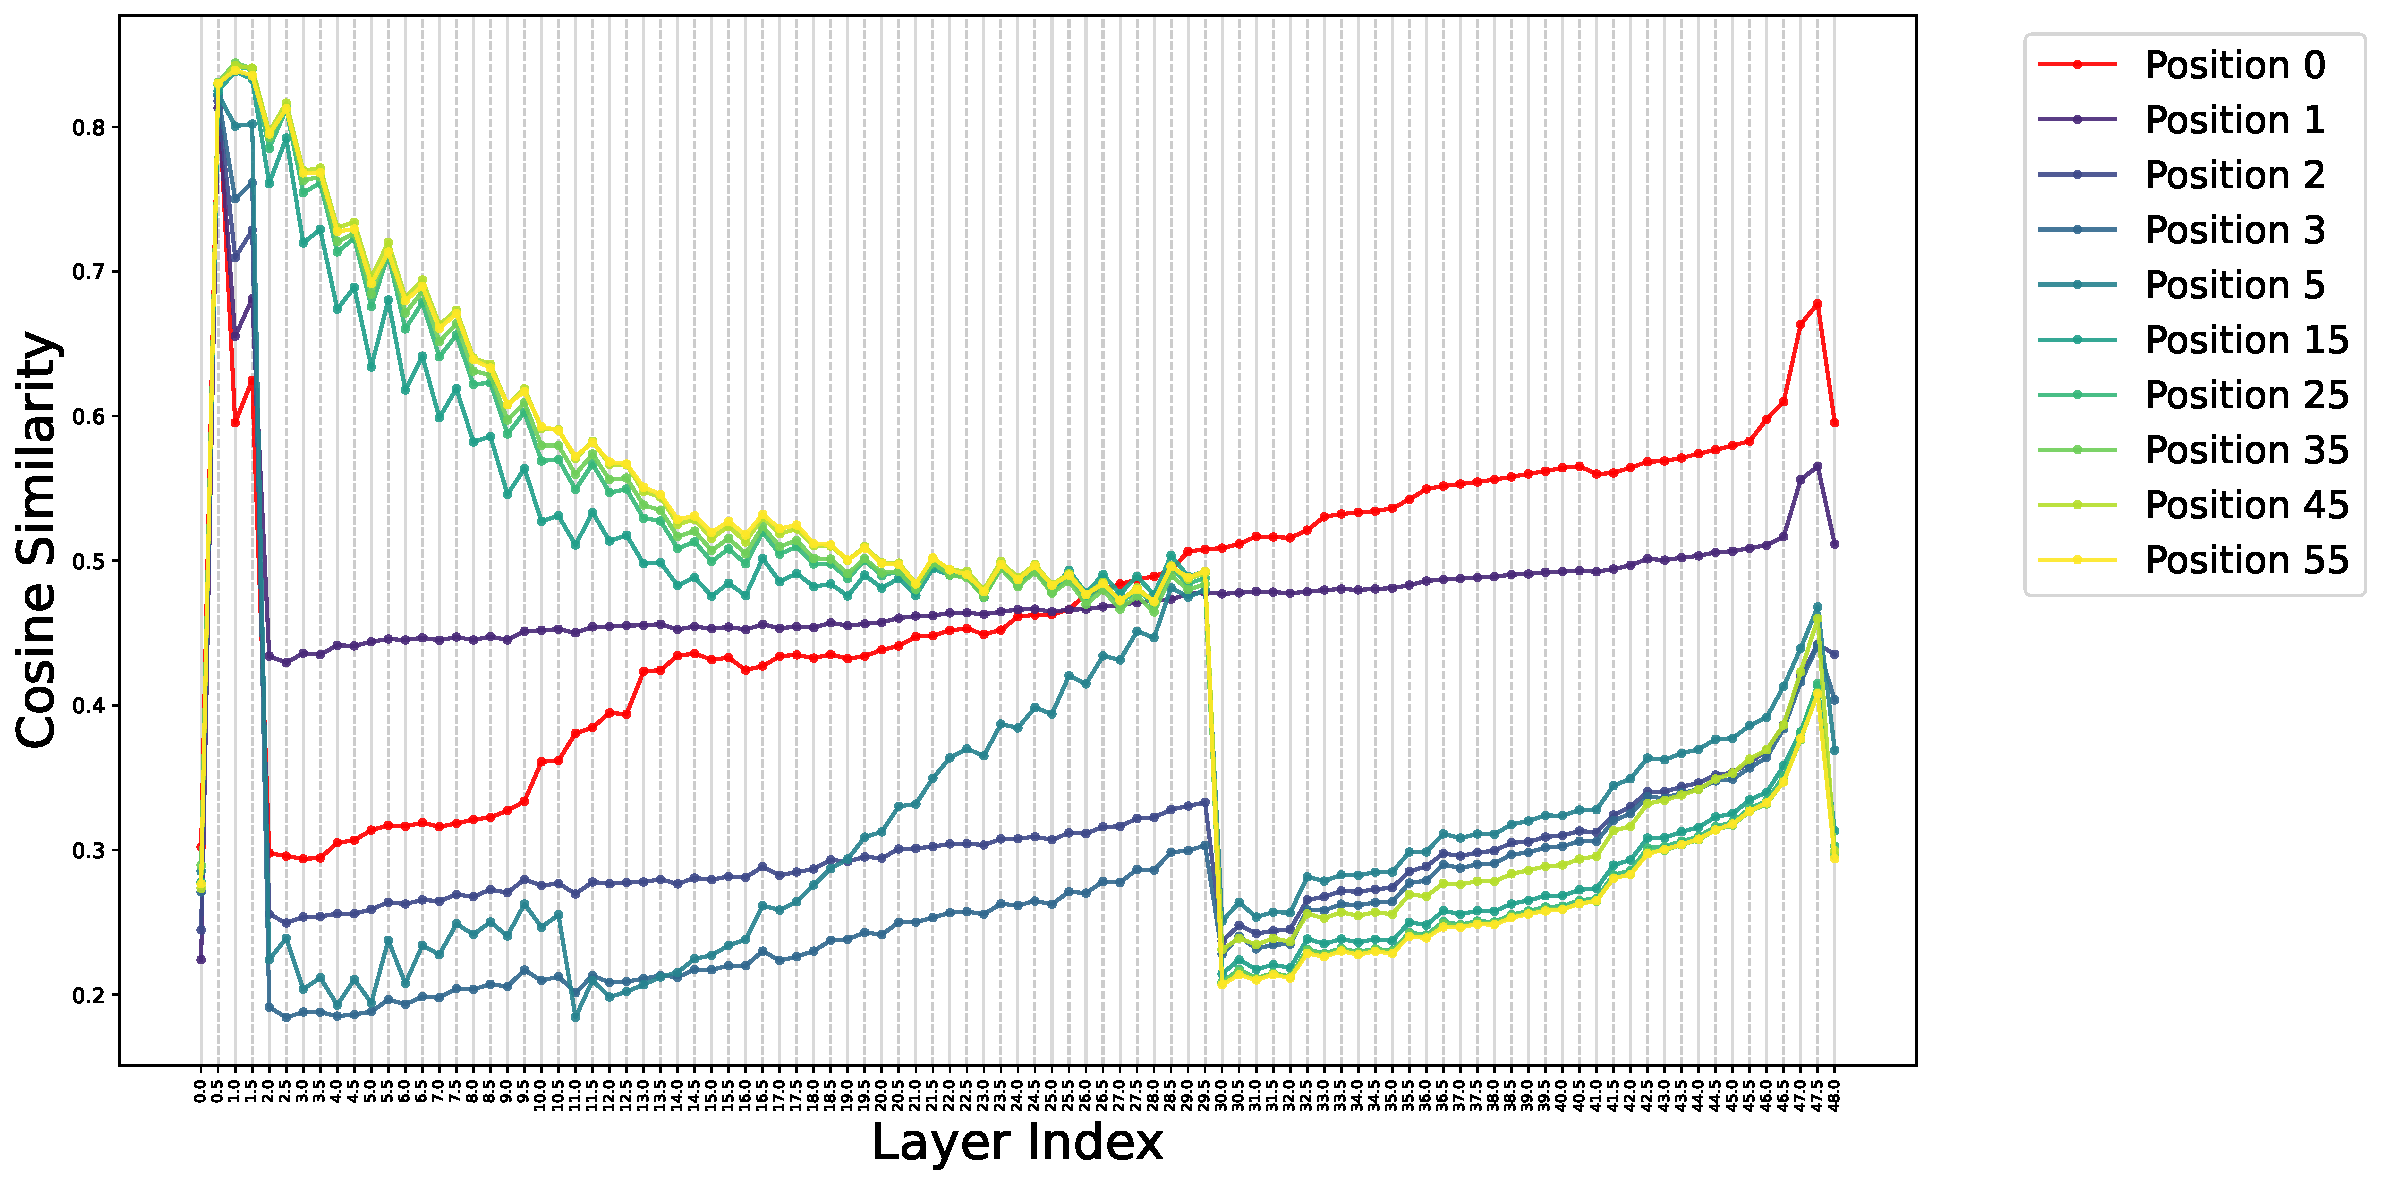
\includegraphics[width=0.95\columnwidth]{figures/fig6/fig6_step70000_sim.pdf}
    \end{subfigure}
    \begin{subfigure}[b]{0.95\linewidth} 
        \centering
        \caption{\scriptsize{Average Attention Score, Layer 2}}
        \label{fig7c}
        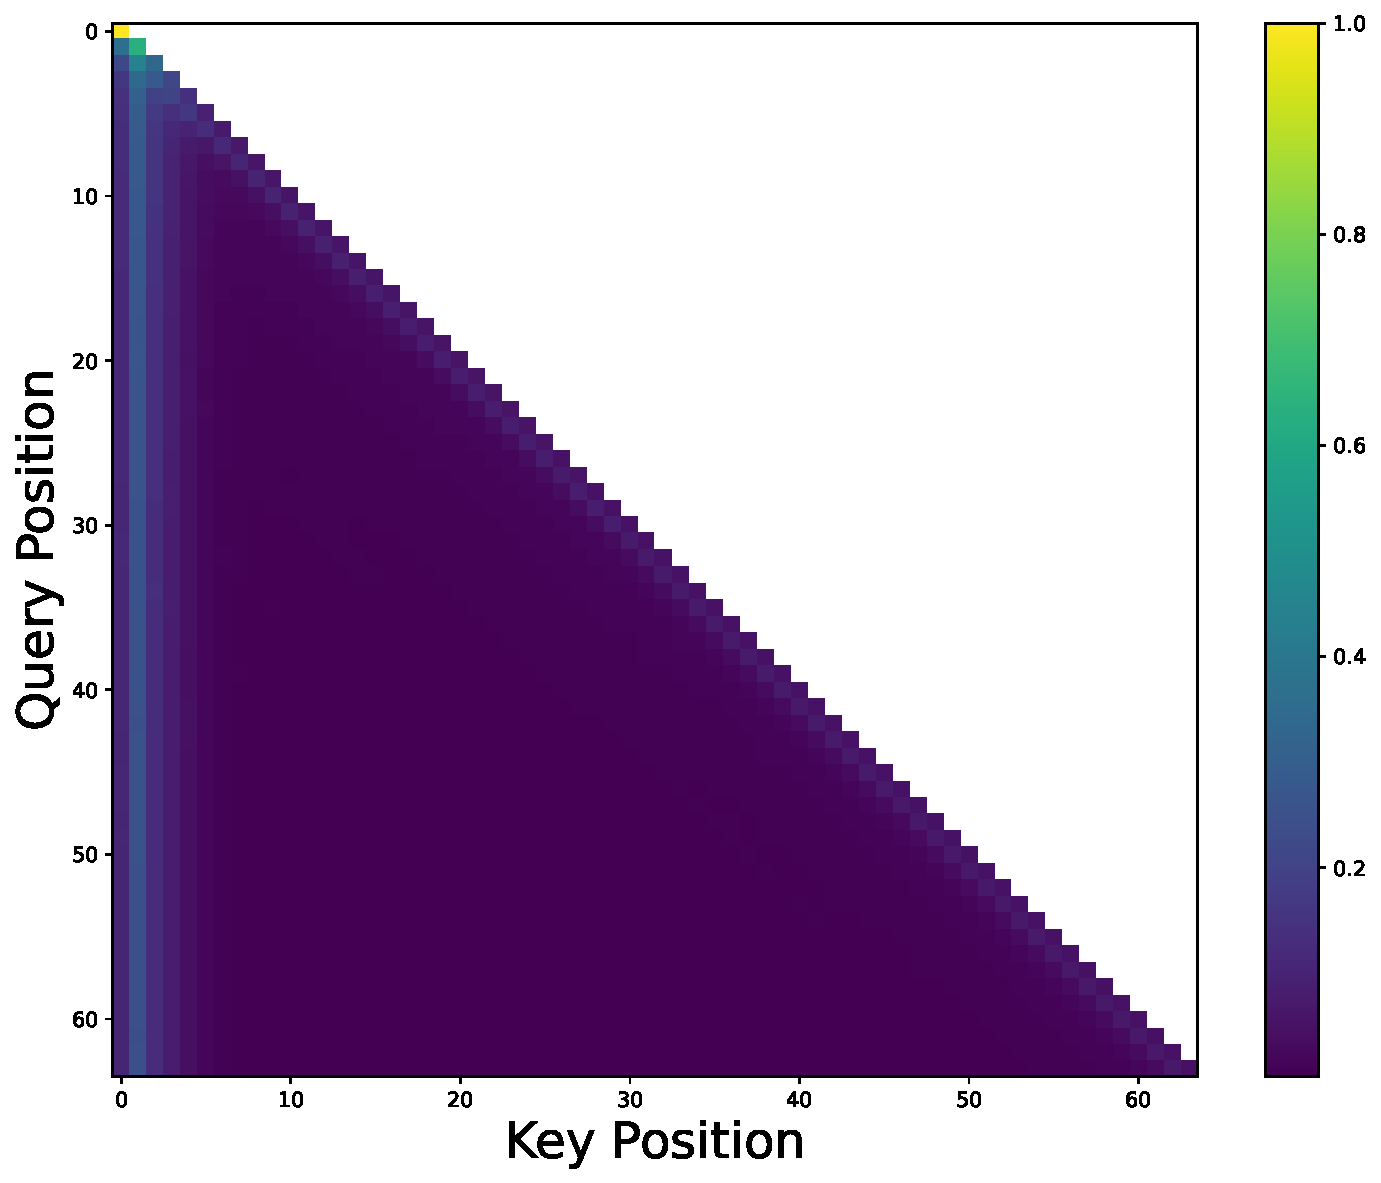
\includegraphics[width=0.7\columnwidth]{figures/fig6/fig6_step70000_layer2_attention.pdf}
    \end{subfigure}
\end{minipage}
\begin{minipage}[b]{0.32\linewidth} 
    \centering
    \begin{subfigure}[b]{0.95\linewidth} 
        \centering
        \caption{\scriptsize{Hidden States $\ell_2$Norm \\ Step 80000 ($\sim$620B Token})}
        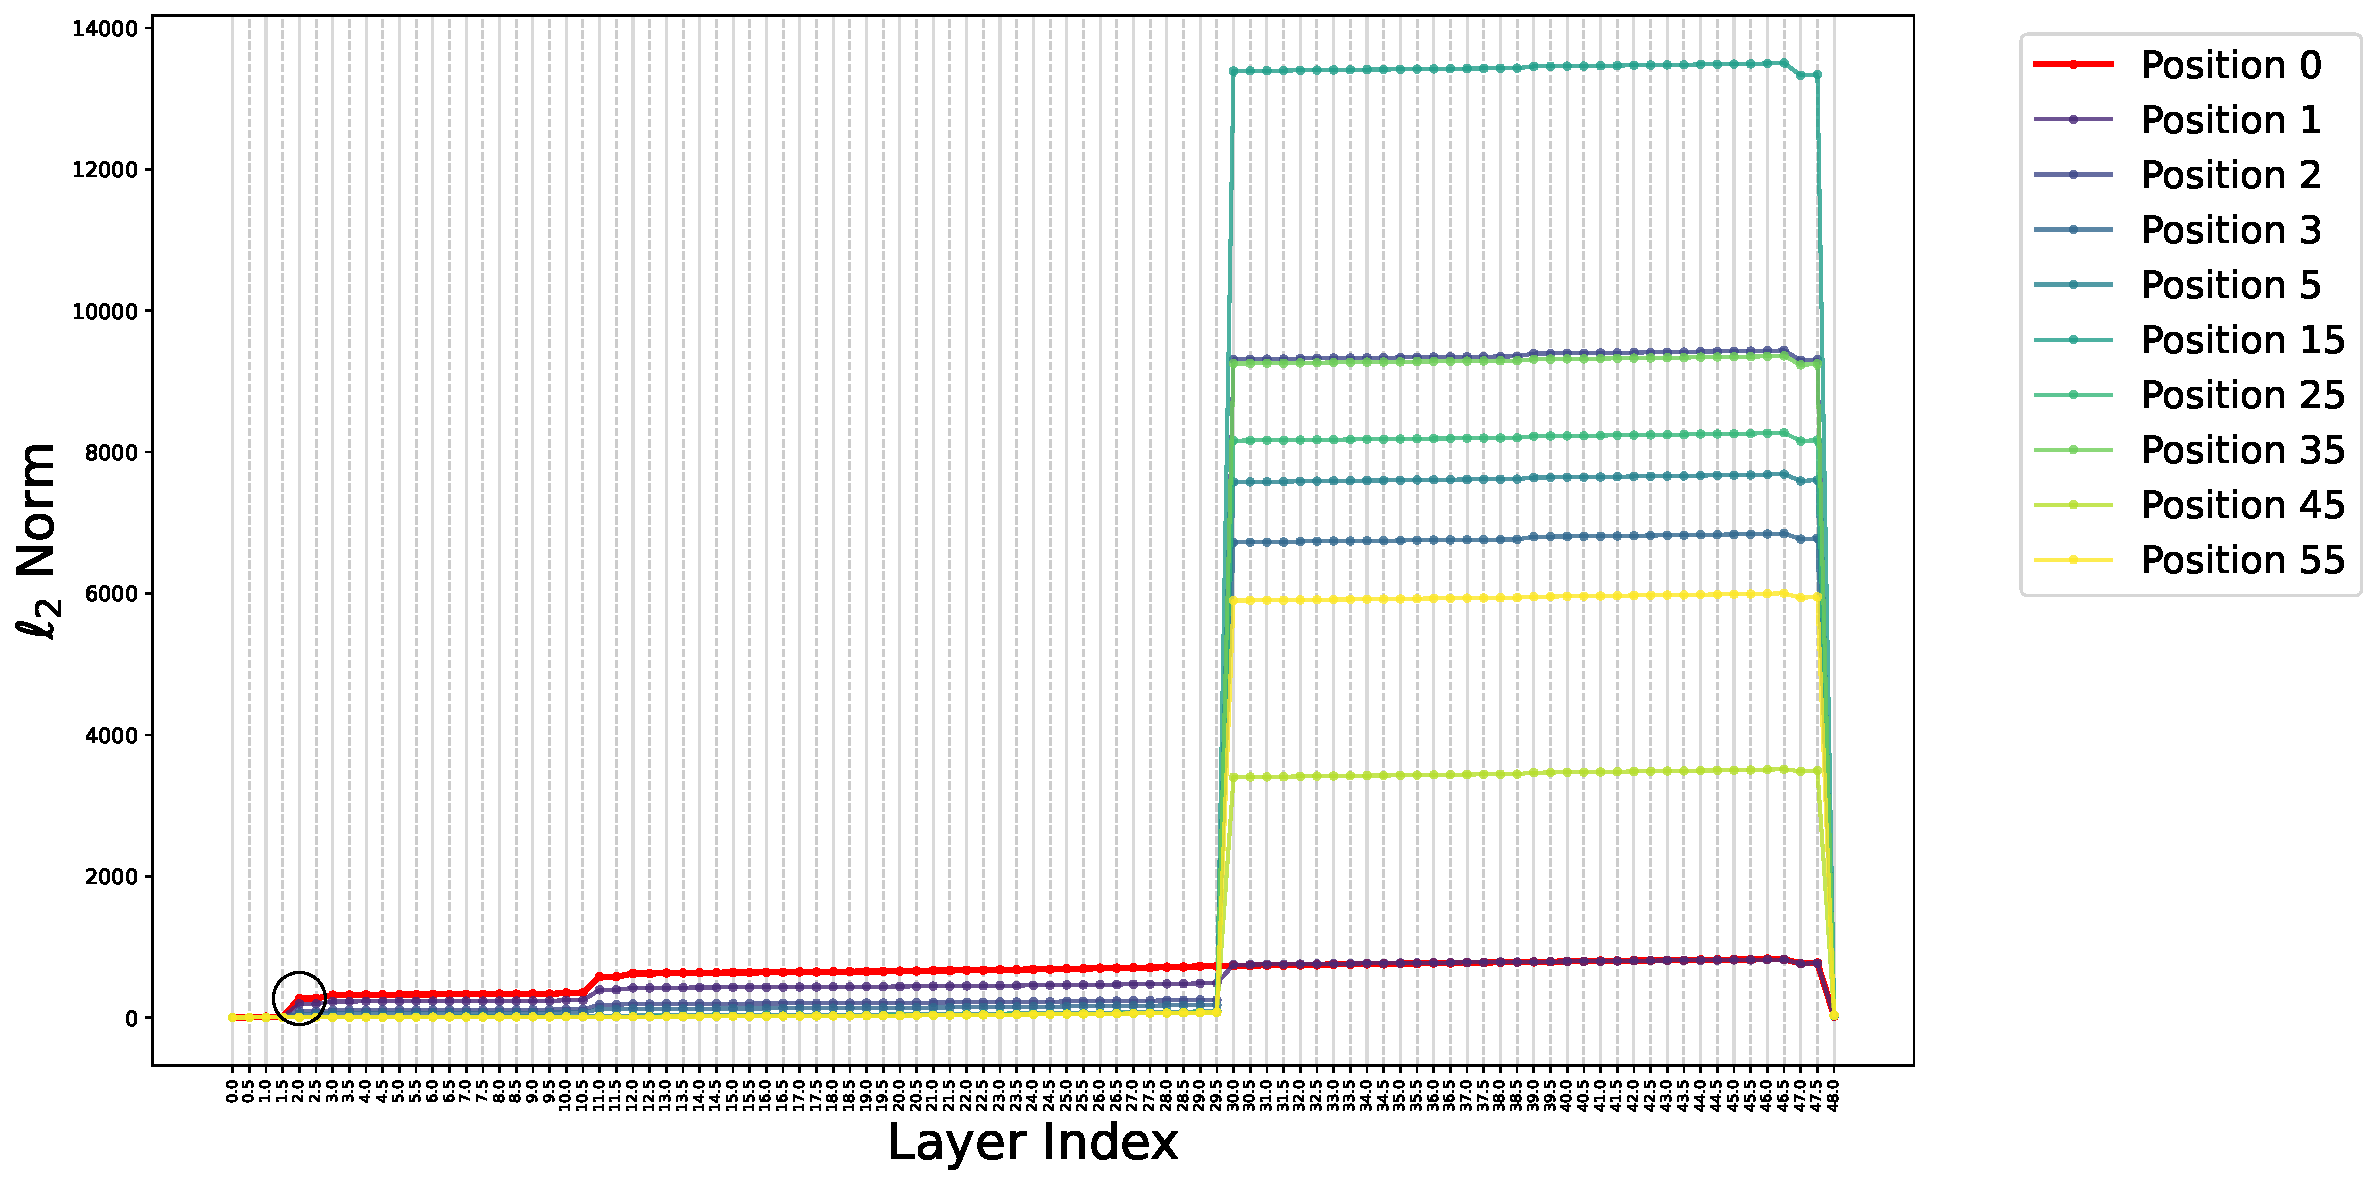
\includegraphics[width=0.95\columnwidth]{figures/fig6/fig6_step80000_l2norm.pdf}
    \end{subfigure}
    \begin{subfigure}[b]{0.95\linewidth} 
        \centering
        \caption{\scriptsize{Cosine Similarity to Position-Wise Mean}}
        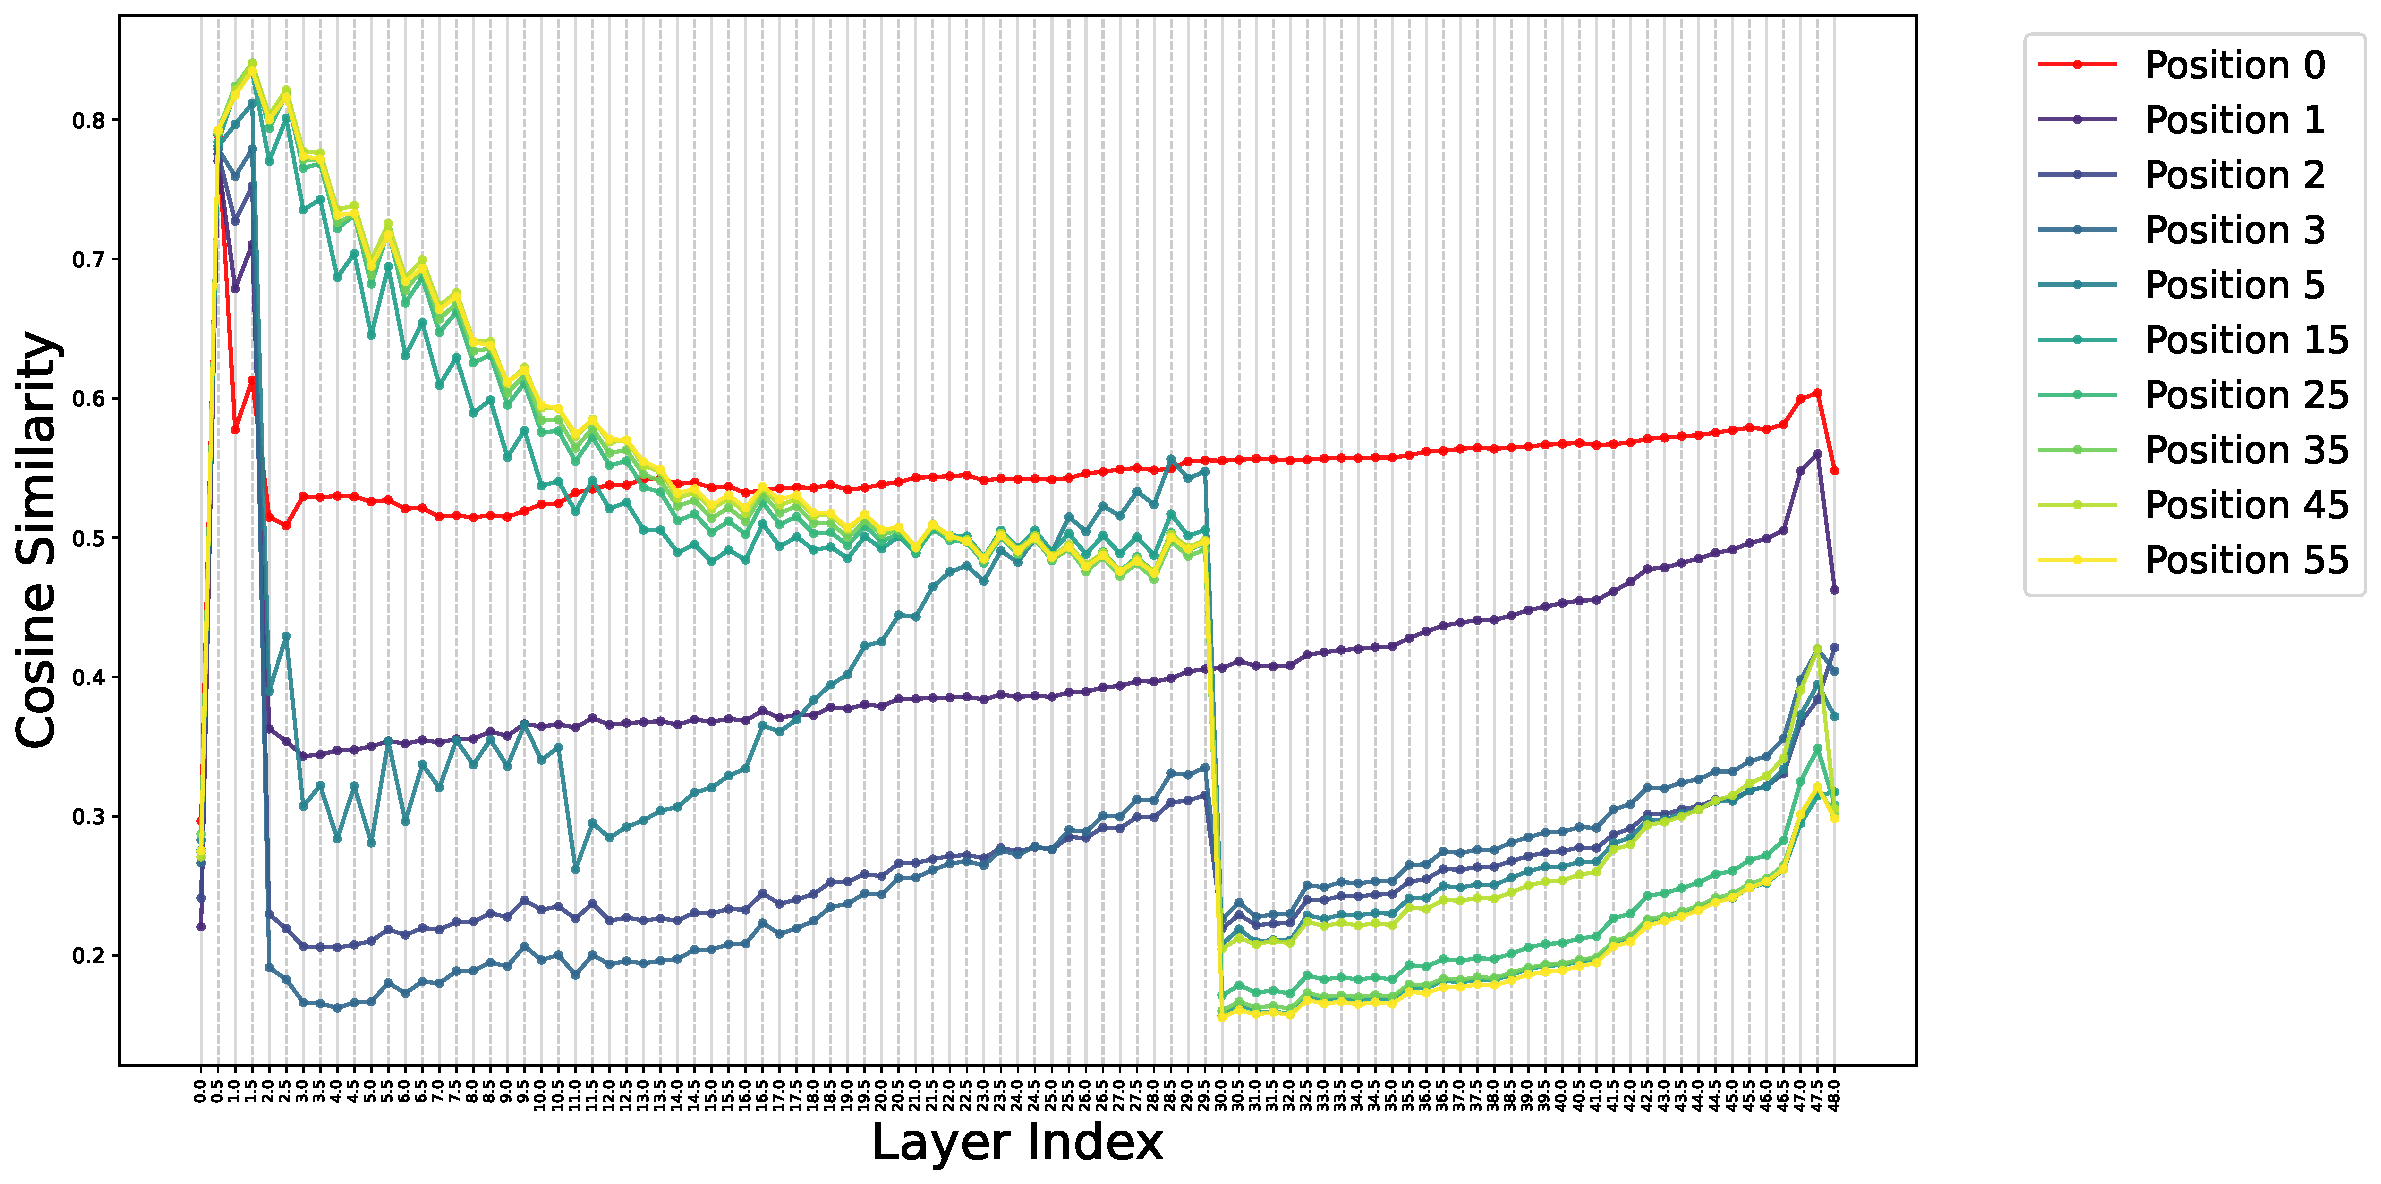
\includegraphics[width=0.95\columnwidth]{figures/fig6/fig6_step80000_sim.pdf}
    \end{subfigure}
    \begin{subfigure}[b]{0.95\linewidth} 
        \centering
        \caption{\scriptsize{Average Attention Score, Layer 2}}
        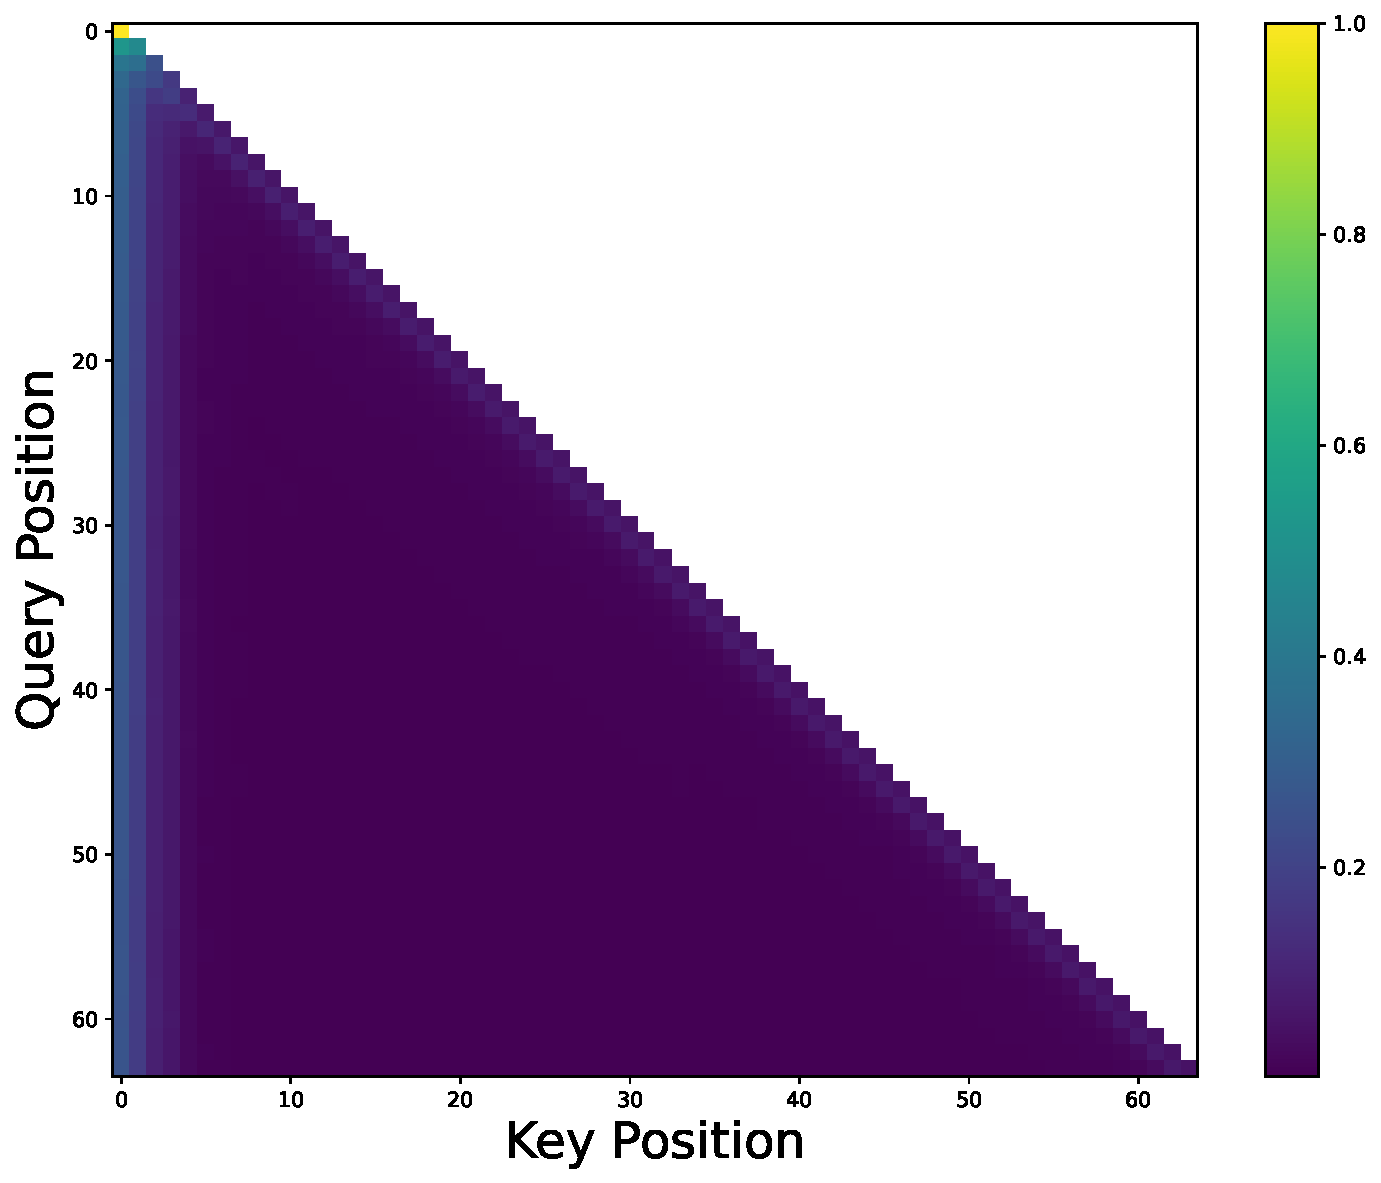
\includegraphics[width=0.7\columnwidth]{figures/fig6/fig6_step80000_layer2_attention.pdf}
    \end{subfigure}
\end{minipage}
\begin{minipage}[b]{0.32\linewidth} 
    \centering
    \begin{subfigure}[b]{0.95\linewidth} 
        \centering
        \caption{\scriptsize{Hidden States $\ell_2$Norm \\ Step 100000 ($\sim$780B Token)}}
        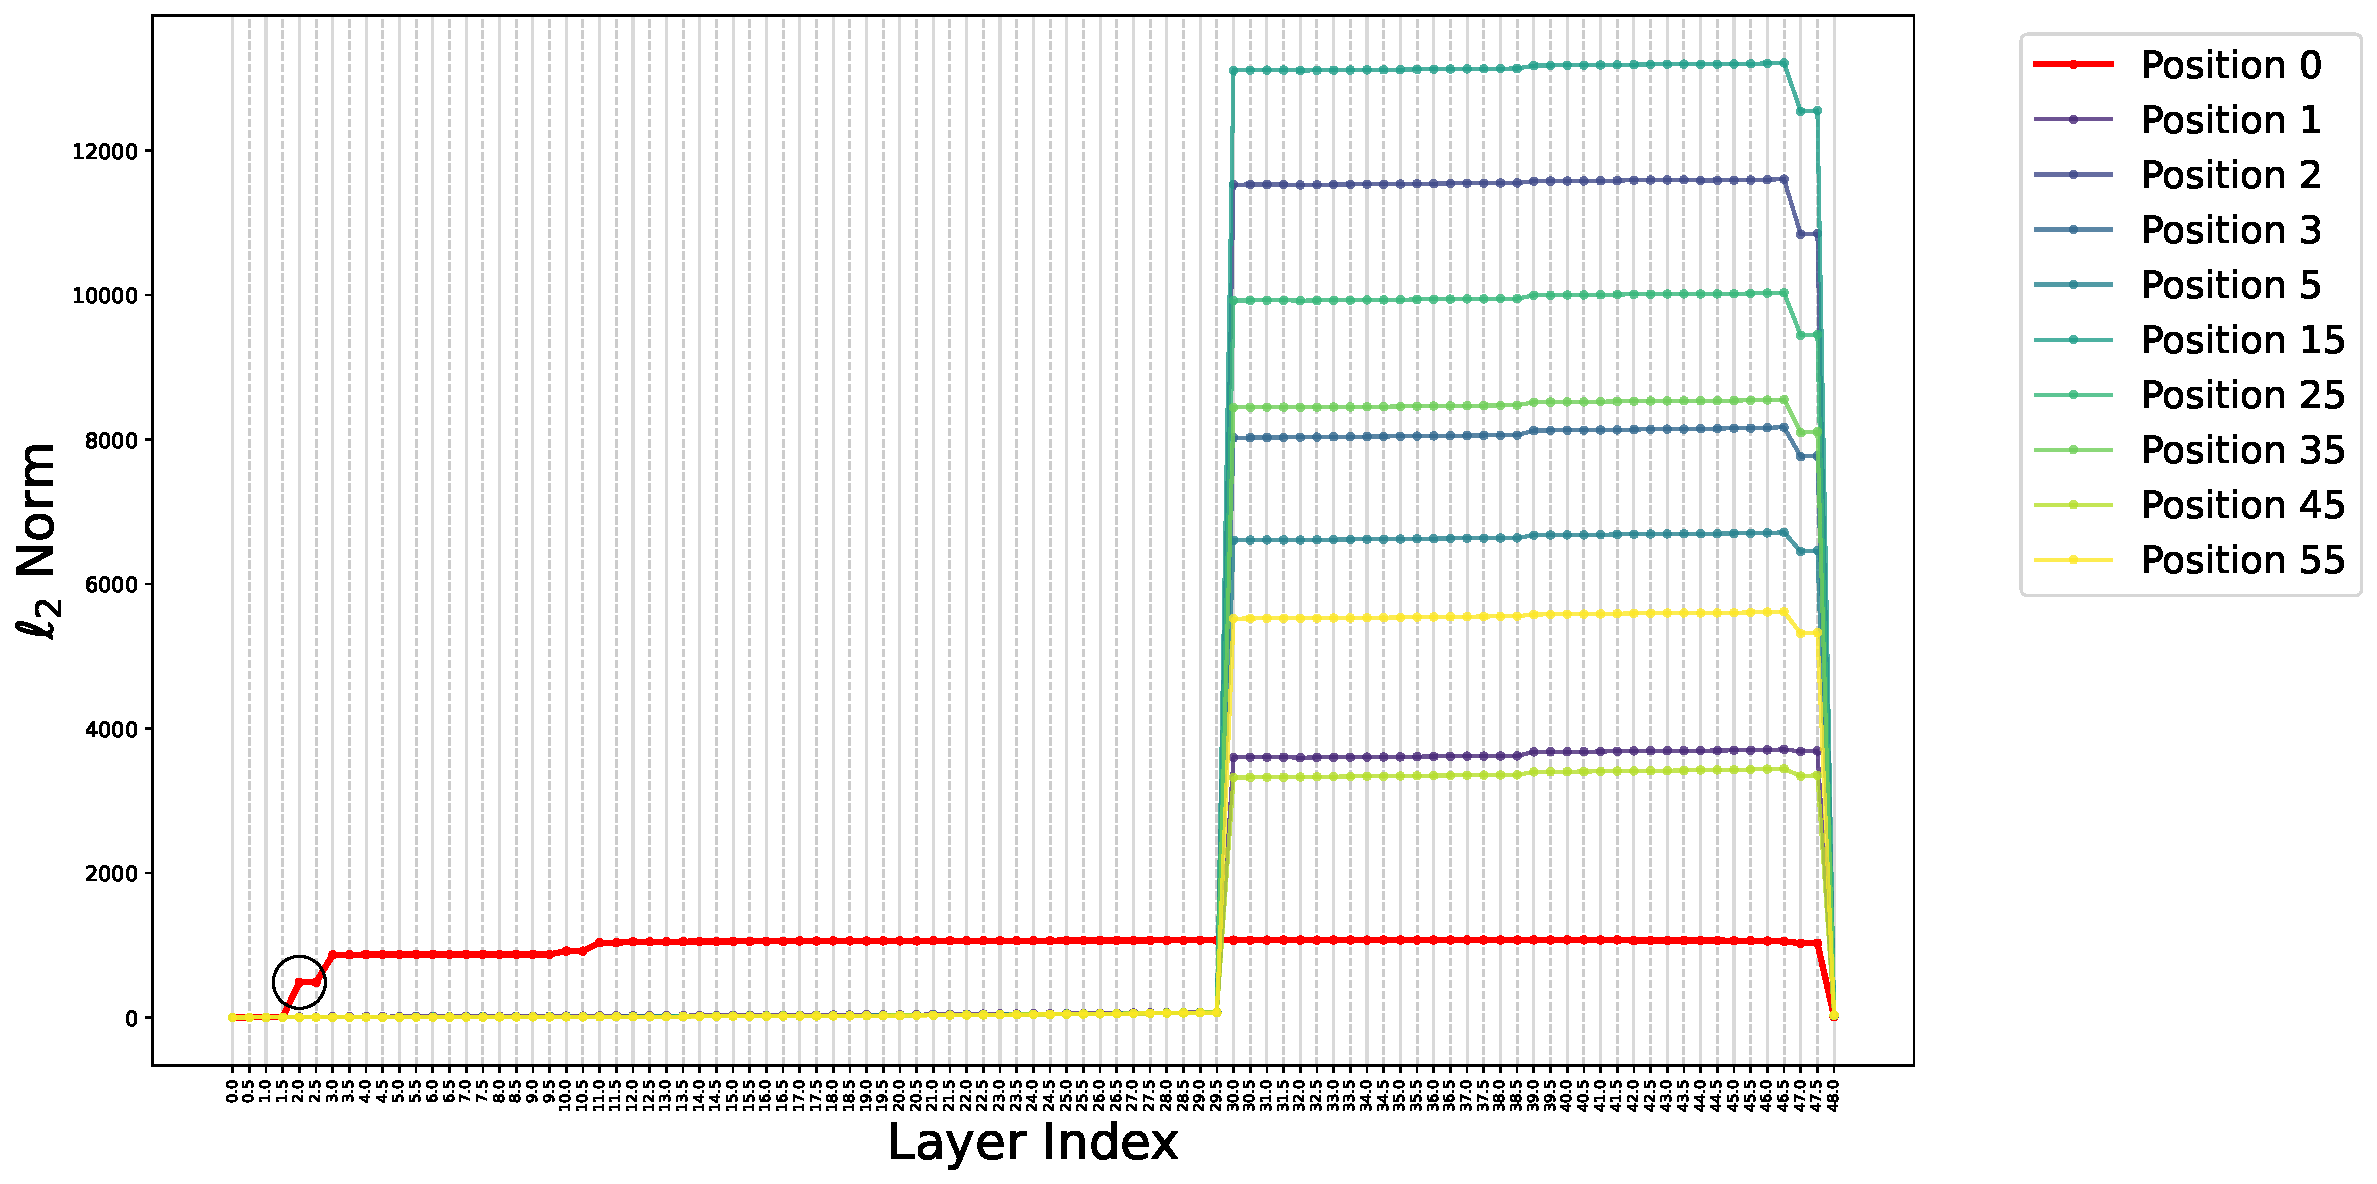
\includegraphics[width=0.95\columnwidth]{figures/fig6/fig6_step100000_l2norm.pdf}
    \end{subfigure}
    \begin{subfigure}[b]{0.95\linewidth} 
        \centering
        \caption{\scriptsize{Cosine Similarity to Position-Wise Mean}}
        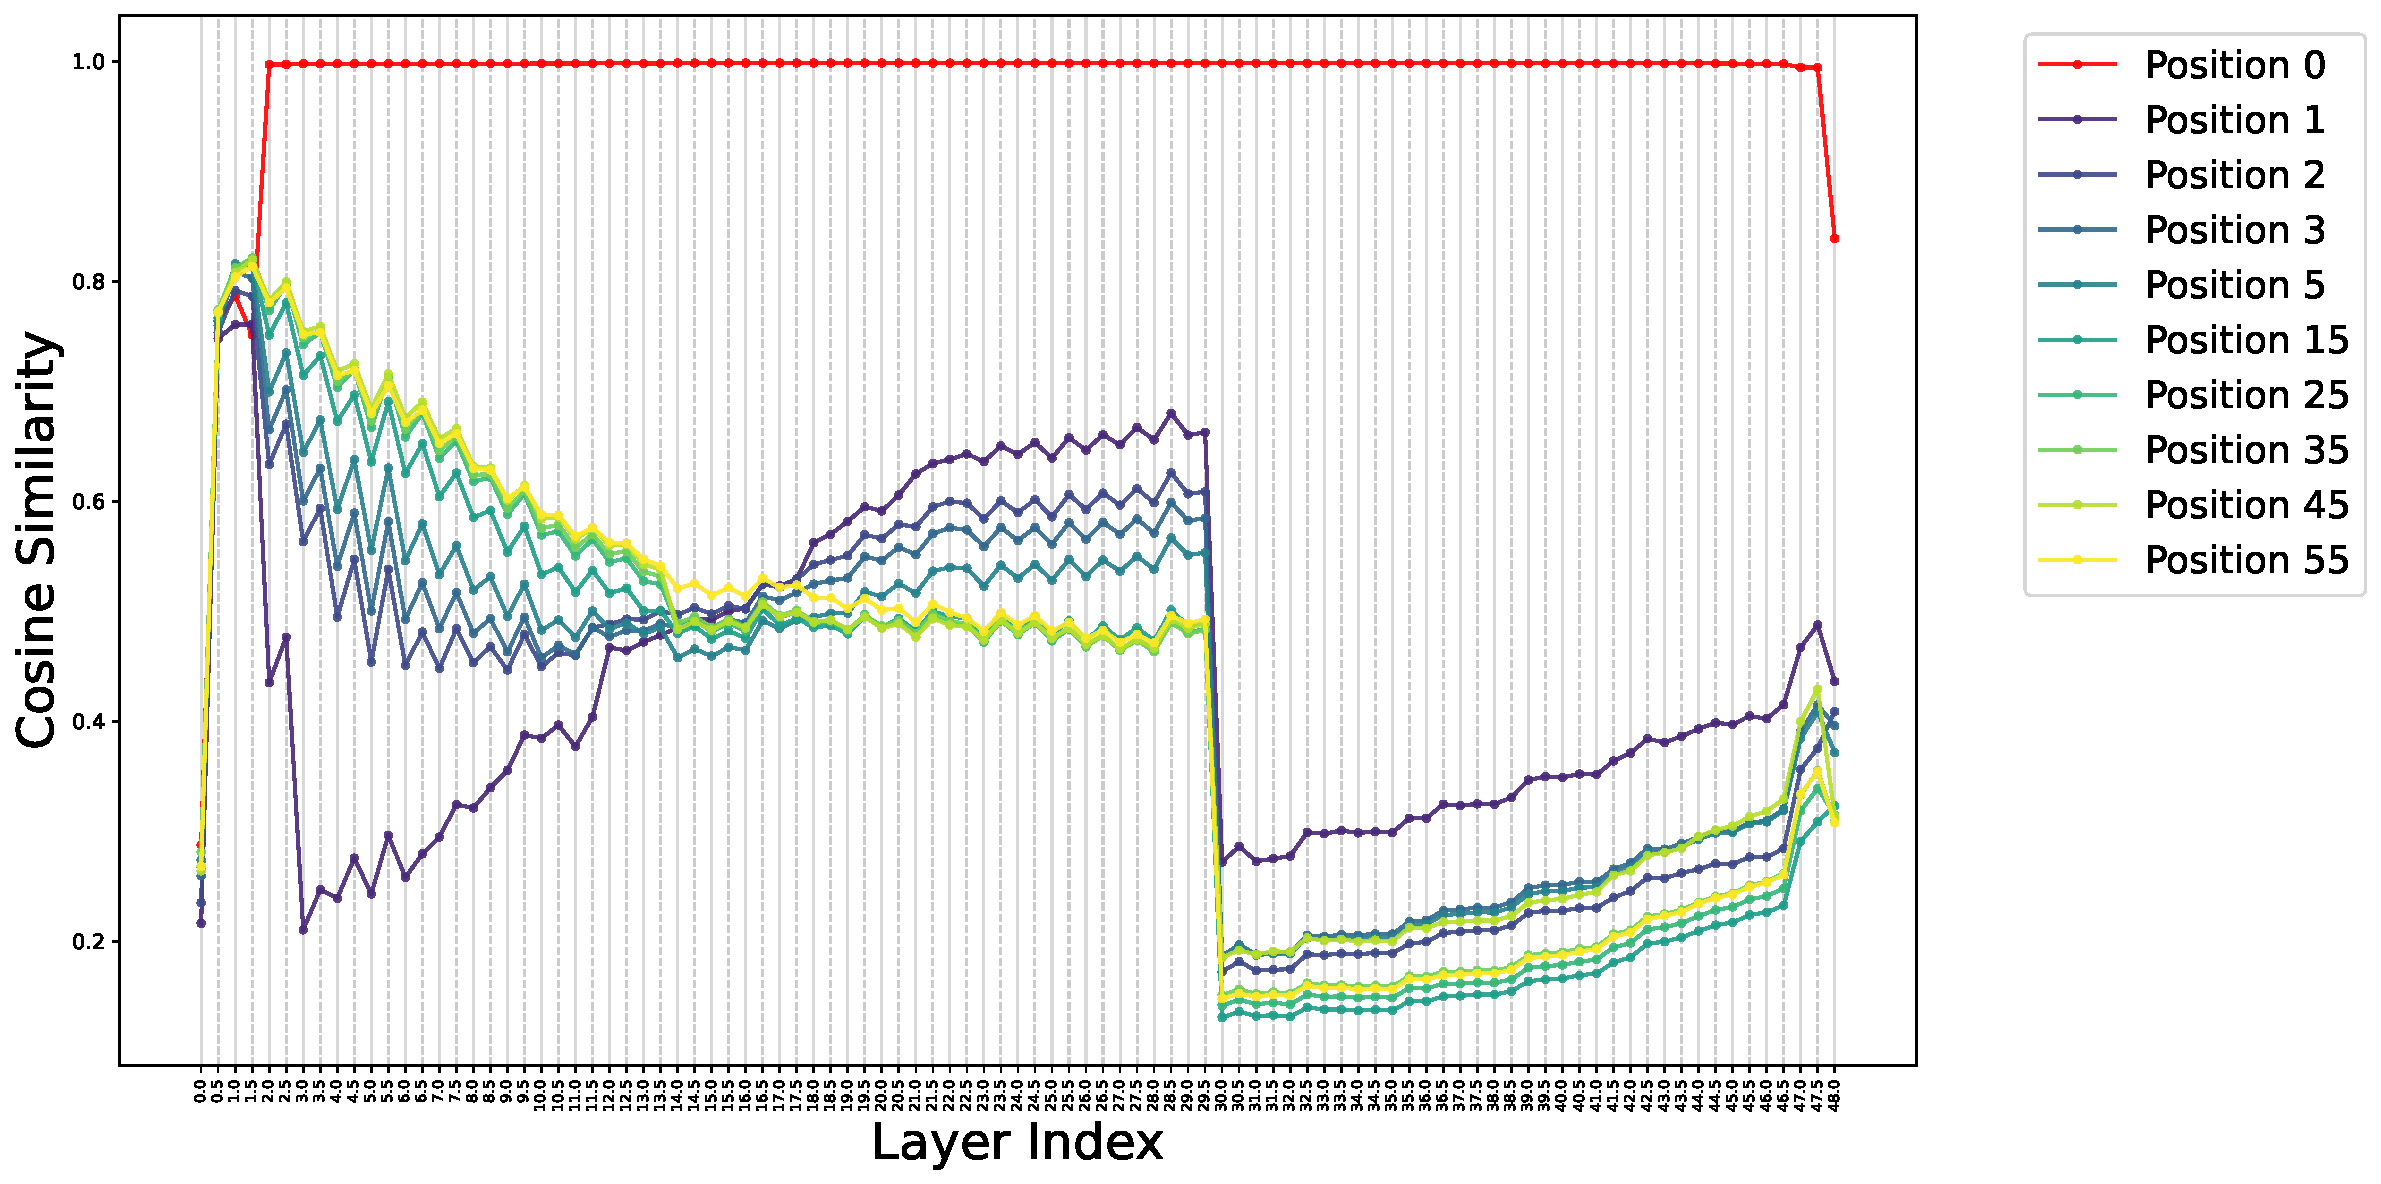
\includegraphics[width=0.95\columnwidth]{figures/fig6/fig6_step100000_sim.pdf}
    \end{subfigure}
    \begin{subfigure}[b]{0.95\linewidth} 
        \centering
        \caption{\scriptsize{Average Attention Score, Layer 2}}
        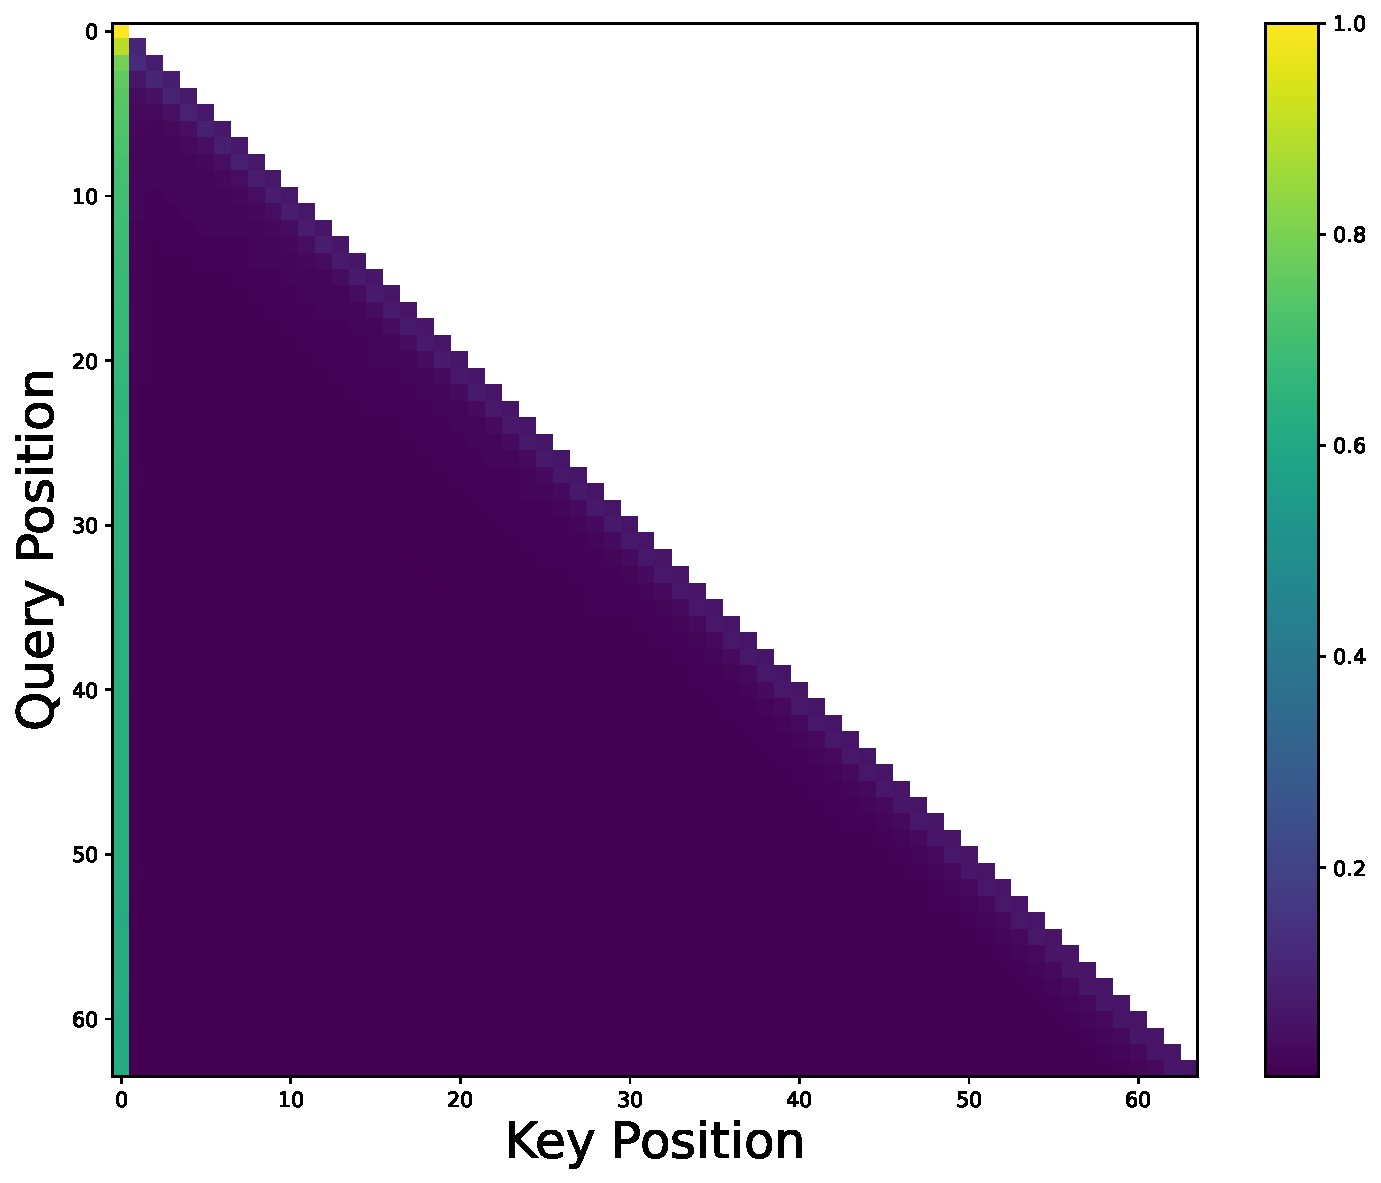
\includegraphics[width=0.7\columnwidth]{figures/fig6/fig6_step100000_layer2_attention.pdf}
    \end{subfigure}
\end{minipage}
\centering
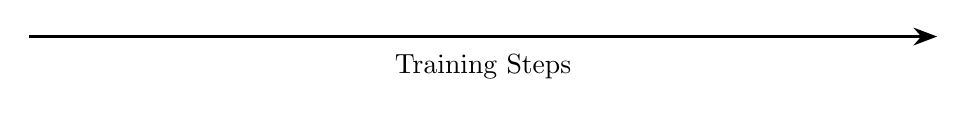
\begin{tikzpicture}
  \node[inner sep=0, minimum width=0.95\linewidth, minimum height=0pt] (box) {};
  \draw[-{Stealth[length=3mm]}, line width=0.98pt]
    (box.west) -- (box.east) node[midway, below=1mm] {Training Steps};
\end{tikzpicture}
\vspace{-1em}
\caption{Visualization of statistics during the Transitional Stage. The model temporarily shifts its sink center to position 1 as a transitional phase, before establishing a stable position-zero sink by forming an identification circuit for position 0.}
\vspace{-1em}
\label{fig-late-stage}
\end{figure*}

We have shown that a two-layer circuit is sufficient to induce a persistent position-zero sink that propagates to deeper layers. This naturally leads to the question: why do some models fail to form such a representation by the second layer? To explore this, we analyze training traces from a 30B-A3B MoE model trained from scratch \footnote{The model architecture and optimization hyperparameters follow those described in Qwen3 technical report~\citep{yang2025qwen3technicalreport}, with an enhanced version of Wanjuan-CC as the pretraining corpus~\cite{qiu2024wanjuanccsafehighqualityopensourced}.}. These traces offer insights into both the emergence and stabilization of the position-zero representation over the course of training.

For clarity, we divide the model’s training process into three distinct stages. In the \textbf{early stage}, a P0-Sink Circuit emerges in the middle layers of the model. However, this signal gradually fades and is replaced by a broader sink pattern that spans multiple positions. In the \textbf{transition stage}, the model temporarily relies on alternative tokens (e.g. position one) to form shallow, single-position sinks. These progressively shift and stabilize into a consistent position-zero sink within the shallow layers. The \textbf{final stage}, which we do not elaborate on in this work, is characterized by a fixed sink configuration that remains stable throughout the remainder of training.


\subsection{Early Stage}

As shown in Figure~\ref{fig-early-stage}, the P0-Sink Circuit emerges within the first 15B training tokens and initially appears in the middle layers of the network. This early emergence suggests that the mechanism benefits training by providing a favorable local optimum under language modeling objectives. While the P0 behavior remains the most prominent and stable, a similar but weaker pattern is also observed at position one. This observation supports our earlier analysis in Equation~\ref{eq:mixing}, which identifies relative averaging and position mixing, rather than explicit position-specific priors, as the underlying drivers of the sink effect.

This understanding also provides a concrete explanation for the drop in \textbf{Sink Rate} observed by \citet{barbero2025llmsattendtoken} when removing the \texttt{[BOS]} token from pretrained models. As defined by \citet{gu2025attentionsinkemergeslanguage}, the Sink Rate measures the proportion of attention heads and layers that allocate an average attention score above a moderate threshold $\varepsilon$ to a given token. \texttt{[BOS]}, the embedding vector of \texttt{[BOS]} facilitates early-layer sinks directly leading to elevated Sink Rates in shallow layers. When \texttt{[BOS]} is removed, models require deeper layers to build the \textbf{P0-Sink Circuit}, especially in the early stages of training where token exposure is limited. This results in a lower measured Sink Rate across the network.

However, such effects are no longer observed in more recent models. As modern LLMs are typically trained on significantly larger corpora, as stated in their official reports, even small models such as LLaMA-1B (shown in Figure~\ref{fig-llama1b}) are able to develop robust sink circuits within the first few layers. As a result, the absence of a \texttt{[BOS]} token has a diminishing impact on the observed Sink Rate.

At around 230B training tokens, the original P0 sink begins to fade. In its place, the model develops a broader sink pattern starting from layer 2, where attention is consistently concentrated on the early part of the input sequence. This pattern typically involves the first several tokens. Remarkably, this behavior persists through all subsequent layers and remains stable until at least 460B tokens.
In this stage, the attention pattern closely mirrors those observed in StreamingLLM~\citep{xiao2024efficientstreaminglanguagemodels}, where the initial tokens are expected to function as persistent context anchors. The structural similarity suggests that this broad-spectrum sink may serve a similar role, facilitating stable context accumulation in long sequences and supporting efficient autoregressive processing.


During training, we also observe a distinct phenomenon in the deeper layers. After layer 30, certain activations become abnormally large and exhibit clear position-dependent patterns. However, as shown in the visualizations in Appendix~\ref{appendix-ckpt-attn}, the corresponding attention scores remain largely unaffected. 
% These activations appear to be only weakly related to the P0 sink mechanism discussed earlier. Instead, they may reflect the model’s attempt to reorient specific hidden states in order to reduce their similarity across positions. According to Equation~\ref{eq:norm}, this behavior likely arises from the model amplifying certain features at specific positions in order to minimize changes to the normalized representations. 
Since this effect does not directly impact the attention mechanism and falls outside the main scope of our study, we leave a detailed analysis to future work and restrict our focus to the earlier layers, where the sink mechanism more clearly emerges.

\subsection{Transitional Stage}

After a prolonged phase dominated by a broad-spectrum sink pattern, the influence of the initial position-zero circuit gradually diminishes. One possible explanation is that the earlier layers begin to transition into a form of sink-based attention that enables head-level gating control, as discussed by~\citet{sandovalsegura2025identifyingevaluatinginactiveheads}. The model subsequently shifts its sink center from position zero to position one. Notably, this new sink emerges earlier in the network, beginning at layer 2, as illustrated in Figure~\ref{fig7c}. In this context, we use the term \textit{sink center} to refer to the token position whose hidden states are most consistently clustered and reinforced across layers, thereby serving as a persistent anchor for attention throughout the model.

As shown in Figure~\ref{fig-late-stage}, the model attempts to identify commonalities among position-one tokens and cluster their hidden states into a consistent representation, thereby establishing a stable sink at position one. However, this configuration proves to be transient. After only a modest number of additional training steps, the sink shifts back to position zero and persists there through later stages of training.

This shift can be explained by the structural asymmetry formalized in Equation~\ref{eq:mixing}. Under causal attention, position zero is inherently more invariant to input variation, as it attends only to itself. In contrast, position one aggregates signals from both itself and position zero, resulting in a representation that is more context-dependent and therefore more difficult to align across different inputs. This structural advantage renders position zero more suitable for amplification into a stable attention sink. As a result, the model eventually reestablishes the position-zero sink, which then remains consistent throughout the remainder of training.

\subsection{Implications and Applications}

Based on the observed phenomena associated with the position-zero sink, we hypothesize that the stage at which this sink circuit stabilizes, whether it is the early stage, the transitional stage, or the final stage, can serve as an indicator of the model’s pretraining convergence status. It is important to note that reaching a later stage does not necessarily imply stronger performance. Instead, the sink stage reflects the model’s position within the pretraining trajectory. If post-training is initiated while the model remains in an earlier sink stage, continued pretraining may lead to improved downstream performance. We provide further analysis in Appendix~\ref{appendix-recentllm}.

\section{Conclusion}

In this work, we study how position-zero attention sinks arise and persist in modern large language models. We show that while the \texttt{[BOS]} token contributes to sink behavior in shallow layers for models trained with it, a robust position-zero sink persist in deeper layers even after removing \texttt{[BOS]}, indicating that the sink phenomenon is not reducible to token embeddings.

We further identify a simple and generalizable two-block transformer circuit that enables the model to recognize position zero tokens and amplify the $\ell_2$ norm of its hidden state, thereby stabilizing the sink pattern across layers. By tracing training dynamics in a 30B-parameter model with 3B activated parameters trained from scratch, we show that this \textbf{P0-Sink Circuit} emerges early and becomes concentrated in the first two layers over time.

These findings reveal the mechanism behind attention sink emergence and offer a diagnostic signal for estimating training stage and convergence. More broadly, they highlight implicit architectural biases in transformers and suggest directions for improving interpretability, efficiency, and stability in future designs.

\section*{Impact Statement}
% This paper presents work whose goal is to advance the field of Machine Learning. There are many potential societal consequences of our work, none which we feel must be specifically highlighted here.

\clearpage
\bibliographystyle{plainnat}
\bibliography{example_paper}


%%%%%%%%%%%%%%%%%%%%%%%%%%%%%%%%%%%%%%%%%%%%%%%%%%%%%%%%%%%%

\clearpage
%%%%%%%%%%%%%%%%%%%%%%%%%%%%%%%%%%%%%%%%%%%%%%%%%%%%%%%%%%%%%%%%%%%%%%%%%%%%%%%
%%%%%%%%%%%%%%%%%%%%%%%%%%%%%%%%%%%%%%%%%%%%%%%%%%%%%%%%%%%%%%%%%%%%%%%%%%%%%%%
% APPENDIX
%%%%%%%%%%%%%%%%%%%%%%%%%%%%%%%%%%%%%%%%%%%%%%%%%%%%%%%%%%%%%%%%%%%%%%%%%%%%%%%
%%%%%%%%%%%%%%%%%%%%%%%%%%%%%%%%%%%%%%%%%%%%%%%%%%%%%%%%%%%%%%%%%%%%%%%%%%%%%%%
\newpage
\appendix
\onecolumn

\section{Dataset and Setup}

Unless otherwise specified (e.g., Table~\ref{bos-vs-non-bos-tab2}), all experiments in this paper are conducted on a 10B-token subset of the FineWeb-Edu dataset, specifically using the first 1024 samples from the first \texttt{.parquet} file, with a maximum sequence length of 64.

\section{Checkpoint Attention Heatmap}
\label{appendix-ckpt-attn}

\begin{figure*}[h]
    \begin{subfigure}[b]{0.33\linewidth} 
        \caption{\scriptsize{Layer 31}}
        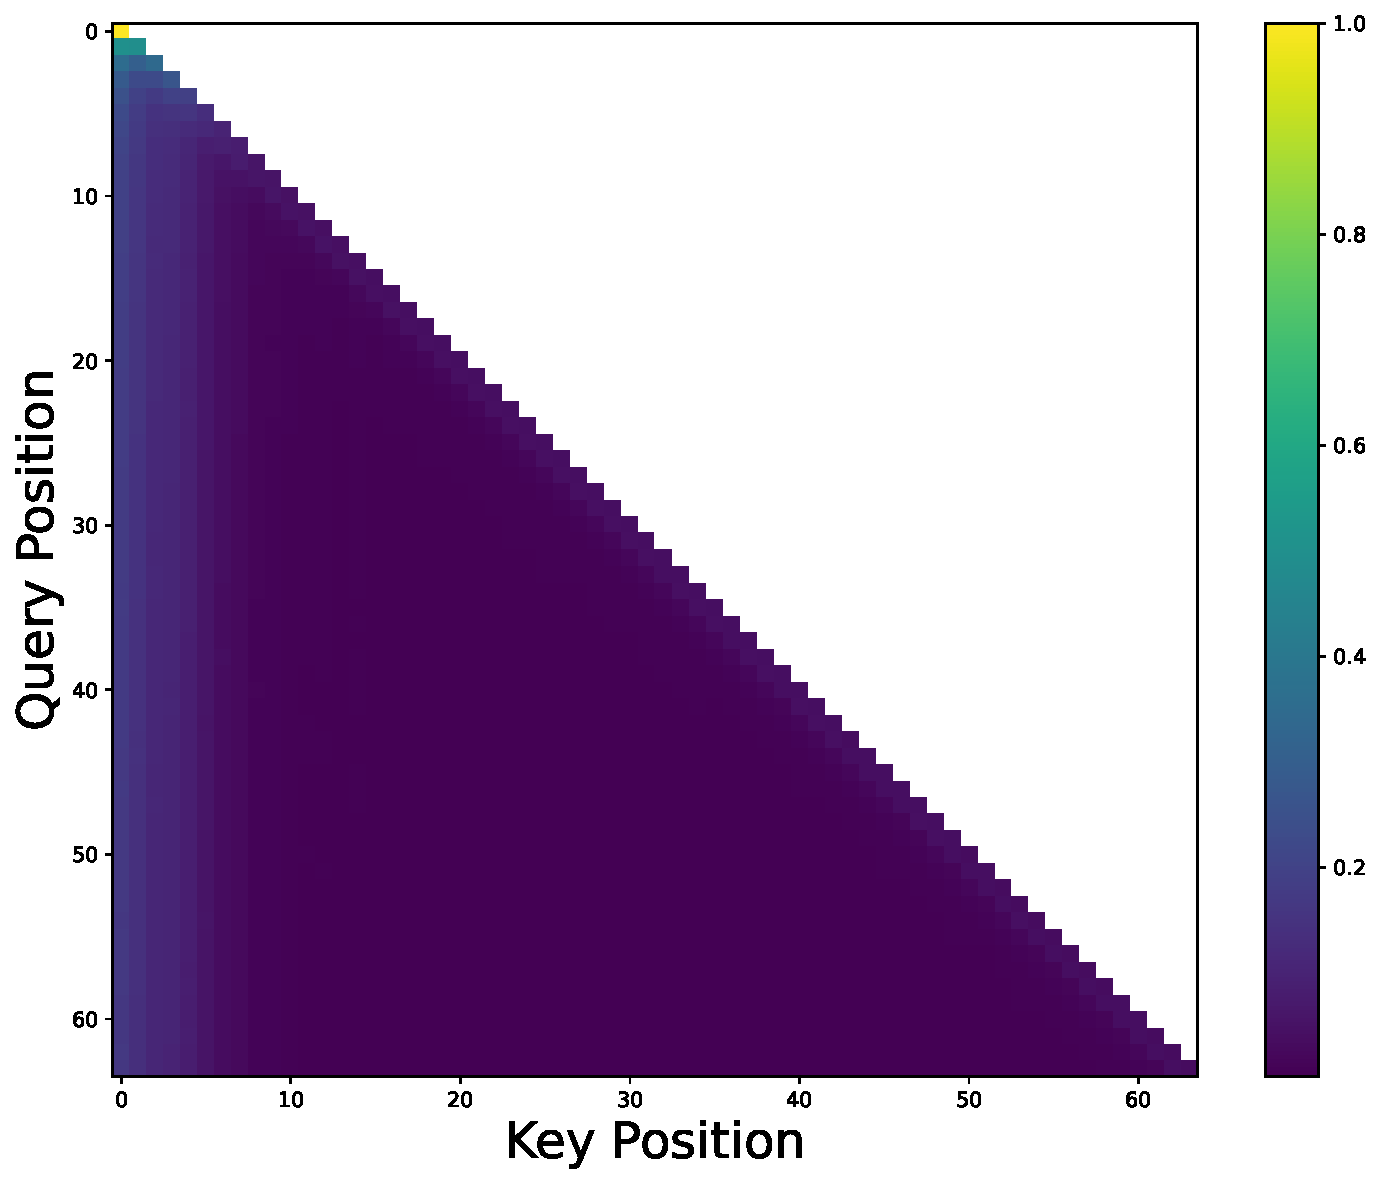
\includegraphics[width=\columnwidth]{figures/appendixA/layer31_attention.pdf}
    \end{subfigure}
    \begin{subfigure}[b]{0.33\linewidth} 
        \caption{\scriptsize{Layer 32}}
        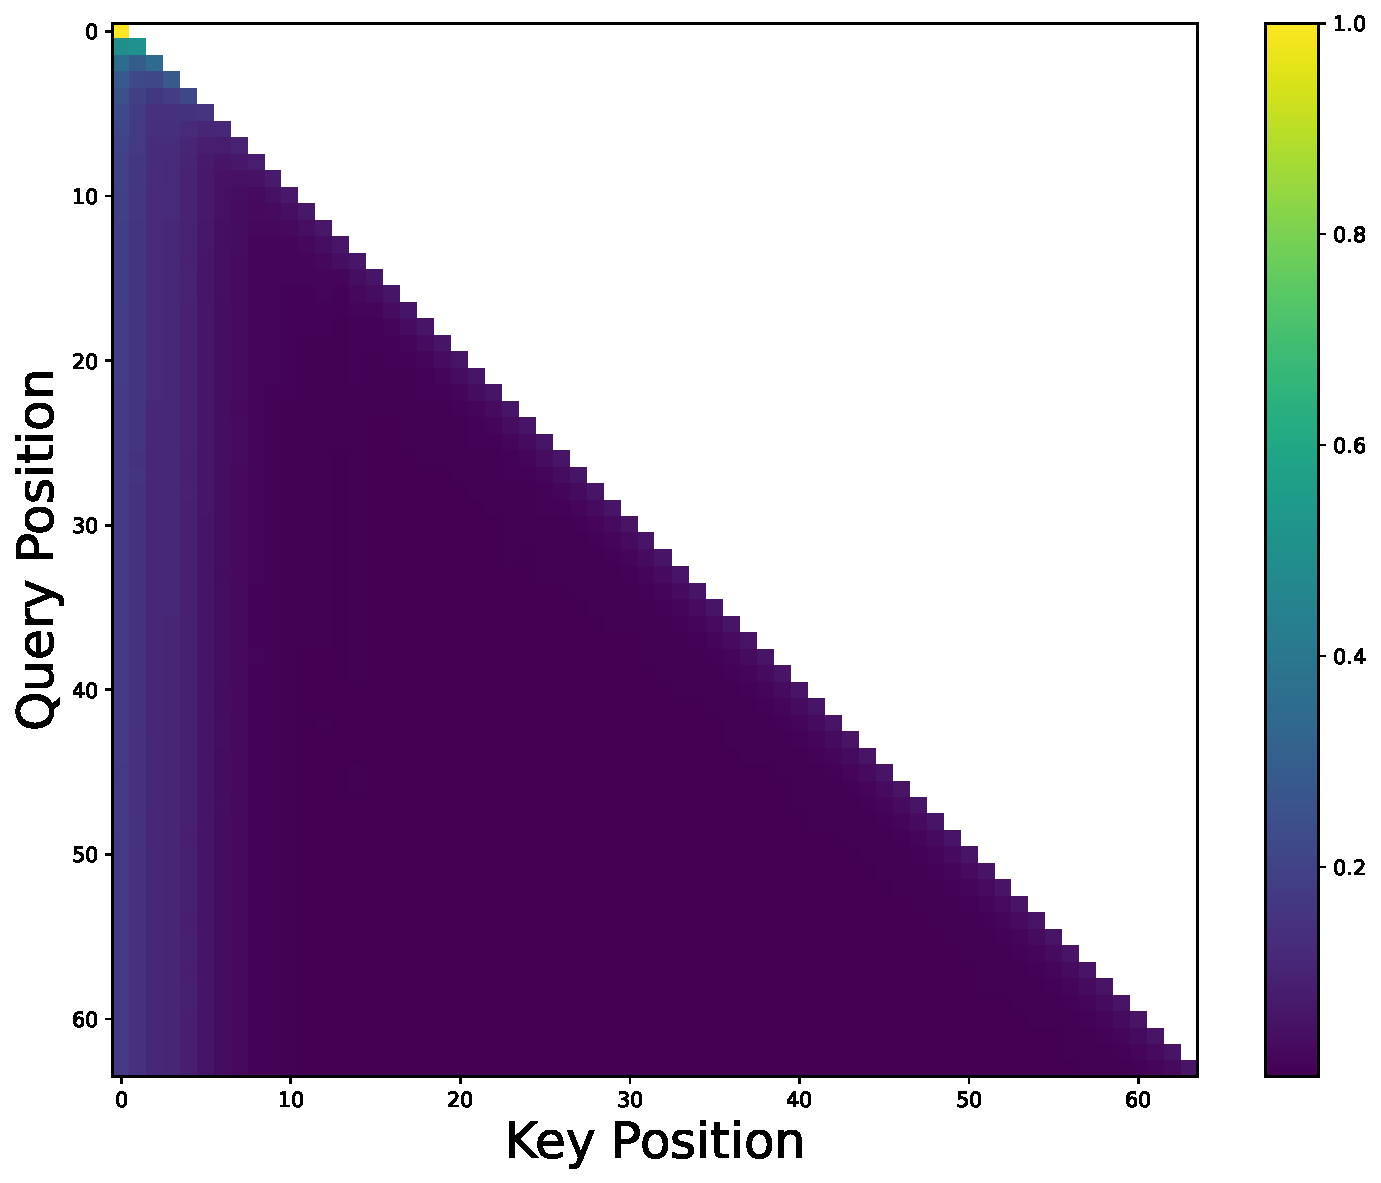
\includegraphics[width=\columnwidth]{figures/appendixA/layer32_attention.pdf}
    \end{subfigure}
    \begin{subfigure}[b]{0.33\linewidth} 
        \caption{\scriptsize{Layer 33}}
        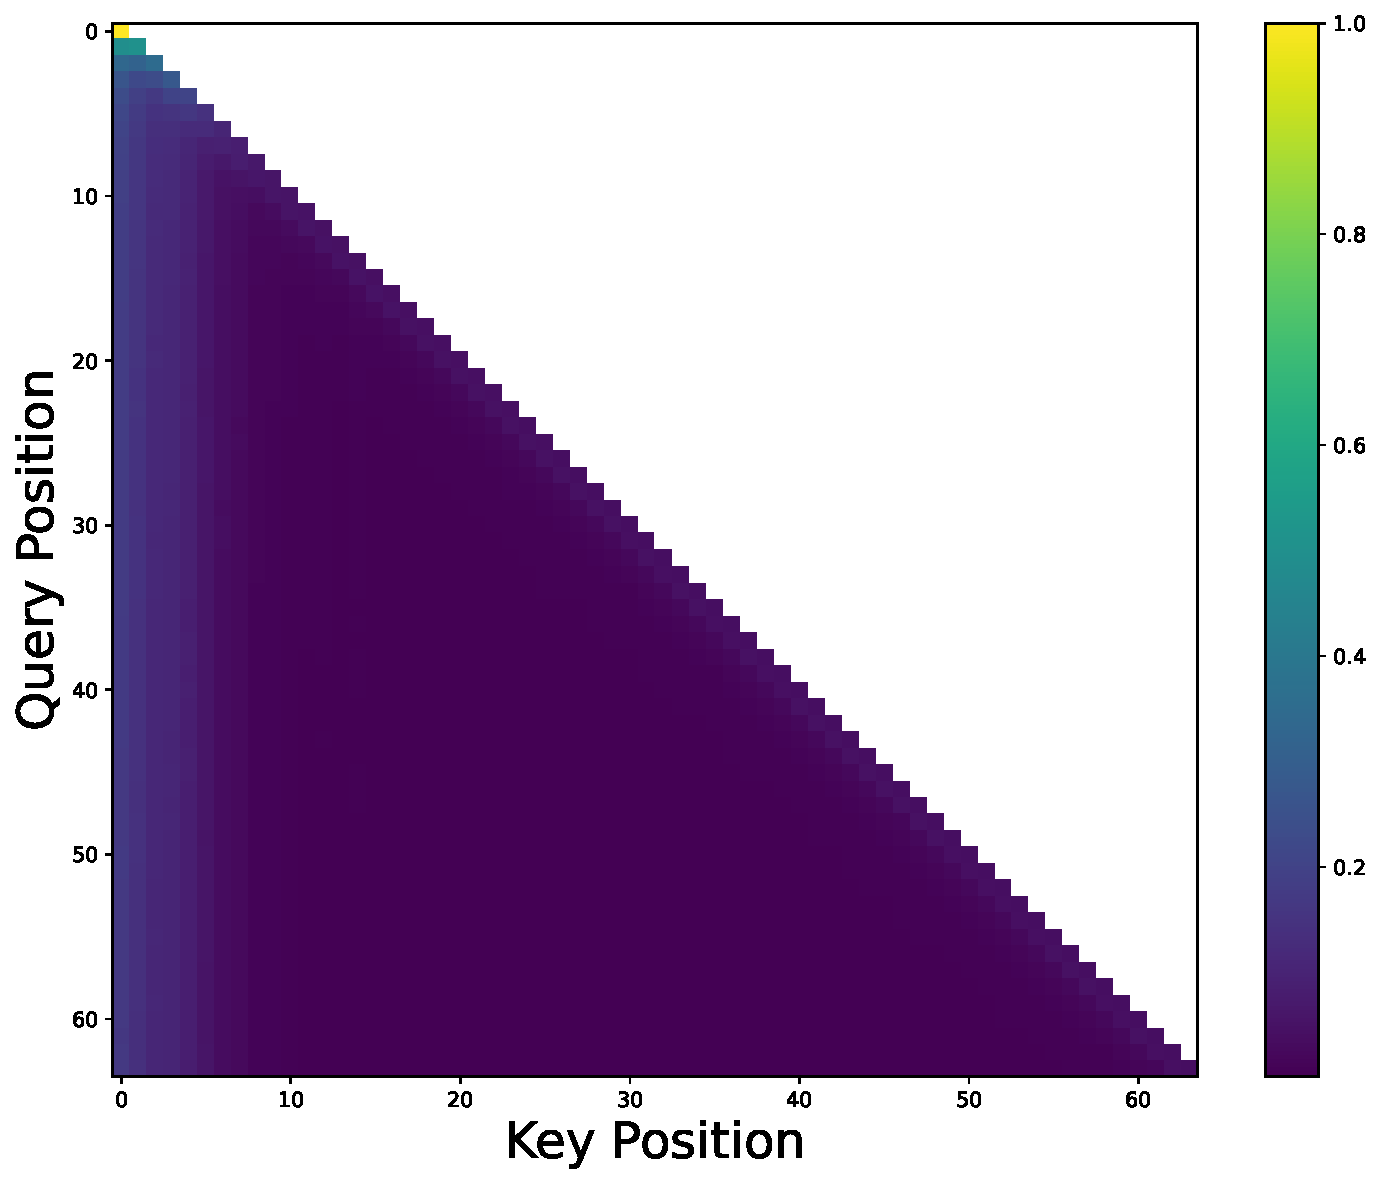
\includegraphics[width=\columnwidth]{figures/appendixA/layer33_attention.pdf}
    \end{subfigure}
    \begin{subfigure}[b]{0.33\linewidth} 
        \caption{\scriptsize{Layer 34}}
        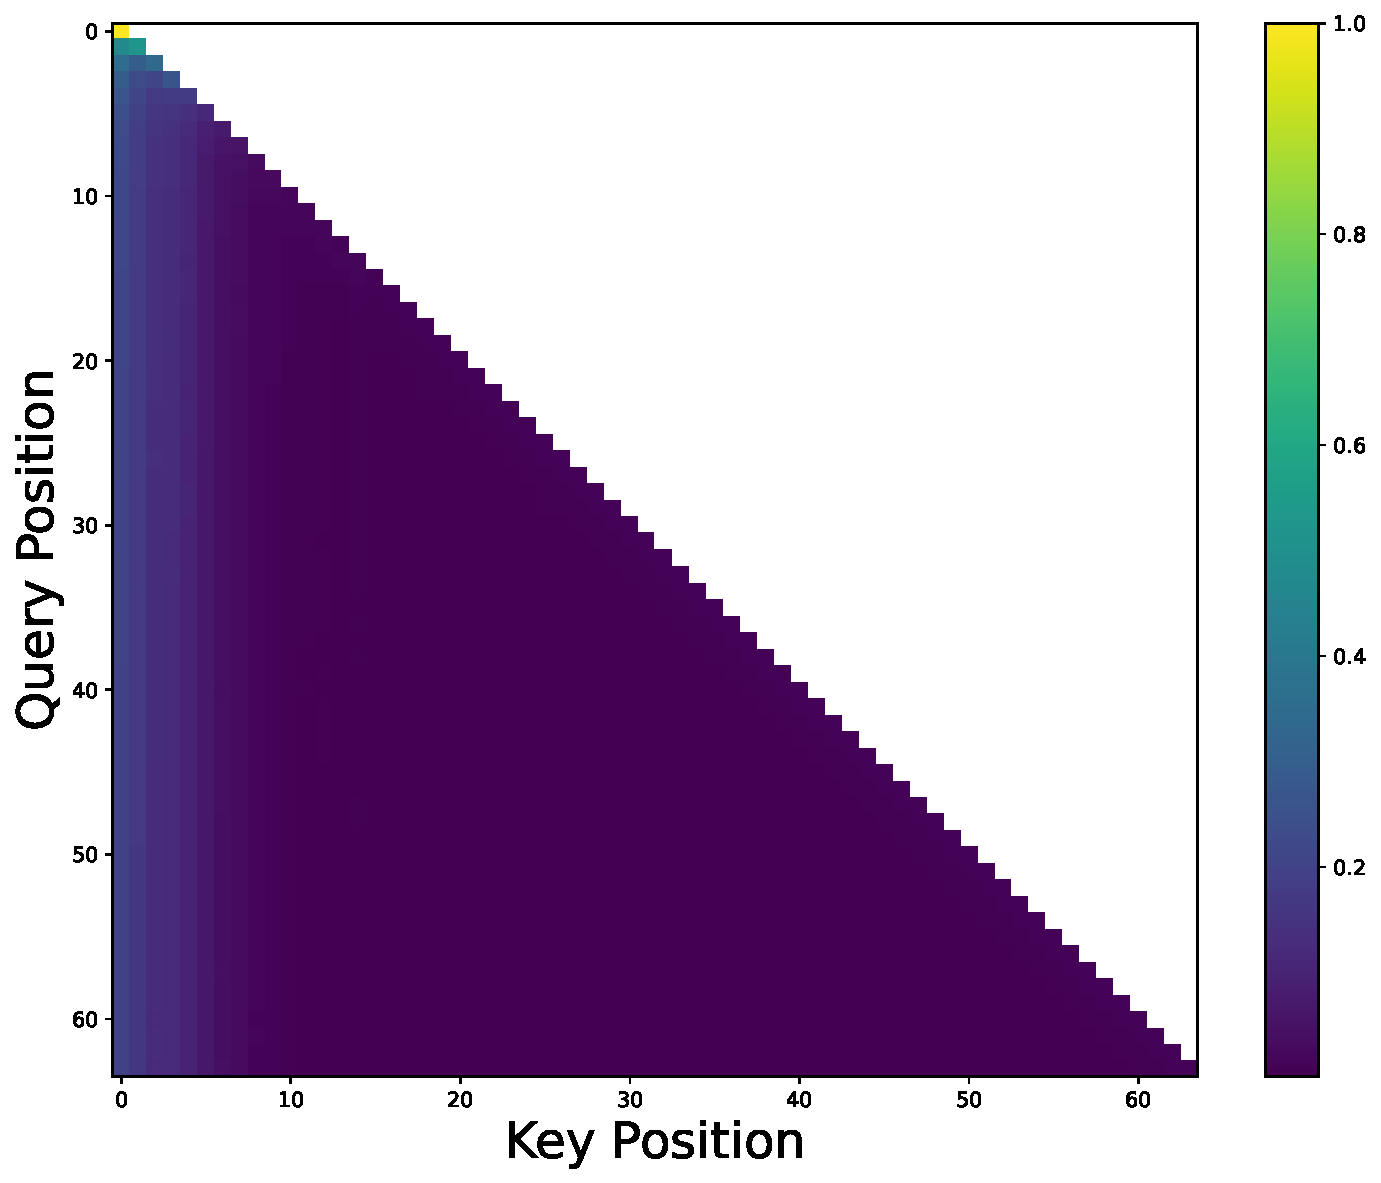
\includegraphics[width=\columnwidth]{figures/appendixA/layer34_attention.pdf}
    \end{subfigure}
    \begin{subfigure}[b]{0.33\linewidth} 
        \caption{\scriptsize{Layer 35}}
        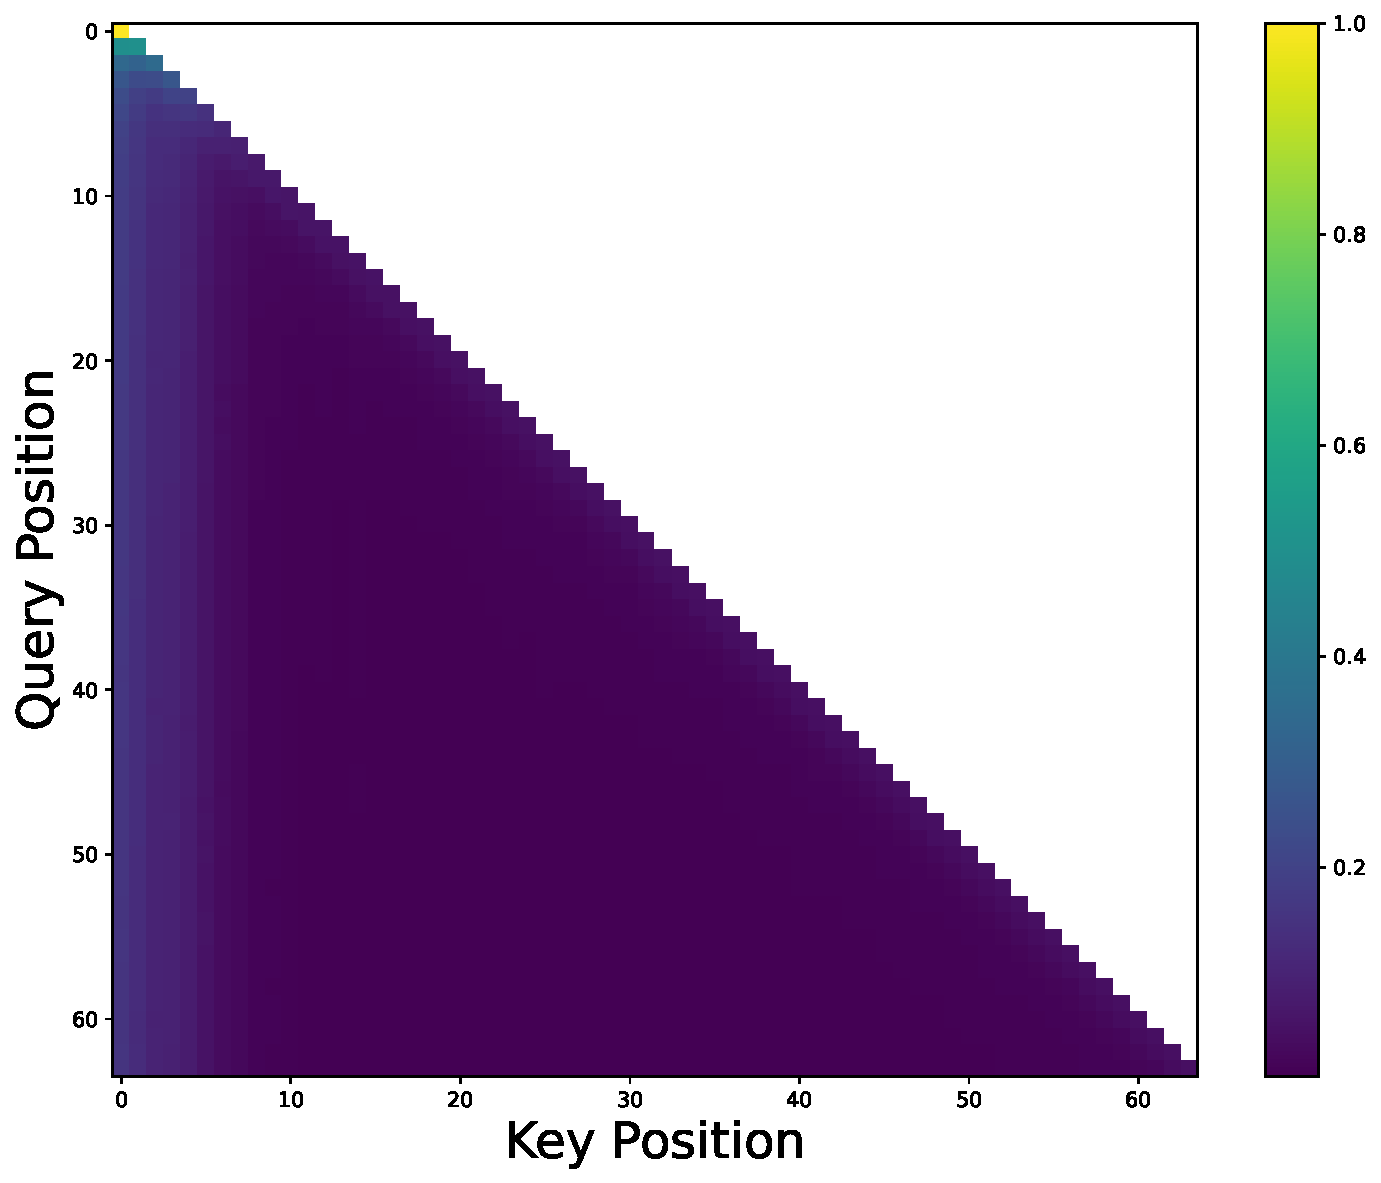
\includegraphics[width=\columnwidth]{figures/appendixA/layer35_attention.pdf}
    \end{subfigure}
    \begin{subfigure}[b]{0.33\linewidth} 
        \caption{\scriptsize{Layer 36}}
        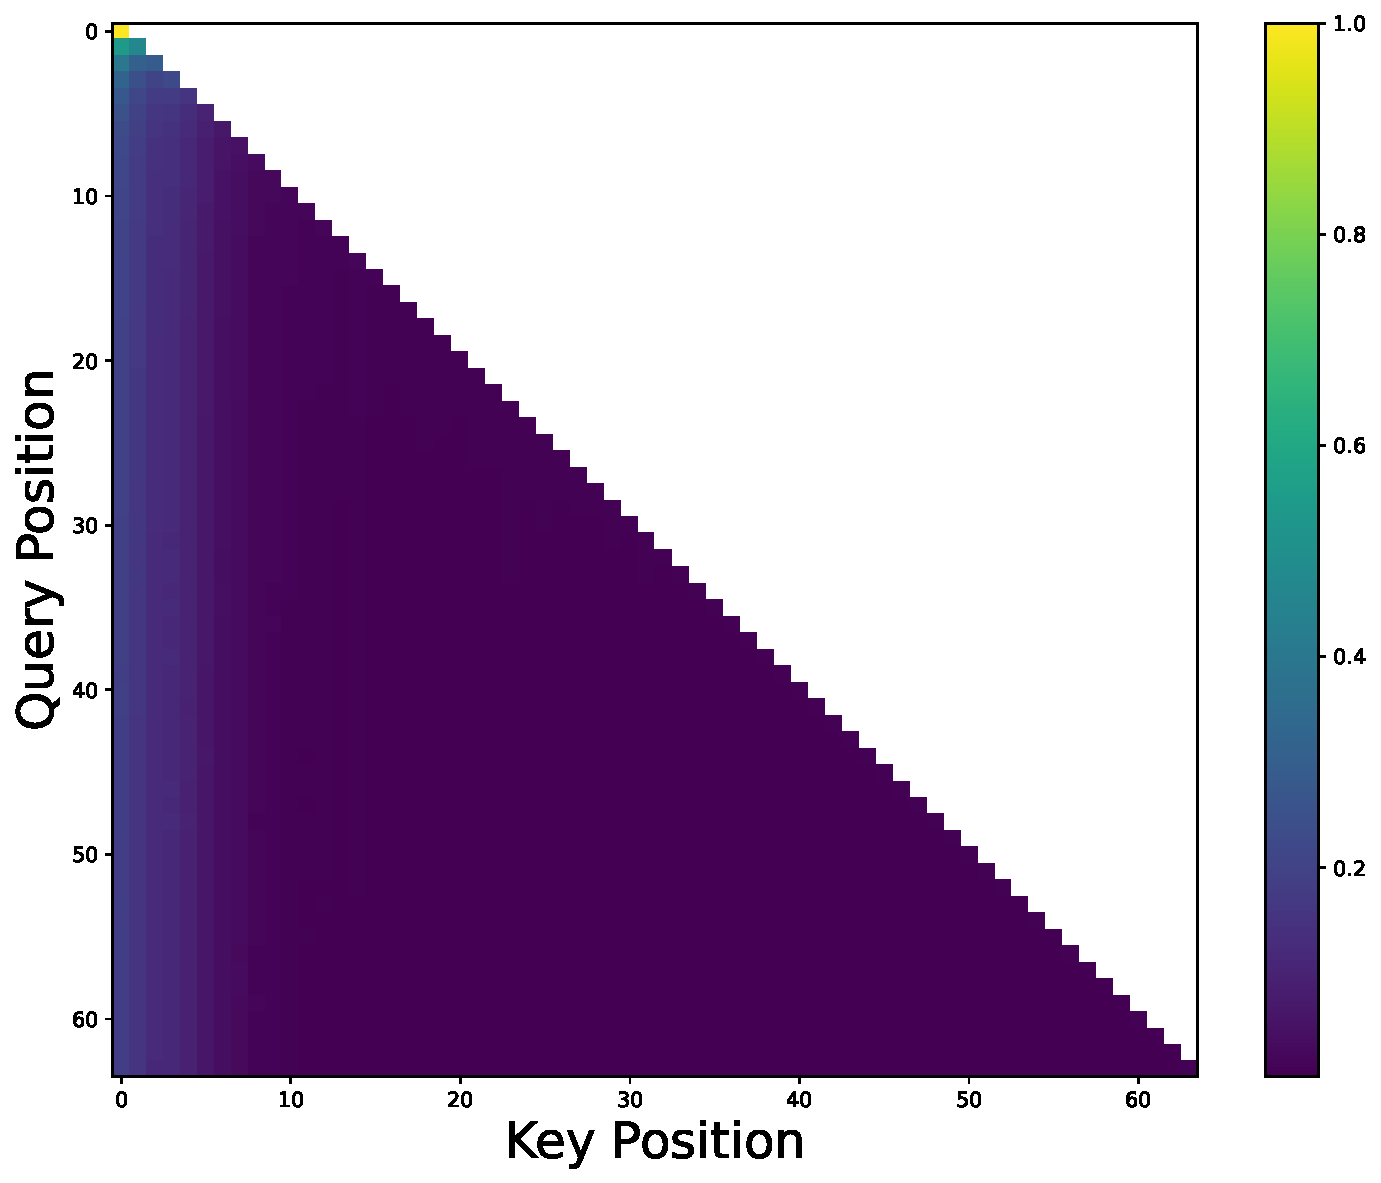
\includegraphics[width=\columnwidth]{figures/appendixA/layer36_attention.pdf}
    \end{subfigure}
    \begin{subfigure}[b]{0.33\linewidth} 
        \caption{\scriptsize{Layer 37}}
        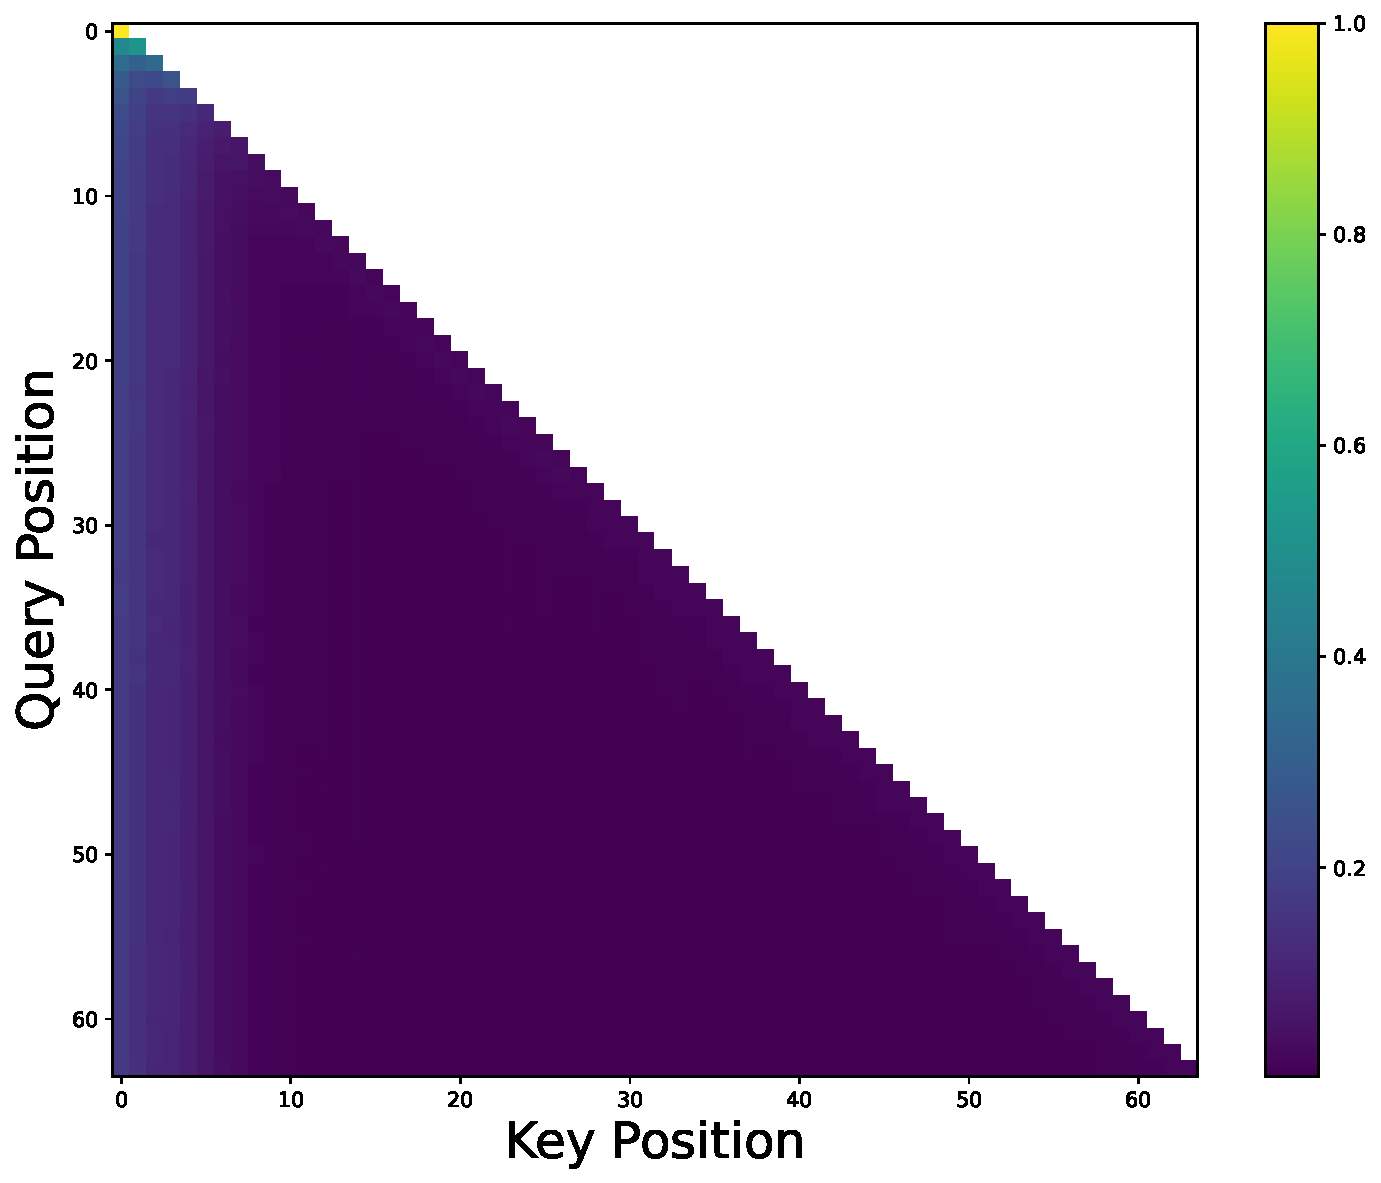
\includegraphics[width=\columnwidth]{figures/appendixA/layer37_attention.pdf}
    \end{subfigure}
    \begin{subfigure}[b]{0.33\linewidth} 
        \caption{\scriptsize{Layer 38}}
        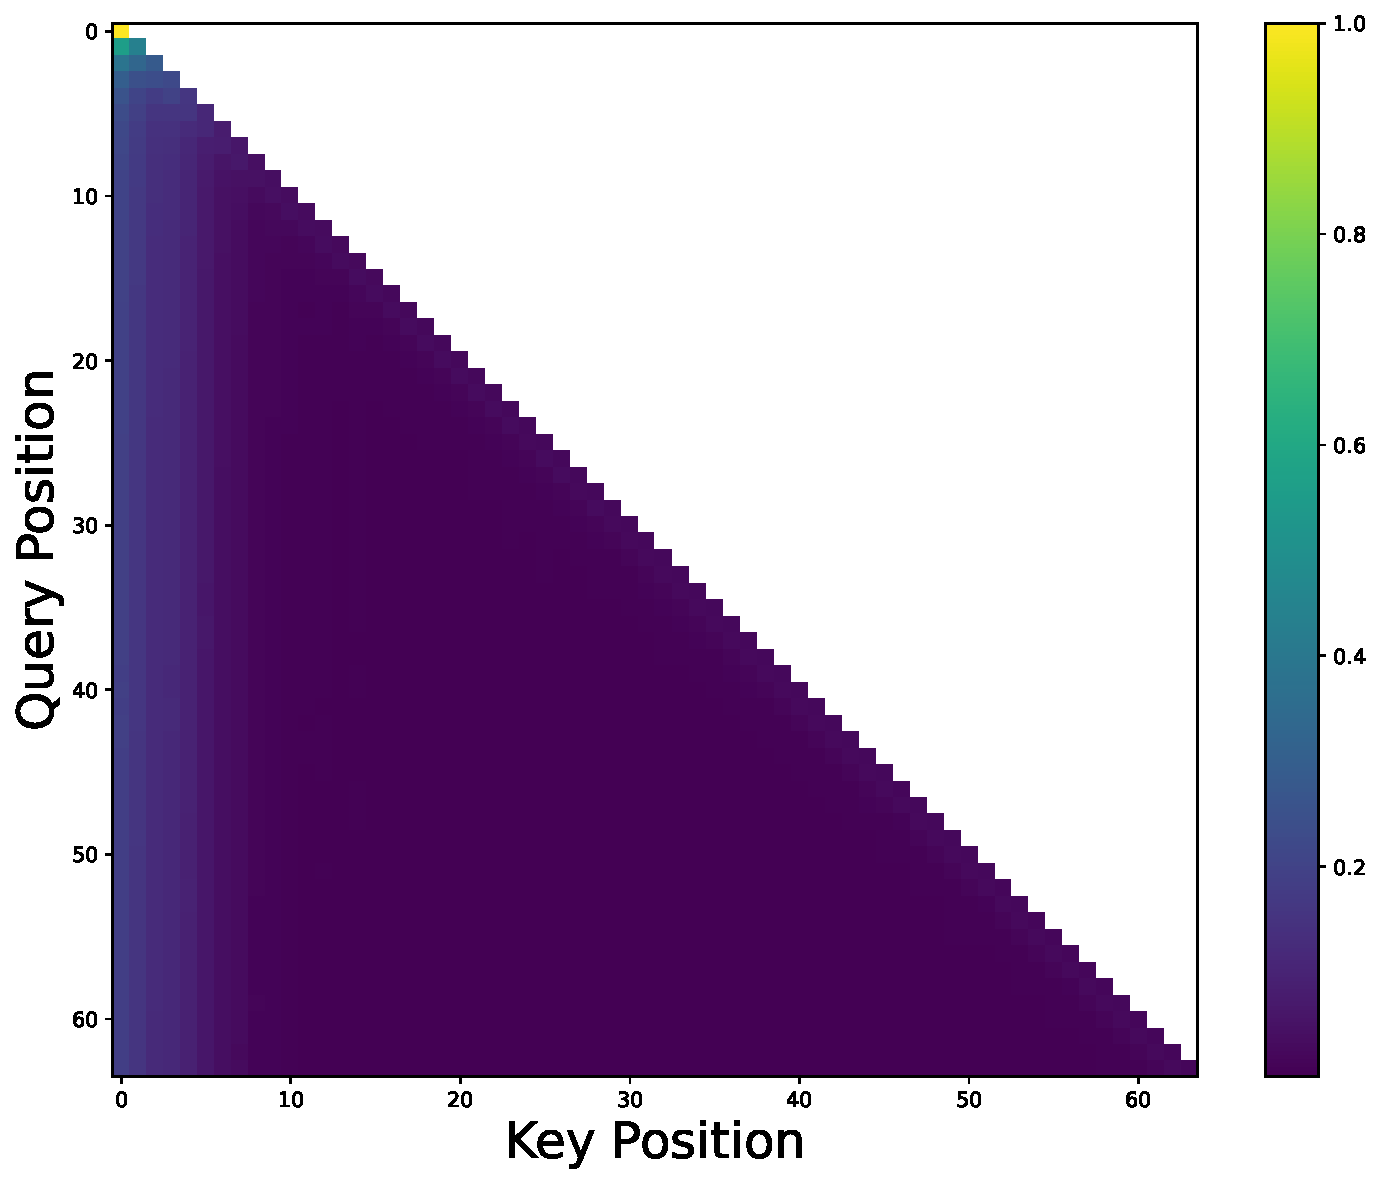
\includegraphics[width=\columnwidth]{figures/appendixA/layer38_attention.pdf}
    \end{subfigure}
    \begin{subfigure}[b]{0.33\linewidth} 
        \caption{\scriptsize{Layer 39}}
        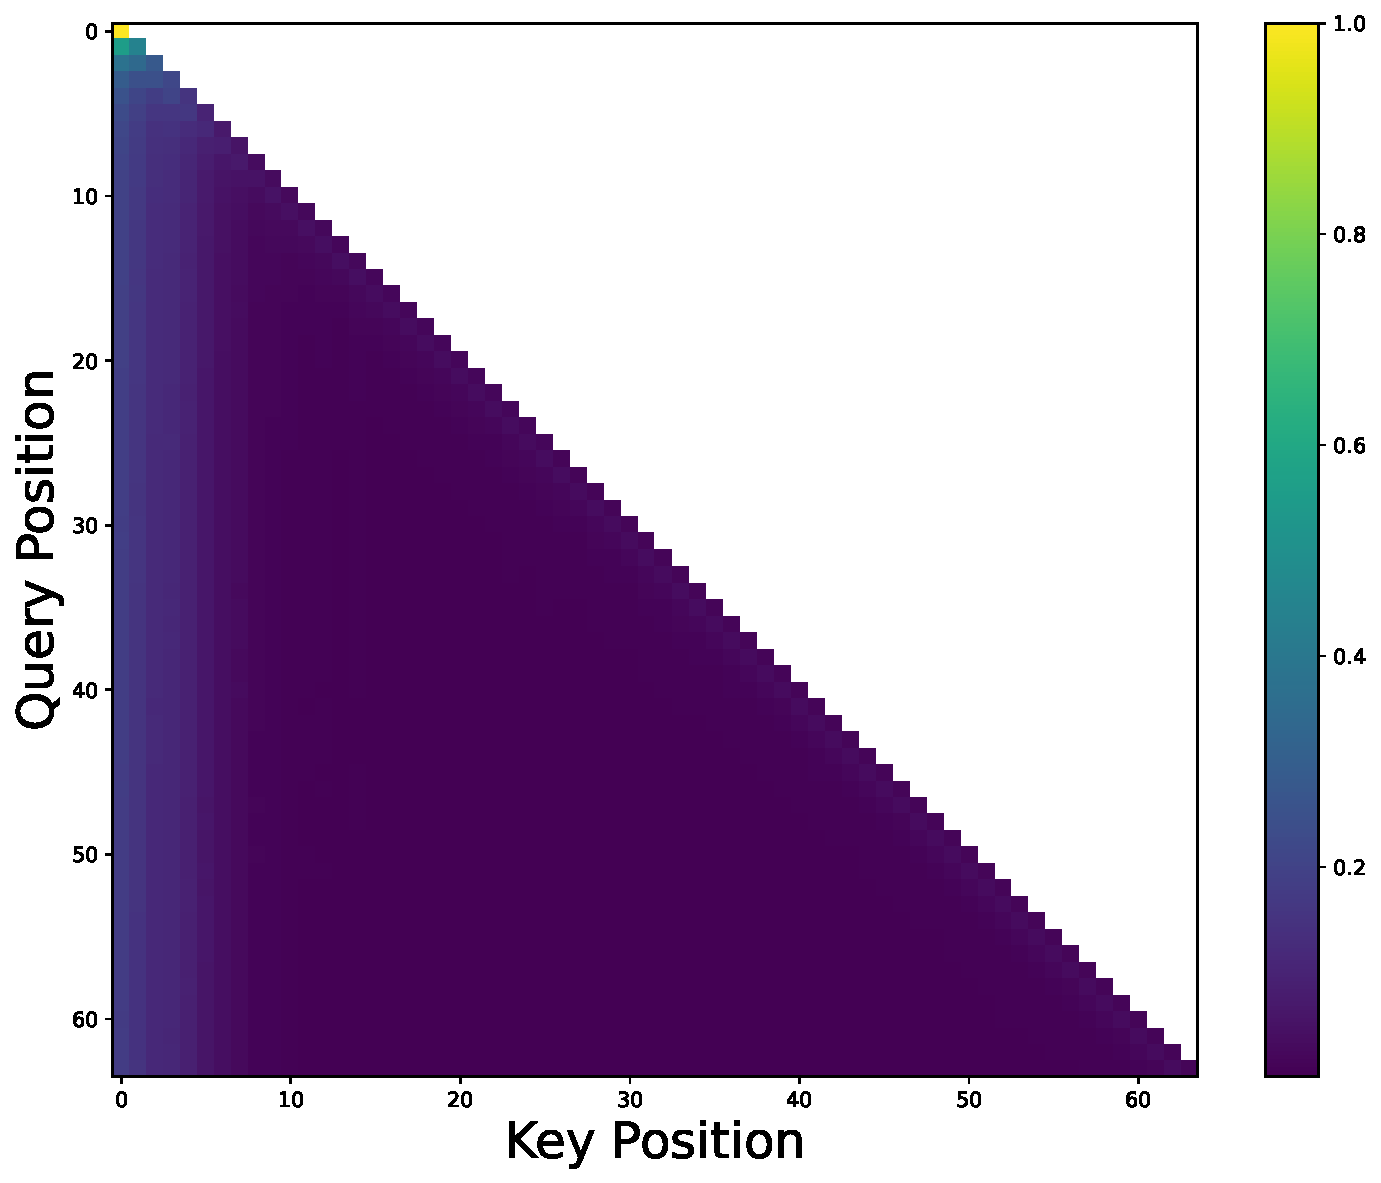
\includegraphics[width=\columnwidth]{figures/appendixA/layer39_attention.pdf}
    \end{subfigure}
    \caption{Mean attention maps from selected deep layers at step 30000. Notably, large $\ell_2$-norm hidden states at non-P0 positions do not noticeably affect the attention patterns, suggesting limited relevance to the sink mechanism. We leave further investigation to future work.}
\end{figure*}


\newpage

\section{Recent LLM's Statistics}
\label{appendix-recentllm}

\newcommand{\sinkLayerFigure}[4]{%
\begin{figure}[h]
    \centering
    % Left: Norm Plot
    \begin{subfigure}[c]{0.5\linewidth} 
        \centering
        \caption{\scriptsize{#1: $\ell_2$ Norm}}
        
\includegraphics[width=\linewidth]{figures/appendixB/combined_hidden_state_layerwise_no_bos/#2/combined_hidden_l2norm_layerwise.pdf}
    \end{subfigure}%
    \hspace{1.5em} 
    % Right: Heatmap
    \begin{subfigure}[c]{0.35\linewidth} 
        \centering
        \caption{\scriptsize{#1: Layer #3 Score}} 
        \includegraphics[width=\linewidth]{figures/appendixB/attention_heatmaps_per_layer_no_bos/#2/layer#3_attention.pdf}
    \end{subfigure}
    \caption{Layer-wise $\ell_2$ norm and attention sink visualization for #1. The attention sink becomes prominent after layer #3, coinciding with the sharp increase in the $\ell_2$ norm at position zero (P0).}
\end{figure}
}

\subsection{LLaMA-3 Series Analysis}

The LLaMA-3 family exhibits behaviors consistent with those discussed in the main text, and we omit further elaboration here for brevity.

\begin{figure*}[h]
    \centering
    \begin{minipage}[b]{0.4\linewidth} 
        \centering
        \begin{subfigure}[b]{0.95\linewidth} 
            \centering
            \caption{\scriptsize{Llama3.2-1B w/ \texttt{[BOS]}, $\ell_2$ Norm of Hidden States}}
            
\includegraphics[width=0.95\columnwidth]{figures/appendixB/combined_hidden_state_layerwise/Llama-3.2-1B-Instruct/combined_hidden_l2norm_layerwise.pdf}
        \end{subfigure}
        \begin{subfigure}[b]{0.47\linewidth} 
            \centering
            \caption{\scriptsize{Layer 1 Average Attention Score}}
            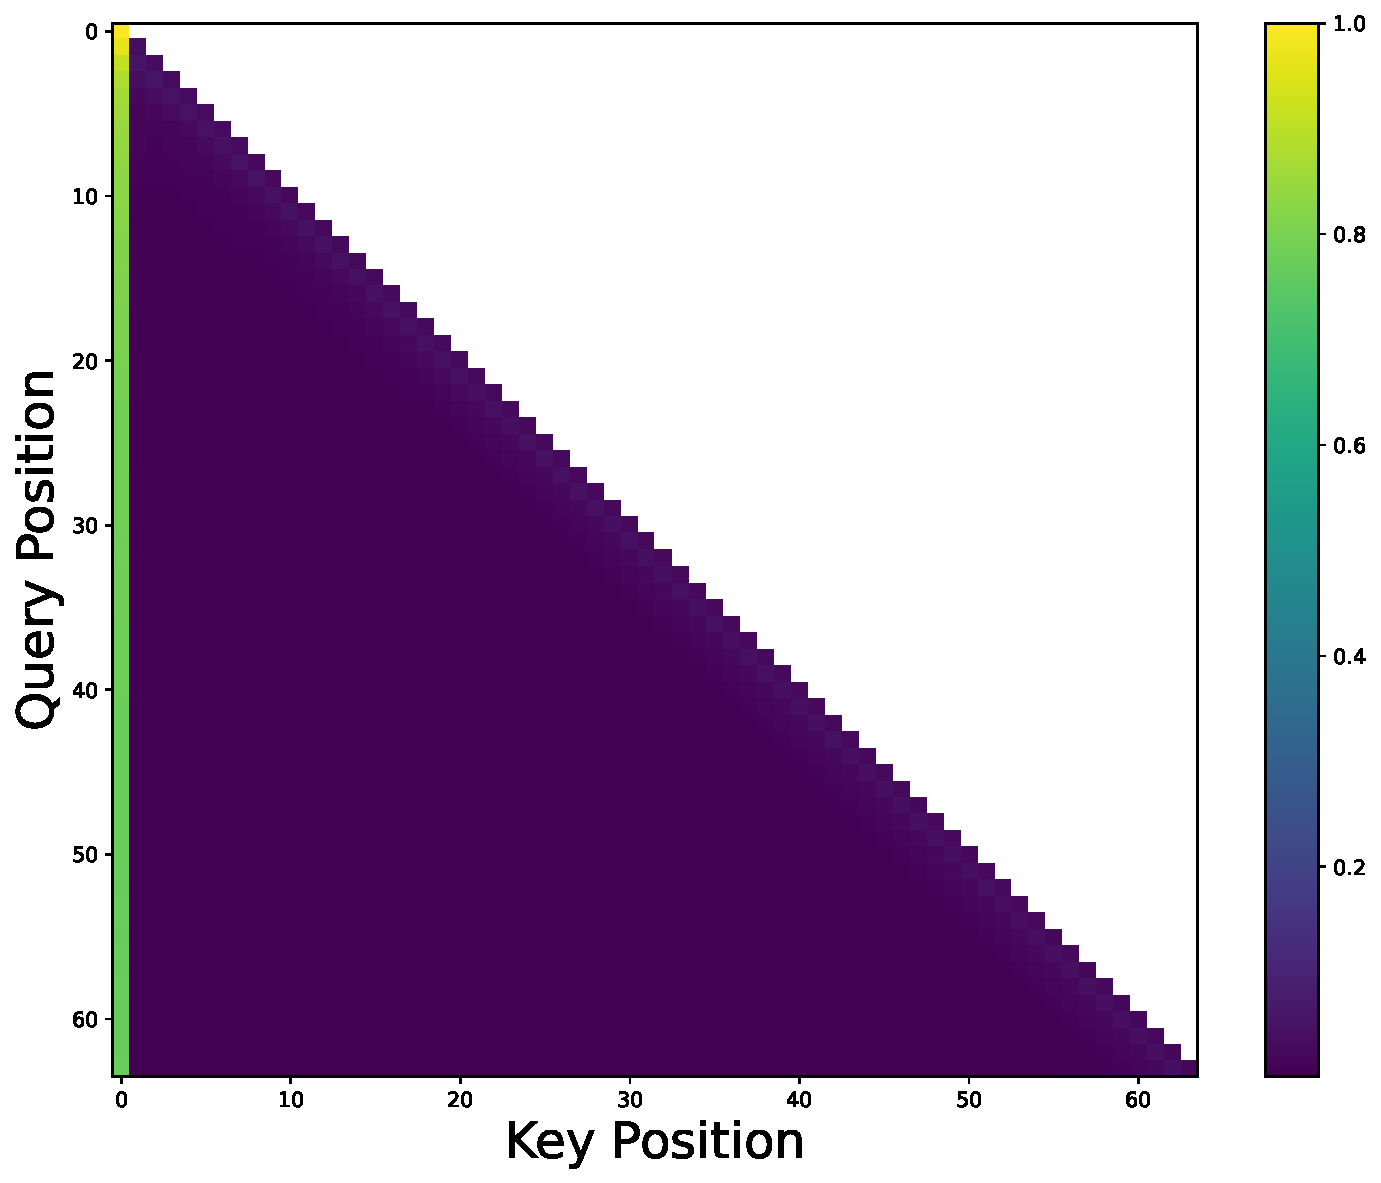
\includegraphics[width=\linewidth]{figures/appendixB/attention_heatmaps_per_layer/Llama-3.2-1B-Instruct/layer1_attention.pdf}
        \end{subfigure}
        \begin{subfigure}[b]{0.47\linewidth}
            \centering
            \caption{\scriptsize{Layer 2 Average Attention Score}} 
            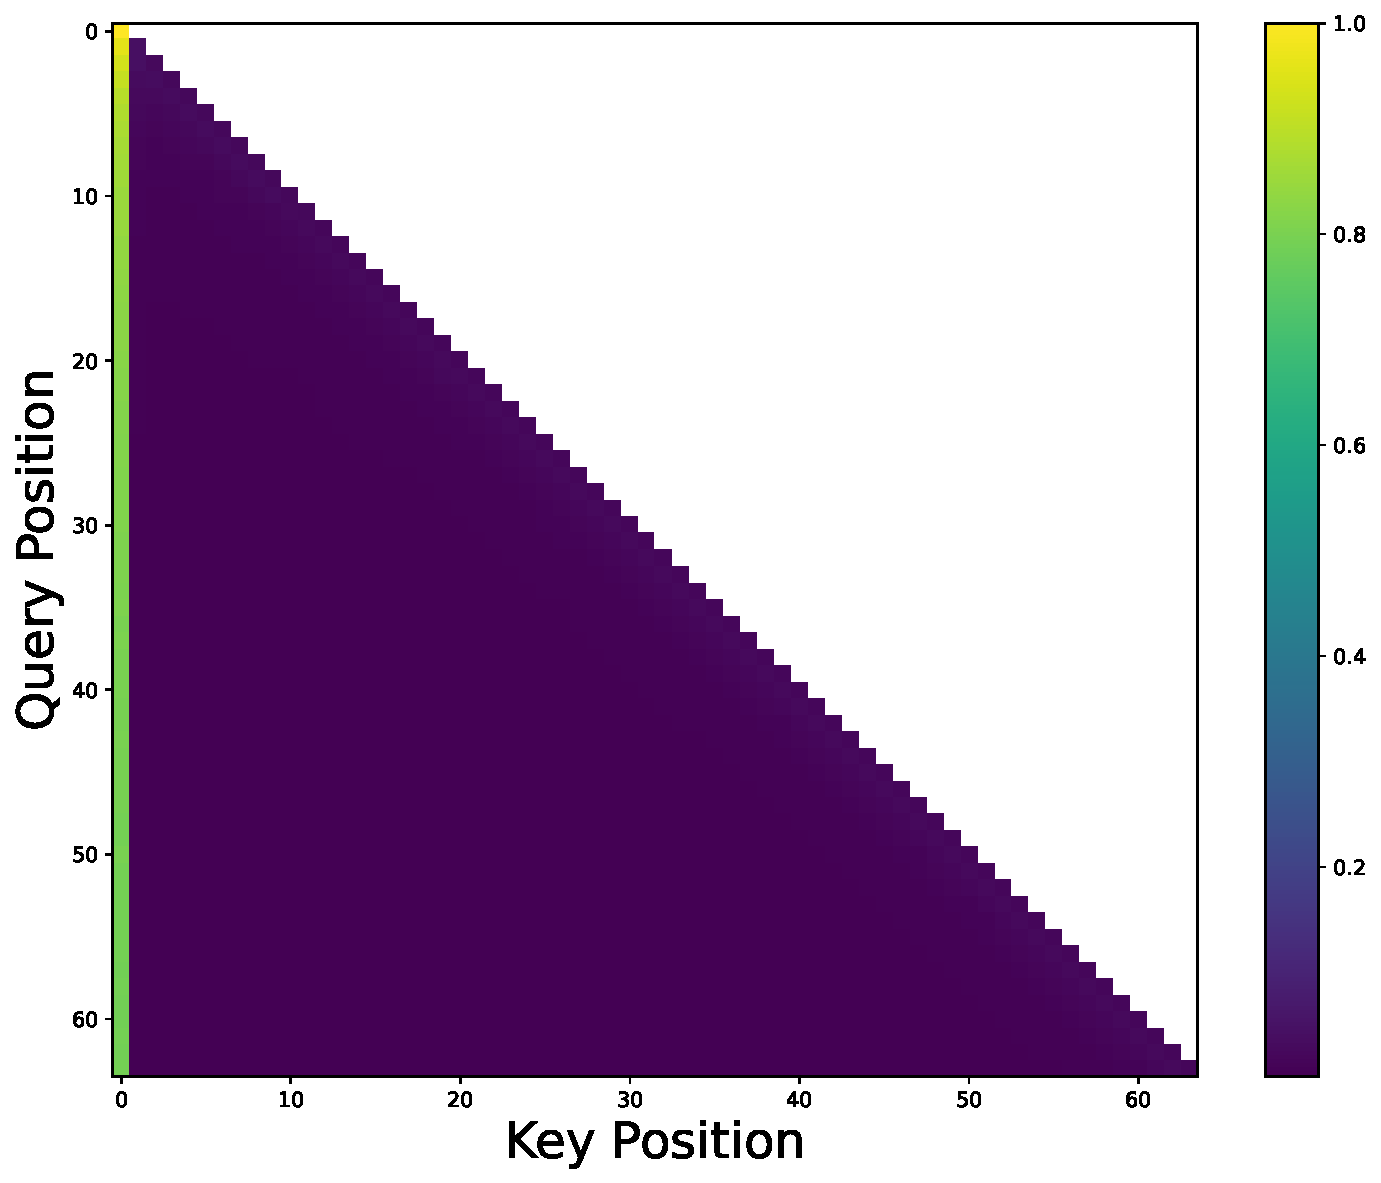
\includegraphics[width=\linewidth]{figures/appendixB/attention_heatmaps_per_layer/Llama-3.2-1B-Instruct/layer2_attention.pdf}
        \end{subfigure}
    \end{minipage}
    \begin{minipage}[b]{0.4\linewidth} 
        \centering
        \begin{subfigure}[b]{0.95\linewidth} 
            \centering
            \caption{\scriptsize{Llama3.2-1B w/o \texttt{[BOS]}, $\ell_2$ Norm of Hidden States}}
            
\includegraphics[width=0.95\columnwidth]{figures/appendixB/combined_hidden_state_layerwise_no_bos/Llama-3.2-1B-Instruct/combined_hidden_l2norm_layerwise.pdf}
        \end{subfigure}
        \begin{subfigure}[b]{0.47\linewidth} 
            \centering
            \caption{\scriptsize{Layer 1 Average Attention Score}}
            
\includegraphics[width=\linewidth]{figures/appendixB/attention_heatmaps_per_layer_no_bos/Llama-3.2-1B-Instruct/layer1_attention.pdf}
        \end{subfigure}
        \begin{subfigure}[b]{0.47\linewidth}
            \centering
            \caption{\scriptsize{Layer 2 Average Attention Score}} 
            
\includegraphics[width=\linewidth]{figures/appendixB/attention_heatmaps_per_layer_no_bos/Llama-3.2-1B-Instruct/layer2_attention.pdf}
        \end{subfigure}
    \end{minipage}
    \caption{Layer-wise $\ell_2$ norm of hidden states and attention score heat maps in LLaMA3.2-1B. Half-integer indices correspond to the output of attention modules after residual connection. Removing the \texttt{[BOS]} token eliminates the layer-1 attention sink and its associated $\ell_2$ norm amplification. However, due to renewed norm growth before layer 2, a position-zero (P0) sink re-emerges in the attention maps even in the absence of the \texttt{[BOS]} token.}
    \label{fig-llama1b}
    \vspace{-1em}
\end{figure*}

\begin{figure*}[h]
    \centering
    \begin{minipage}[b]{0.4\linewidth} 
        \centering
        \begin{subfigure}[b]{0.95\linewidth} 
            \centering
            \caption{\scriptsize{Llama3.2-3B w/ \texttt{[BOS]}, $\ell_2$ Norm of Hidden States}}
            
\includegraphics[width=0.95\columnwidth]{figures/appendixB/combined_hidden_state_layerwise/Llama-3.2-3B-Instruct/combined_hidden_l2norm_layerwise.pdf}
        \end{subfigure}
        \begin{subfigure}[b]{0.47\linewidth} 
            \centering
            \caption{\scriptsize{Layer 1 Average Attention Score}}
            
\includegraphics[width=\linewidth]{figures/appendixB/attention_heatmaps_per_layer/Llama-3.2-3B-Instruct/layer1_attention.pdf}
        \end{subfigure}
        \begin{subfigure}[b]{0.47\linewidth}
            \centering
            \caption{\scriptsize{Layer 2 Average Attention Score}} 
            
\includegraphics[width=\linewidth]{figures/appendixB/attention_heatmaps_per_layer/Llama-3.2-3B-Instruct/layer2_attention.pdf}
        \end{subfigure}
    \end{minipage}
    \begin{minipage}[b]{0.4\linewidth} 
        \centering
        \begin{subfigure}[b]{0.95\linewidth} 
            \centering
            \caption{\scriptsize{Llama3.2-3B w/o \texttt{[BOS]}, $\ell_2$ Norm of Hidden States}}
            
\includegraphics[width=0.95\columnwidth]{figures/appendixB/combined_hidden_state_layerwise_no_bos/Llama-3.2-3B-Instruct/combined_hidden_l2norm_layerwise.pdf}
        \end{subfigure}
        \begin{subfigure}[b]{0.47\linewidth} 
            \centering
            \caption{\scriptsize{Layer 1 Average Attention Score}}
            
\includegraphics[width=\linewidth]{figures/appendixB/attention_heatmaps_per_layer_no_bos/Llama-3.2-3B-Instruct/layer1_attention.pdf}
        \end{subfigure}
        \begin{subfigure}[b]{0.47\linewidth}
            \centering
            \caption{\scriptsize{Layer 2 Average Attention Score}} 
            
\includegraphics[width=\linewidth]{figures/appendixB/attention_heatmaps_per_layer_no_bos/Llama-3.2-3B-Instruct/layer2_attention.pdf}
        \end{subfigure}
    \end{minipage}
    \caption{Layer-wise $\ell_2$ norm of hidden states and attention score heat maps in LLaMA3.2-3B. Half-integer indices correspond to the output of attention modules after residual connection. Removing the \texttt{[BOS]} token eliminates the layer-1 attention sink and its associated $\ell_2$ norm amplification. However, due to renewed norm growth before layer 2, a position-zero (P0) sink re-emerges in the attention maps even in the absence of the \texttt{[BOS]} token.}
    \label{fig-llama3b}
    % \vspace{-2em}
\end{figure*}

\FloatBarrier
\newpage

\subsection{Mistral Analysis}

Mistral exhibits slightly different characteristics, which can be attributed to its two-phase training strategy. Initially trained with full attention on sequences matching the sliding window size, the model retains a position-zero attention sink. However, as it transitions to sliding window attention, its reliance on this early sink mechanism diminishes.

\begin{figure*}[h]
    \centering
    \begin{minipage}[b]{0.48\linewidth} 
        \centering
        \begin{subfigure}[b]{0.95\linewidth} 
            \centering
            \caption{\scriptsize{Mistral-v0.3-7B w/ \texttt{[BOS]}, $\ell_2$ Norm of Hidden States}}
            
\includegraphics[width=0.95\columnwidth]{figures/appendixB/combined_hidden_state_layerwise/Mistral-v0.3-7B-Instruct/combined_hidden_l2norm_layerwise.pdf}
        \end{subfigure}
        \begin{subfigure}[b]{0.47\linewidth} 
            \centering
            \caption{\scriptsize{Layer 1 Average Attention Score}}
            
\includegraphics[width=\linewidth]{figures/appendixB/attention_heatmaps_per_layer/Mistral-v0.3-7B-Instruct/layer1_attention.pdf}
        \end{subfigure}
        \begin{subfigure}[b]{0.47\linewidth}
            \centering
            \caption{\scriptsize{Layer 2 Average Attention Score}} 
            
\includegraphics[width=\linewidth]{figures/appendixB/attention_heatmaps_per_layer/Mistral-v0.3-7B-Instruct/layer2_attention.pdf}
        \end{subfigure}
    \end{minipage}
    \begin{minipage}[b]{0.48\linewidth} 
        \centering
        \begin{subfigure}[b]{0.95\linewidth} 
            \centering
            \caption{\scriptsize{Mistral-v0.3-7B w/o \texttt{[BOS]}, $\ell_2$ Norm of Hidden States}}
            
\includegraphics[width=0.95\columnwidth]{figures/appendixB/combined_hidden_state_layerwise_no_bos/Mistral-v0.3-7B-Instruct/combined_hidden_l2norm_layerwise.pdf}
        \end{subfigure}
        \begin{subfigure}[b]{0.47\linewidth} 
            \centering
            \caption{\scriptsize{Layer 1 Average Attention Score}}
            
\includegraphics[width=\linewidth]{figures/appendixB/attention_heatmaps_per_layer_no_bos/Mistral-v0.3-7B-Instruct/layer1_attention.pdf}
        \end{subfigure}
        \begin{subfigure}[b]{0.47\linewidth}
            \centering
            \caption{\scriptsize{Layer 2 Average Attention Score}} 
            
\includegraphics[width=\linewidth]{figures/appendixB/attention_heatmaps_per_layer_no_bos/Mistral-v0.3-7B-Instruct/layer2_attention.pdf}
        \end{subfigure}
    \end{minipage}
    \caption{Layer-wise $\ell_2$ norm of hidden states and attention score heat maps in . Half-integer indices correspond to the output of attention modules after residual connection. Removing the \texttt{[BOS]} token eliminates the layer-1 attention sink and its associated $\ell_2$ norm amplification. However, due to renewed norm growth before layer 2, a position-zero (P0) sink re-emerges in the attention maps even in the absence of the \texttt{[BOS]} token.}
    \label{fig-mistral}
    \vspace{-1em}
\end{figure*}

\newpage
\FloatBarrier

\newpage

\subsection{Pythia Series Analysis}

Smaller Pythia models such as Pythia-14M and Pythia-70M do not exhibit the emergence of a position-zero sink circuit. Notably, Pythia-160M fails to produce reliable statistics under float16 due to numerical instability. Interestingly, because all Pythia models are trained from scratch on the same number of tokens, we observe a non-monotonic trend as model size increases: larger models, despite having greater capacity, also face increased optimization difficulty, leading to a U-shaped pattern where the emergence layer of the sink first decreases and then increases. This suggests a trade-off between model expressivity and training convergence under fixed compute and data budgets.

\sinkLayerFigure{pythia-410m}{pythia-410m}{6}

\sinkLayerFigure{pythia-1b}{pythia-1b}{4}

\sinkLayerFigure{pythia-1.4b}{pythia-1.4b}{4}

\sinkLayerFigure{pythia-2.8b}{pythia-2.8b}{3}

\sinkLayerFigure{pythia-6.9b}{pythia-6.9b}{4}

\sinkLayerFigure{pythia-12b}{pythia-12b}{4}

\FloatBarrier

\subsection{Qwen2.5 Series Analysis}

By analyzing the Qwen2.5 series, we observe that models of different sizes are allocated varying training budgets. As a result, the final layer in which the sink-related circuit emerges shows no consistent pattern across model scales. Nevertheless, it is important to note that Qwen2.5 models were likely trained independently from scratch rather than derived from a single backbone. This helps explain why the 72B model achieves the best performance: it is not only the largest in size but also appears to be in the final stage of training and has likely received the most extensive token exposure.

\sinkLayerFigure{Qwen2.5-0.5B}{Qwen2.5-0.5B}{3}

\sinkLayerFigure{Qwen2.5-1.5B}{Qwen2.5-1.5B}{2}

\sinkLayerFigure{Qwen2.5-3B}{Qwen2.5-3B}{3}

\sinkLayerFigure{Qwen2.5-7B}{Qwen2.5-7B}{4}

\sinkLayerFigure{Qwen2.5-14B}{Qwen2.5-14B}{5}

\sinkLayerFigure{Qwen2.5-32B}{Qwen2.5-32B}{5}

\sinkLayerFigure{Qwen2.5-72B}{Qwen2.5-72B}{2}

\FloatBarrier

\newpage

\subsection{Qwen3 Series Analysis}

Our analysis of the Qwen series leads to several key observations. First, the Qwen3 models with 0.6B and 1.7B parameters exhibit highly similar behaviors, notably compressing the sink-related circuit into the first three layers. Second, although the 4B, 8B, 14B, and 32B variants of Qwen3 differ in depth, they all exhibit a strikingly consistent pattern: the attention sink becomes prominent at layer 7, coinciding with a sharp increase in the $\ell_2$ norm at position zero (P0). This consistency suggests that these models may not have been trained independently from scratch. Instead, it is likely that one of them served as a base model, with the others produced through scaling or pruning.

Moreover, in contrast to Qwen2, this behavior in Qwen3 suggests that it was trained on a smaller yet higher-quality dataset. Such data efficiency may explain why Qwen3 is able to achieve strong performance even before the sink circuit is fully compressed into the earliest layers. This observation provides additional insight into the design and training strategy of the Qwen3 family, pointing toward improved data curation and possible architectural reuse.

\textbf{Additionally, we observe that supervised fine-tuning (SFT) does not alter this pattern.}

\sinkLayerFigure{Qwen3-0.6B-Base}{Qwen3-0.6B-Base}{3}

\sinkLayerFigure{Qwen3-0.6B}{Qwen3-0.6B}{3}

\sinkLayerFigure{Qwen3-1.7B-Base}{Qwen3-1.7B-Base}{3}

\sinkLayerFigure{Qwen3-1.7B}{Qwen3-1.7B}{3}

\sinkLayerFigure{Qwen3-4B-Base}{Qwen3-4B-Base}{7}

\sinkLayerFigure{Qwen3-4B}{Qwen3-4B}{7}

\sinkLayerFigure{Qwen3-8B-Base}{Qwen3-8B-Base}{7}

\sinkLayerFigure{Qwen3-8B}{Qwen3-8B}{7}

\sinkLayerFigure{Qwen3-14B}{Qwen3-14B-Base}{7}

\sinkLayerFigure{Qwen3-14B}{Qwen3-32B}{7}

\sinkLayerFigure{Qwen3-30B-A3B-Base}{Qwen3-30B-A3B-Base}{2}

\sinkLayerFigure{Qwen3-30B-A3B}{Qwen3-30B-A3B}{2}



\FloatBarrier

\subsection{Olmo3 Series Analysis}

Olmo-3 adopts a hybrid architecture that combines full attention with a sliding window mechanism. Unlike Mistral, which requires a warm-up phase using full attention over shorter sequences to bootstrap learning, this hybrid design appears capable of training with sliding-window attention from scratch. A notable consequence is that, while Mistral still retains a persistent P0 sink, Olmo-3 exhibits no such pattern natively. Due to the lack of controlled comparisons between Olmo-3 and equivalent full-attention architectures, the downstream impact of this architectural choice remains unclear. We therefore report this observation without drawing further conclusions.

\sinkLayerFigure{Olmo-3-1025-7B}{Olmo-3-1025-7B}{10}

\sinkLayerFigure{Olmo-3-1125-32B}{Olmo-3-1125-32B}{10}

\newpage
\FloatBarrier

\subsection{OPT Serires Analysis}

Unlike many modern pretrained language models, the OPT series continues to adopt the original additive absolute positional encoding scheme—a method largely phased out due to its lack of extrapolation capability. This architectural choice allows the position embedding to directly influence the hidden states. As a result, the emergence of the P0 sink in OPT does not depend on an internal identification circuit, as observed in other models, but instead behaves more like models with explicit \texttt{[BOS]} tokens, where the sink effect is tightly coupled with the absolute position of the first token. Because removing the additive positional encoding would trigger severe out-of-distribution behavior, we do not conduct ablation experiments on OPT. Nonetheless, we include these models here for completeness.

\sinkLayerFigure{opt-125m}{opt-125m}{1}

\sinkLayerFigure{opt-350m}{opt-350m}{2}

\sinkLayerFigure{opt-1.3b}{opt-1.3b}{1}

\sinkLayerFigure{opt-2.7b}{opt-2.7b}{1}

\sinkLayerFigure{opt-6.7b}{opt-6.7b}{1}

\sinkLayerFigure{opt-13b}{opt-13b}{1}

\sinkLayerFigure{opt-30b}{opt-30b}{1}

\sinkLayerFigure{opt-66b}{opt-66b}{1}


\FloatBarrier

%%%%%%%%%%%%%%%%%%%%%%%%%%%%%%%%%%%%%%%%%%%%%%%%%%%%%%%%%%%%

% \newpage
% \input{sections/checklists}


\end{document}